Queremos observar que tan bueno es el algoritmo propuesto en la práctica. Para esto realizaremos una serie de tests utilizando las entradas que se utilizaron en el ejericio 3. Además, agregaremos los casos de entrada con solución óptima, ya que en principio, se desconoce la calidad del resultado y el algoritmo no tiene un tiempo de parada prefijado, con lo que estos casos pueden aportar conocimientos nuevos sobre el comportamiento de tabú search.\\
La idea es tratar de encontrar la configuración ideal para que en promedio el algoritmo resuelva la mayoria de los casos eficientemente. Para lograr esto, debemos experimentar variando distintos parametros para cada entrada y obtener las respectivas conclusiones de los resultados obtenidos.\\
Los parámetros de estudio serán:

\begin{enumerate}
\item  \textbf{Cantidad de iteraciones}: Tenemos que observar en promedio, cuantas iteraciones conviene tomar para obtener un buen resutado.
\item \textbf{Tenor tabú}: Tenemos que observar que sucede al aumentar el tenor tabú, y hasta cuanto es conveniente hacerlo para obtener un buen resultado.
\item \textbf{Atributos tabú}: Analizar que sucede al tomar como atributos tabú las aristas que cambiaron o las aristas nuevas
\item \textbf{Función de aspiración}: Elegir la solución más tabú o la menos tabú.
\end{enumerate}

Se tomarán 30 mediciones por cada tipo de test. En el caso de 1) y 2), por cada aumento realizado. Se tomará una media alfa podada de las mismas con $\alpha$ = 0.5 de manera de podar un 25\% de los datos a cada lado. De esta forma se reducen los outliers en las muestras consideradas. 
Además se tomará la varianza muestral usando la media calculada y las mediciones que queden luego de aplicar la media.\\

Como fue enunciado en incisos anteriores de este trabajo las 4 familias en las que la heur\'istica golosa no otorga una soluci\'on \'optima son:

\begin{enumerate}
\item Familia 4
\item Familia 6
\item Familia 7
\item Familia 8
\end{enumerate}

Estas ser\'an las unicas a ser a analizadas, ya que el resto no presentan una mejora para ser alcanzada o no tienen soluci\'on
 

\subsubsection*{Familia 4}

\vspace*{0.3cm} \vspace*{0.3cm}
  \begin{center}
 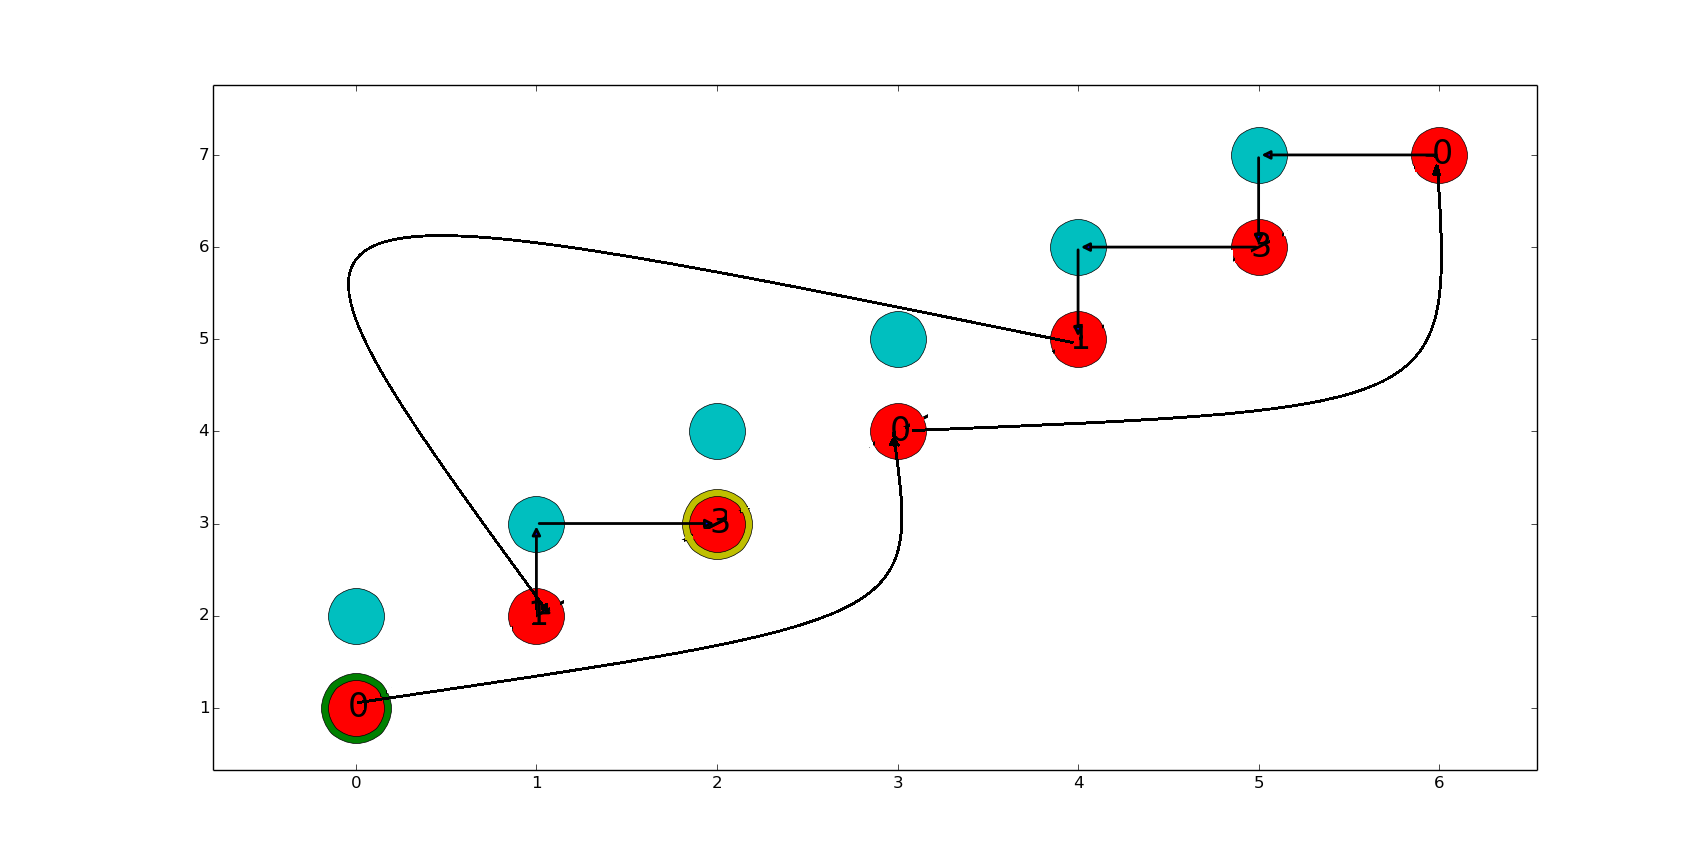
\includegraphics[scale=0.3]{./EJ4/fam4goloso.png}\\
 {            \textit{Soluci\'on Golosa}}
  \end{center}
  \vspace*{0.3cm}

\vspace*{0.3cm} \vspace*{0.3cm}
  \begin{center}
 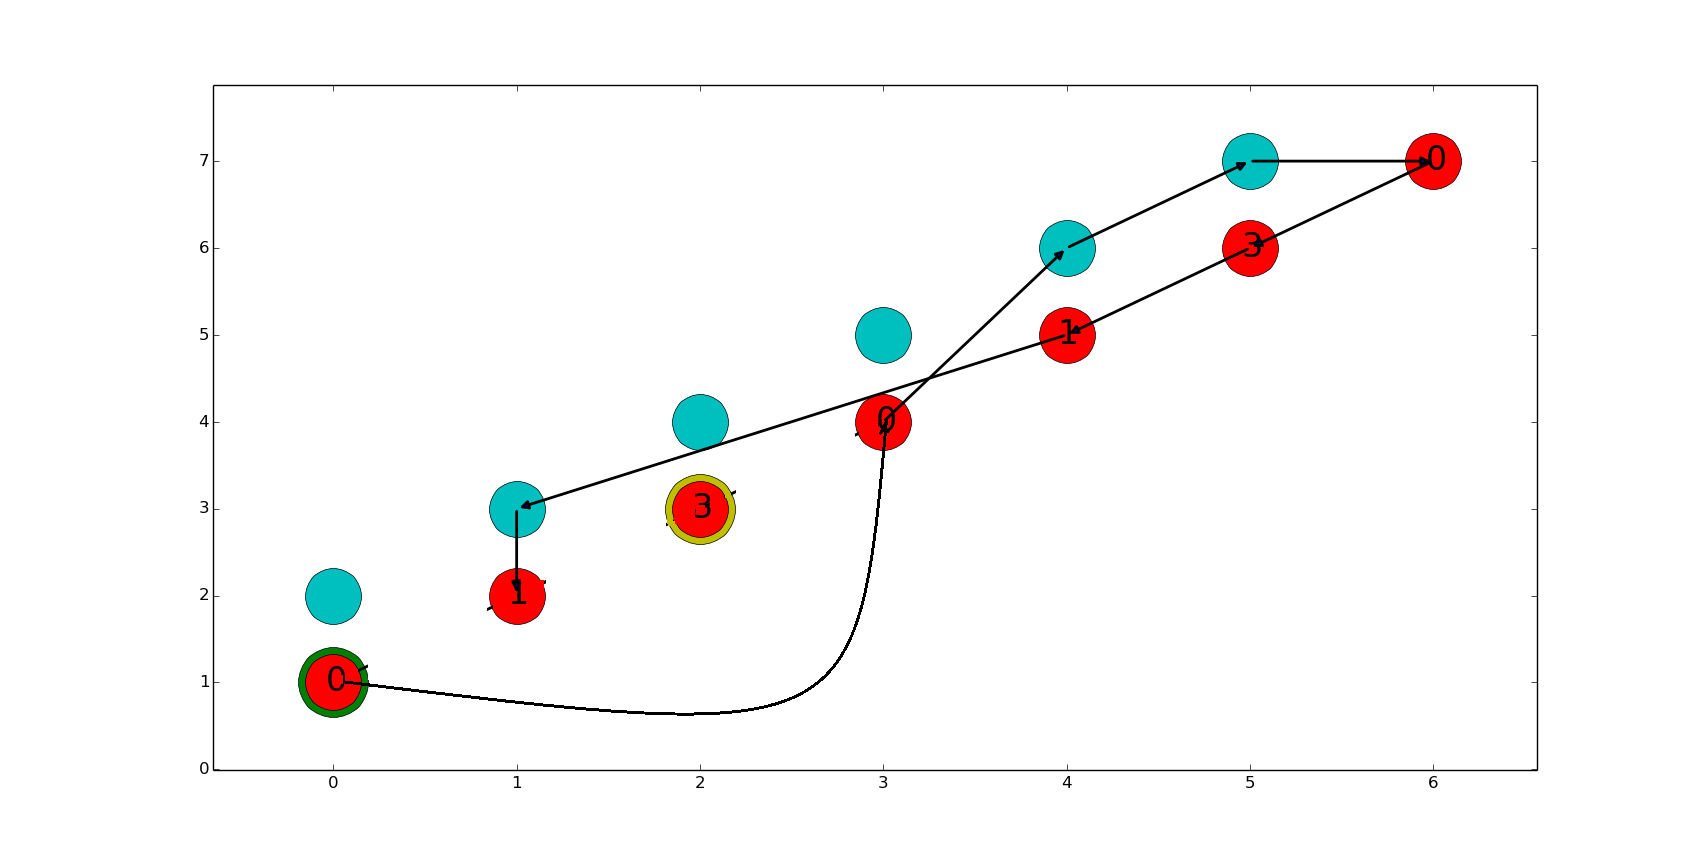
\includegraphics[scale=0.3]{./EJ4/fam42opt.png}\\
 {            \textit{Soluci\'on 2-OPT}}
  \end{center}
  \vspace*{0.3cm}

\vspace*{0.3cm} \vspace*{0.3cm}
  \begin{center}
 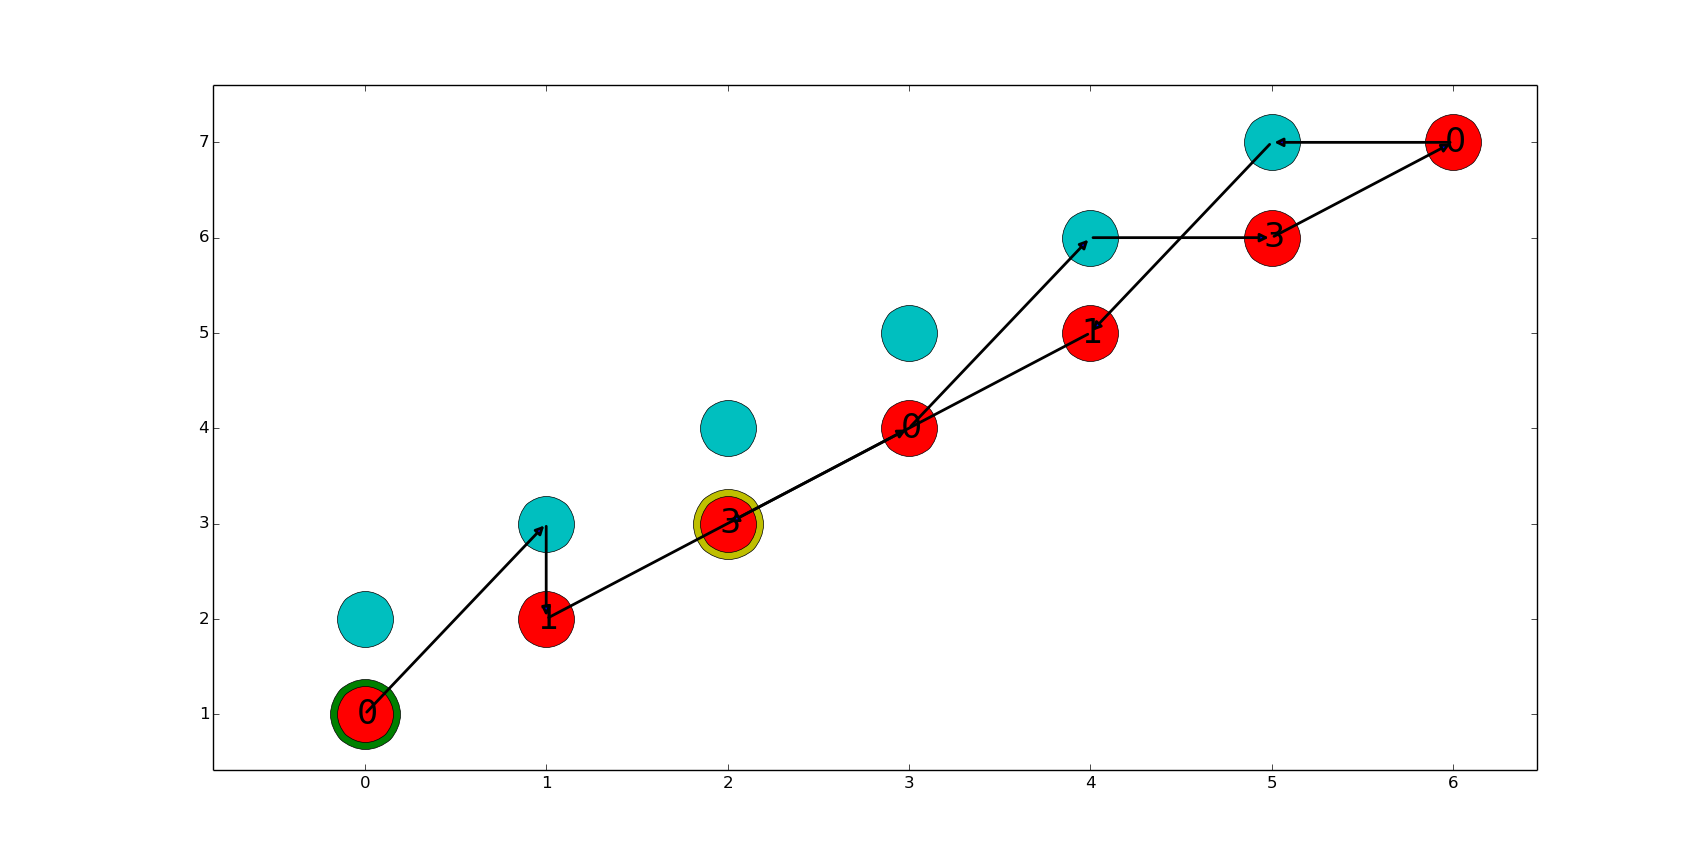
\includegraphics[scale=0.3]{./EJ4/fam43opt.png}\\
 {            \textit{Soluci\'on 3-OPT}}
  \end{center}
  \vspace*{0.3cm}

-----> ACOMODARLO

Nos parecio prudente corroborar cada heuristica del tabu search con la correspondiente busqueda local, para corroborar si la misma mejora o empeora y luego corroborar cual de las elegidas para dicho tabu es la mejor en relaci\'on tiempo-calidad de soluci\'on.

Veamos como se comporta Tabu 2-OPT con respecto a la heuristica de busqueda local 2-OPT:

\vspace*{0.3cm} \vspace*{0.3cm}
  \begin{center}
 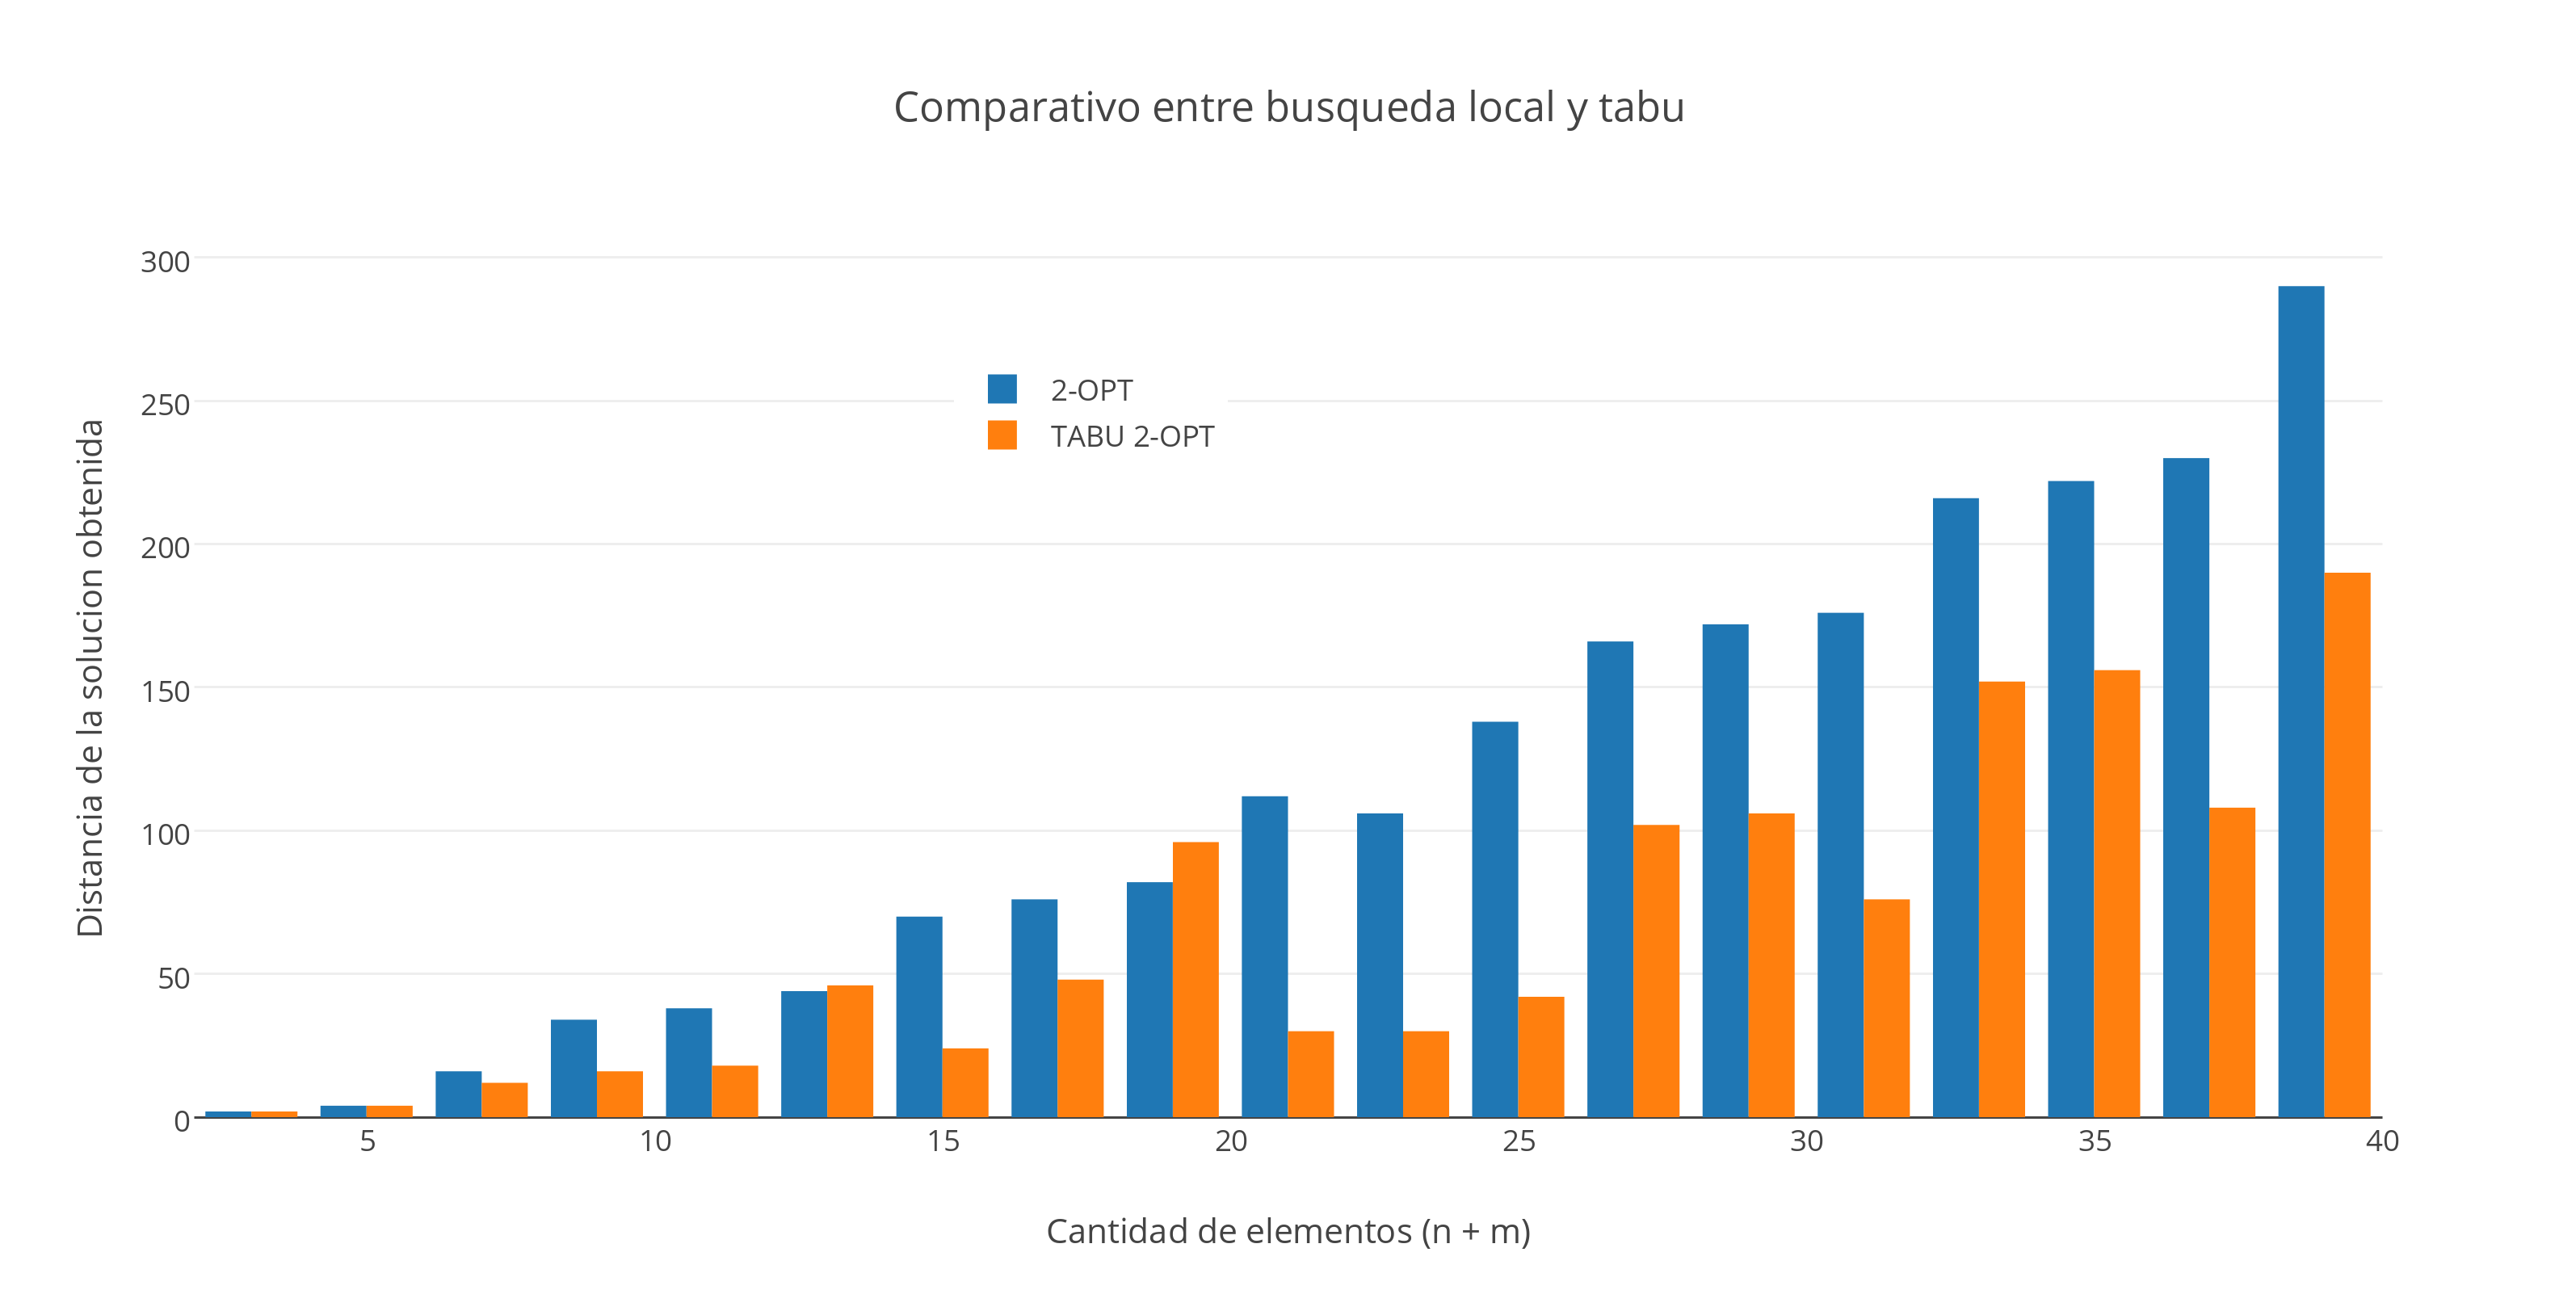
\includegraphics[scale=0.5]{./EJ4/comparativogym02opt.png}\\
 {            \textit{Gráfico \ 4.1 - 2-OPT vs Tabu 2-OPT sobre Familia 4}}
  \end{center}
  \vspace*{0.3cm}

En cuanto a tiempo insumido vemos lo siguiente:

\vspace*{0.3cm} \vspace*{0.3cm}
  \begin{center}
 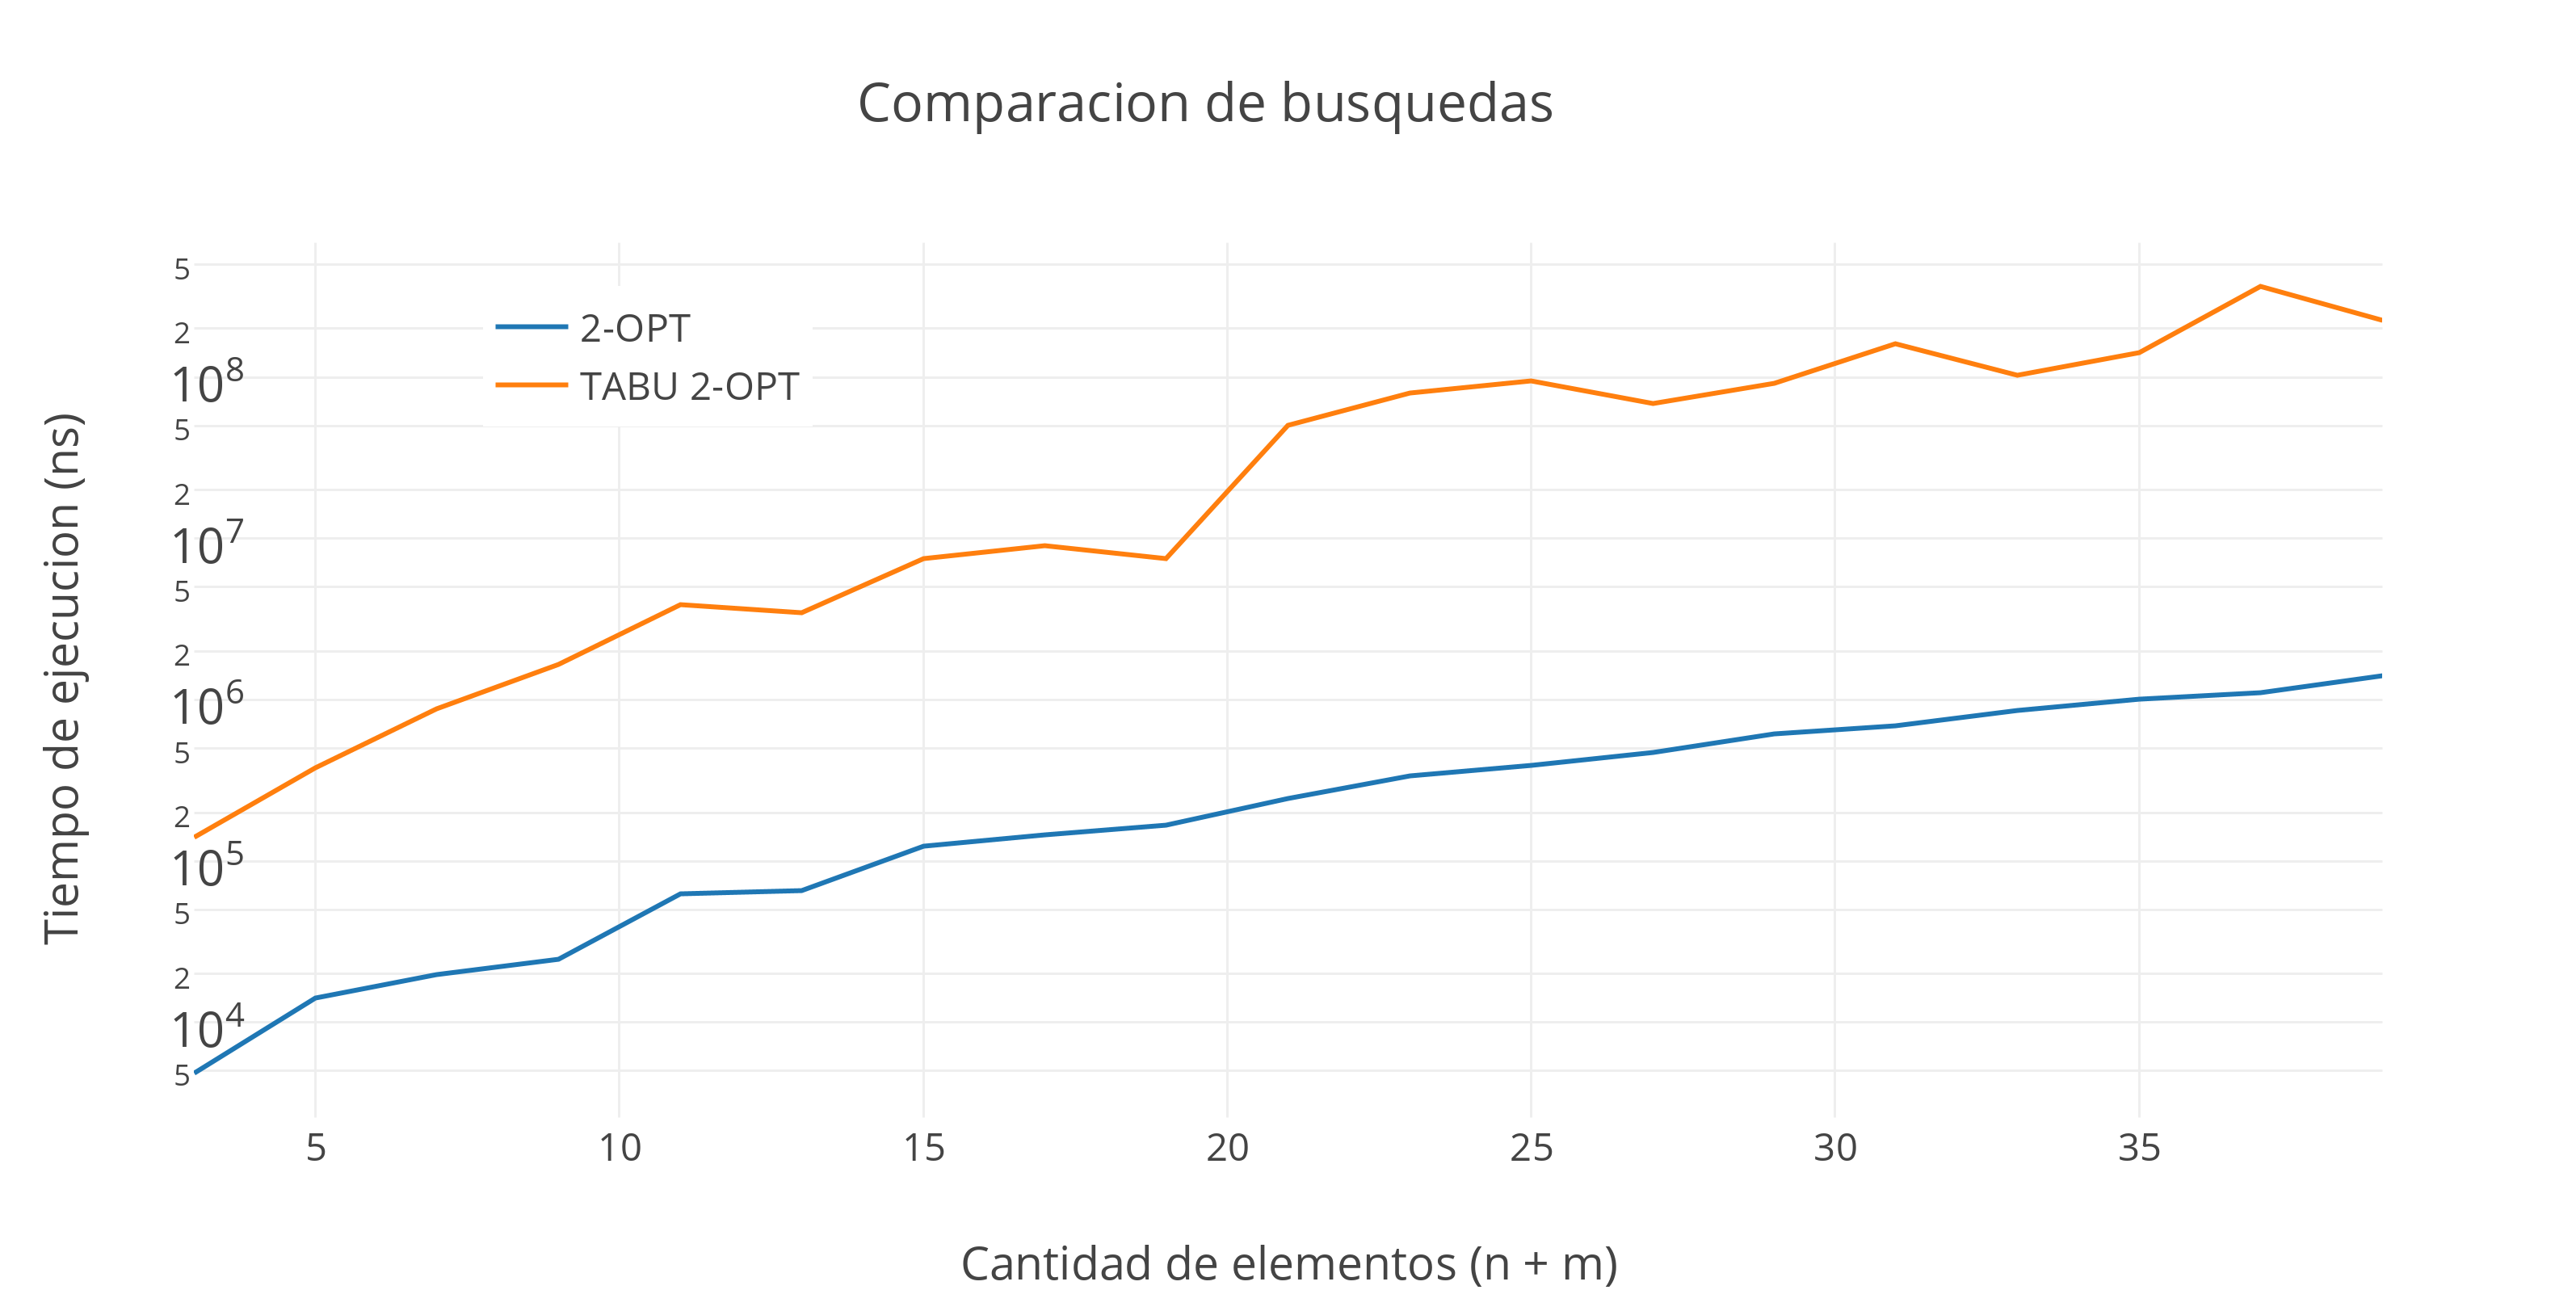
\includegraphics[scale=0.5]{./EJ4/medicion2optgym0.png}\\
 {            \textit{Gráfico \ 4.2 - 2-OPT vs Tabu 2-OPT sobre Familia 4}}
  \end{center}
  \vspace*{0.3cm}


Luego, para 3-OPT:

\vspace*{0.3cm} \vspace*{0.3cm}
  \begin{center}
 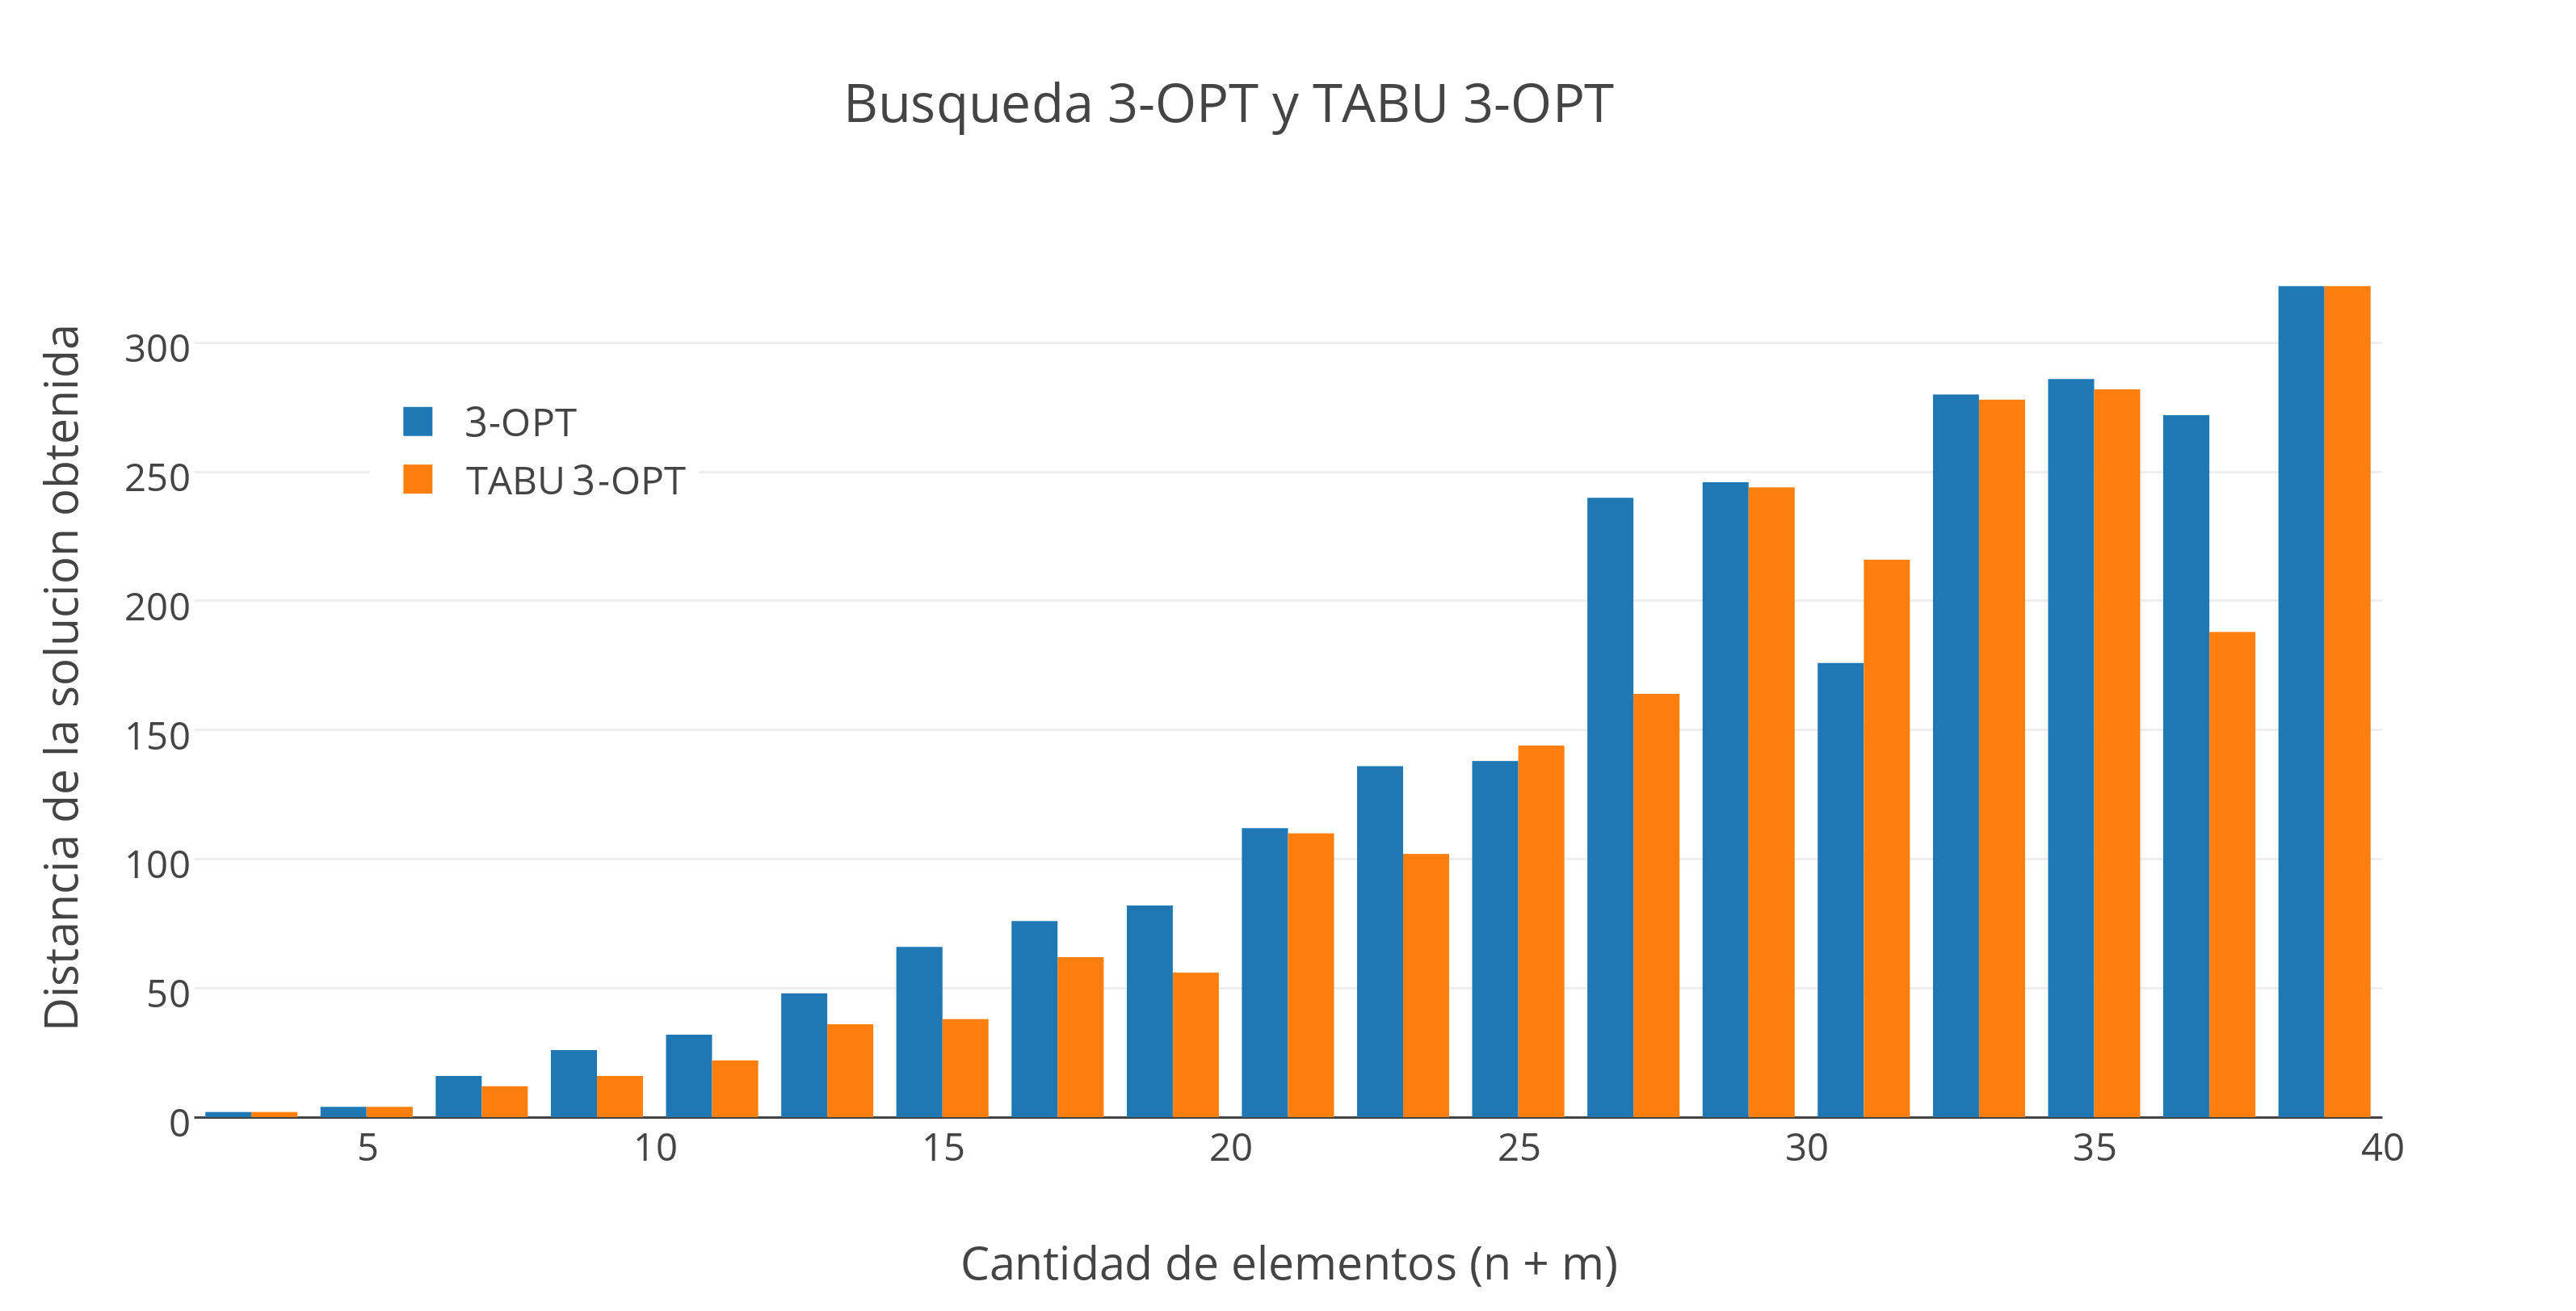
\includegraphics[scale=0.5]{./EJ4/comparativogym03opt.png}\\
 {            \textit{Gráfico \ 4.3 - 3-OPT vs Tabu 3-OPT sobre Familia 4}}
  \end{center}
  \vspace*{0.3cm}

En cuanto a tiempo insumido vemos lo siguiente:

\vspace*{0.3cm} \vspace*{0.3cm}
  \begin{center}
 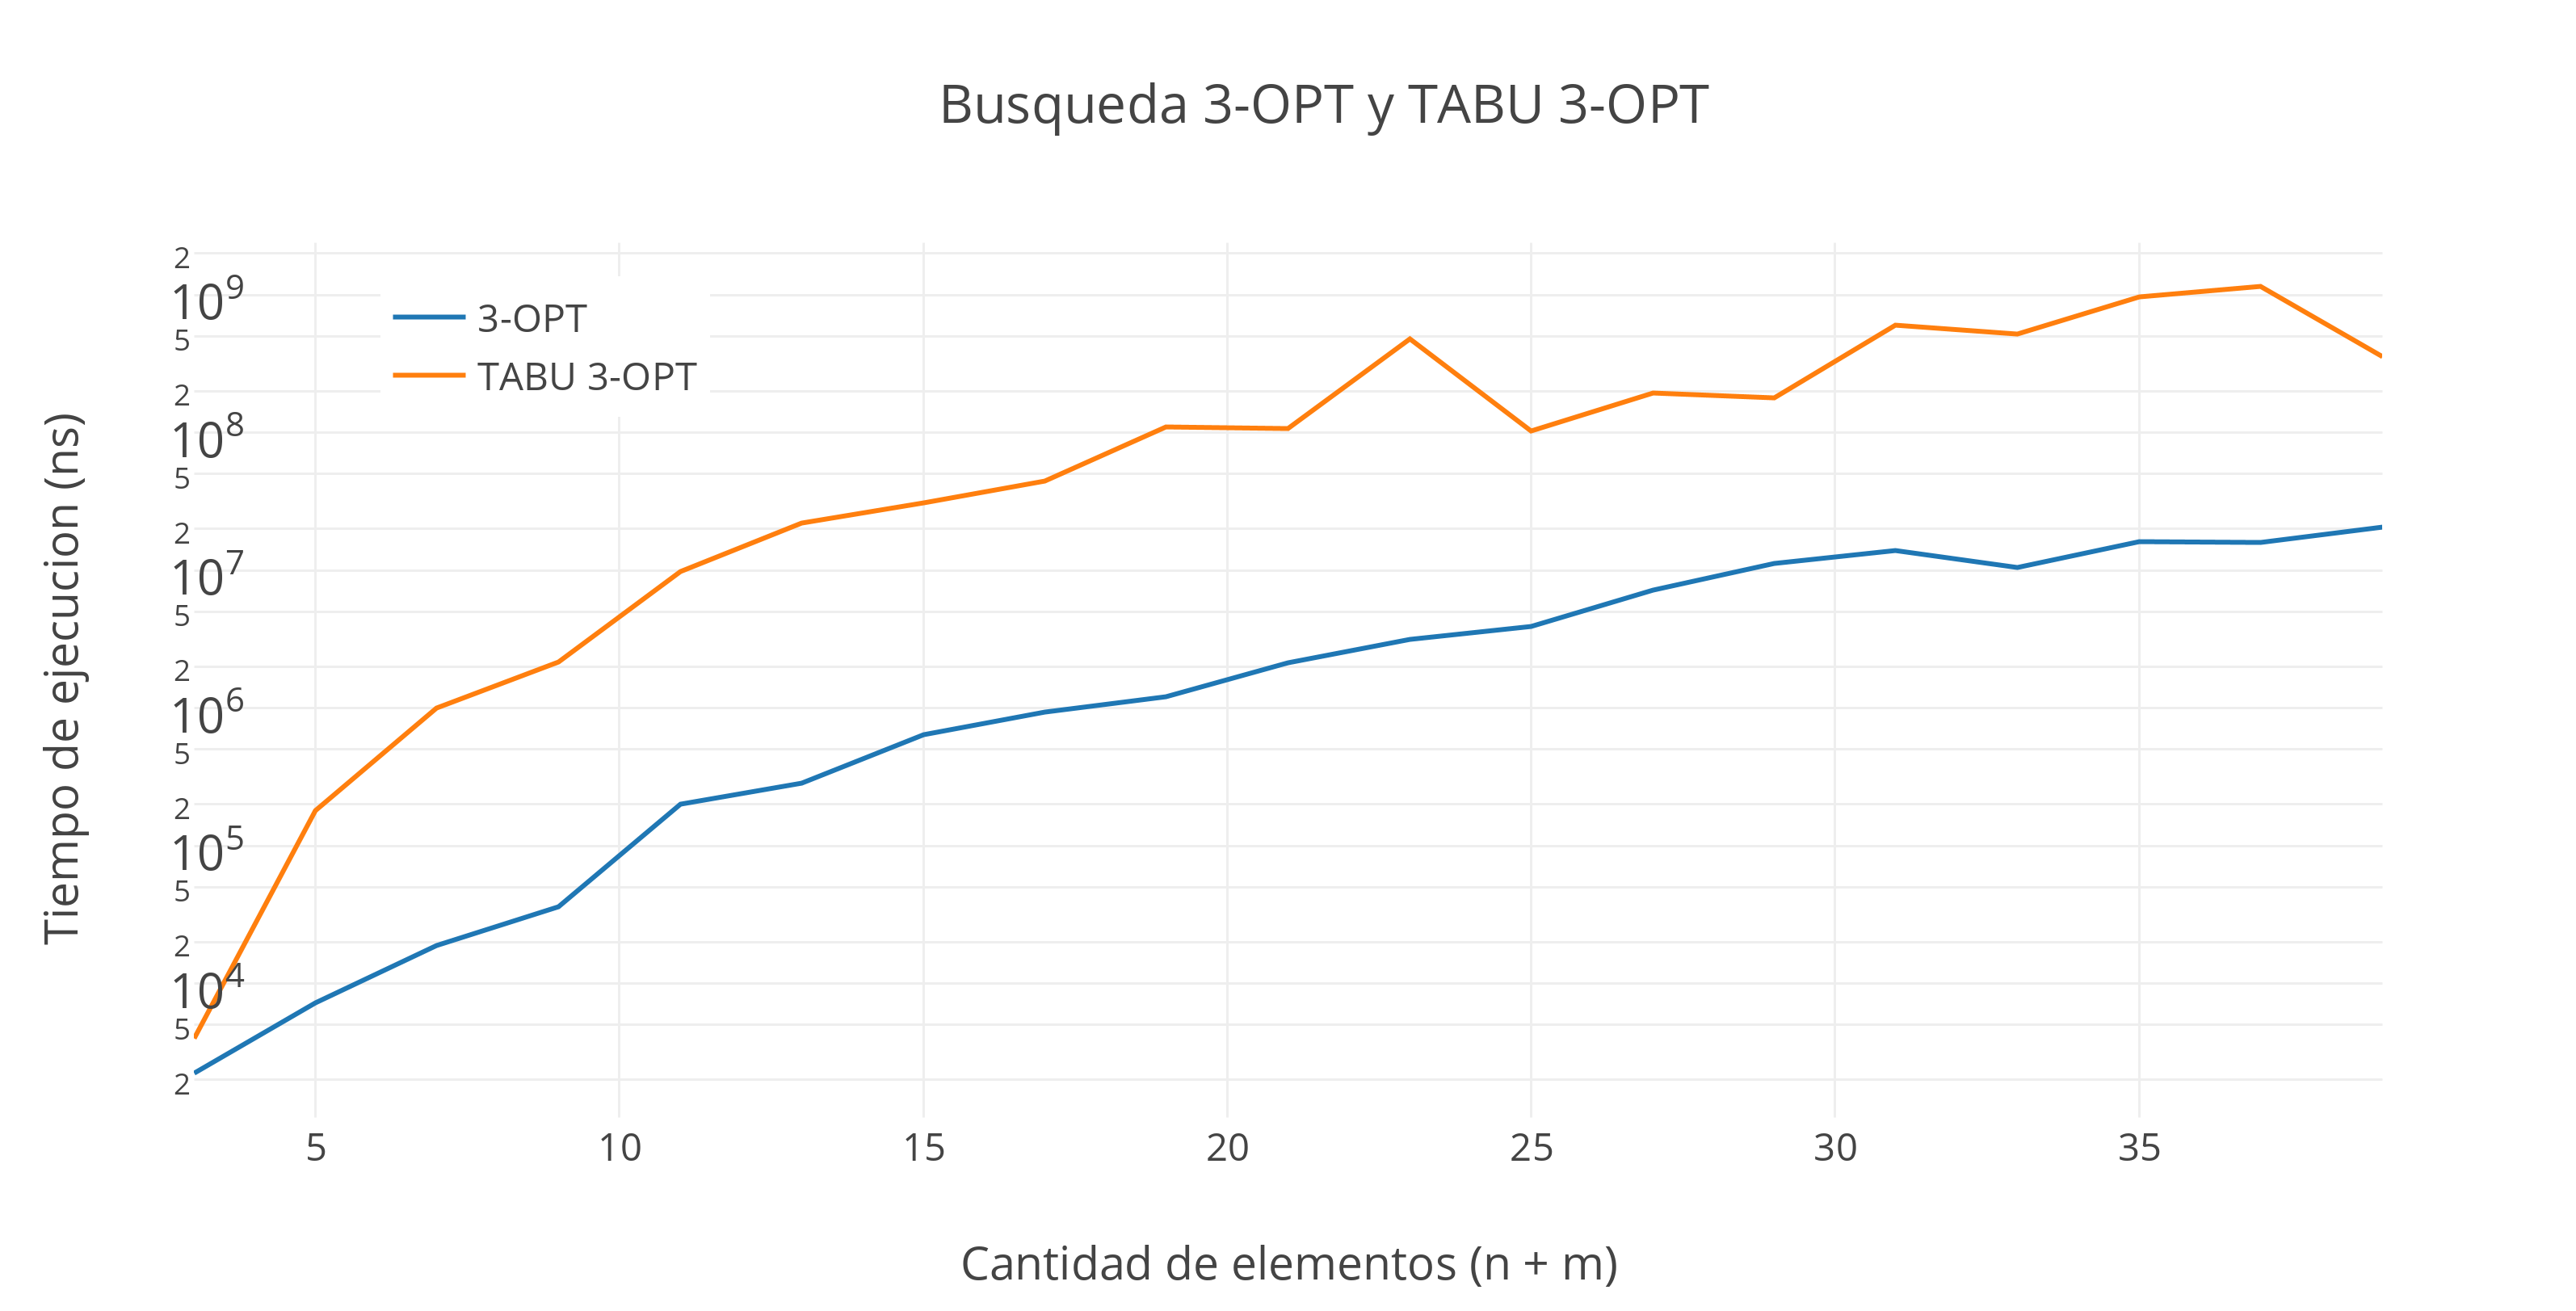
\includegraphics[scale=0.5]{./EJ4/medicion3optgym0.png}\\
 {            \textit{Gráfico \ 4.4 - 3-OPT vs Tabu 3-OPT sobre Familia 4}}
  \end{center}
  \vspace*{0.3cm}
  
Para la comparación entre algoritmos tabu, se comparará conjuntamente el tiempo de ejecución con la calidad de la solución. Para esta última tendremos en cuenta que los algoritmos, de devolver un resultado, será válido: esto quiere decir que cuanto menor distancia recorran en las soluciones, mejor serán las mismas:

Las soluciones obtenidas fueron las siguientes:

\vspace*{0.3cm} \vspace*{0.3cm}
  \begin{center}
 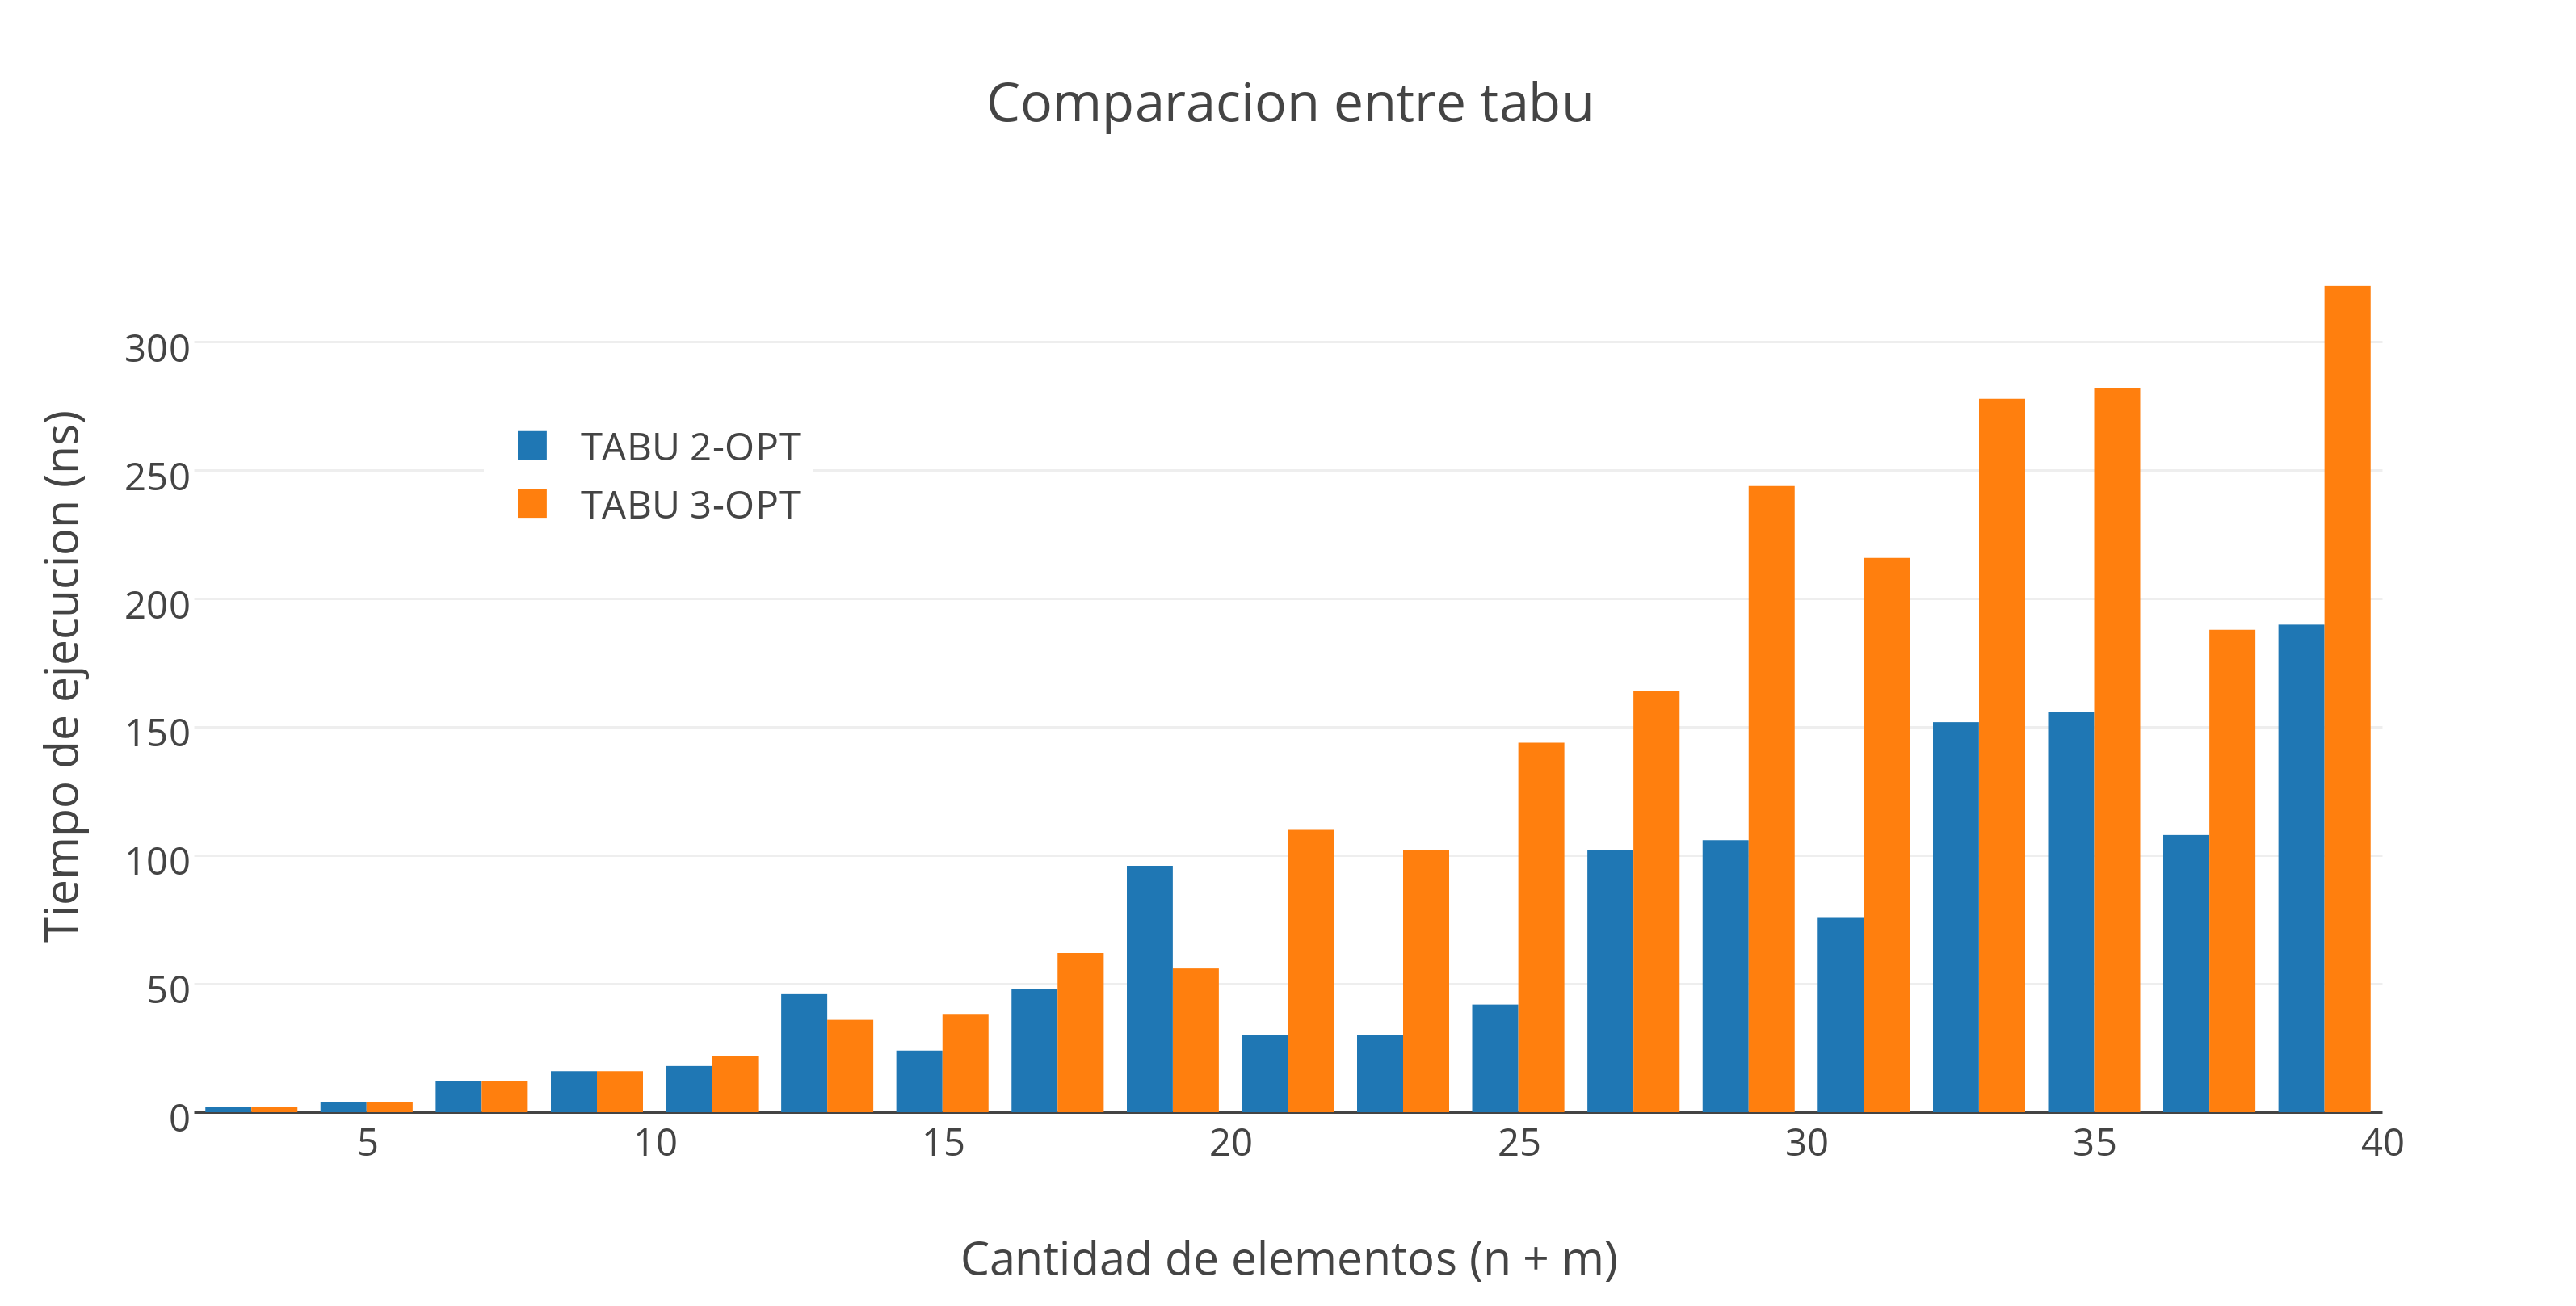
\includegraphics[scale=0.5]{./EJ4/comparativogym0.png}\\
 {            \textit{Gráfico \ 4.5 - Tabu 2-OPT vs Tabu 3-OPT sobre Familia 4}}
  \end{center}
  \vspace*{0.3cm}

En cuanto a tiempo insumido vemos lo siguiente:

\vspace*{0.3cm} \vspace*{0.3cm}
  \begin{center}
 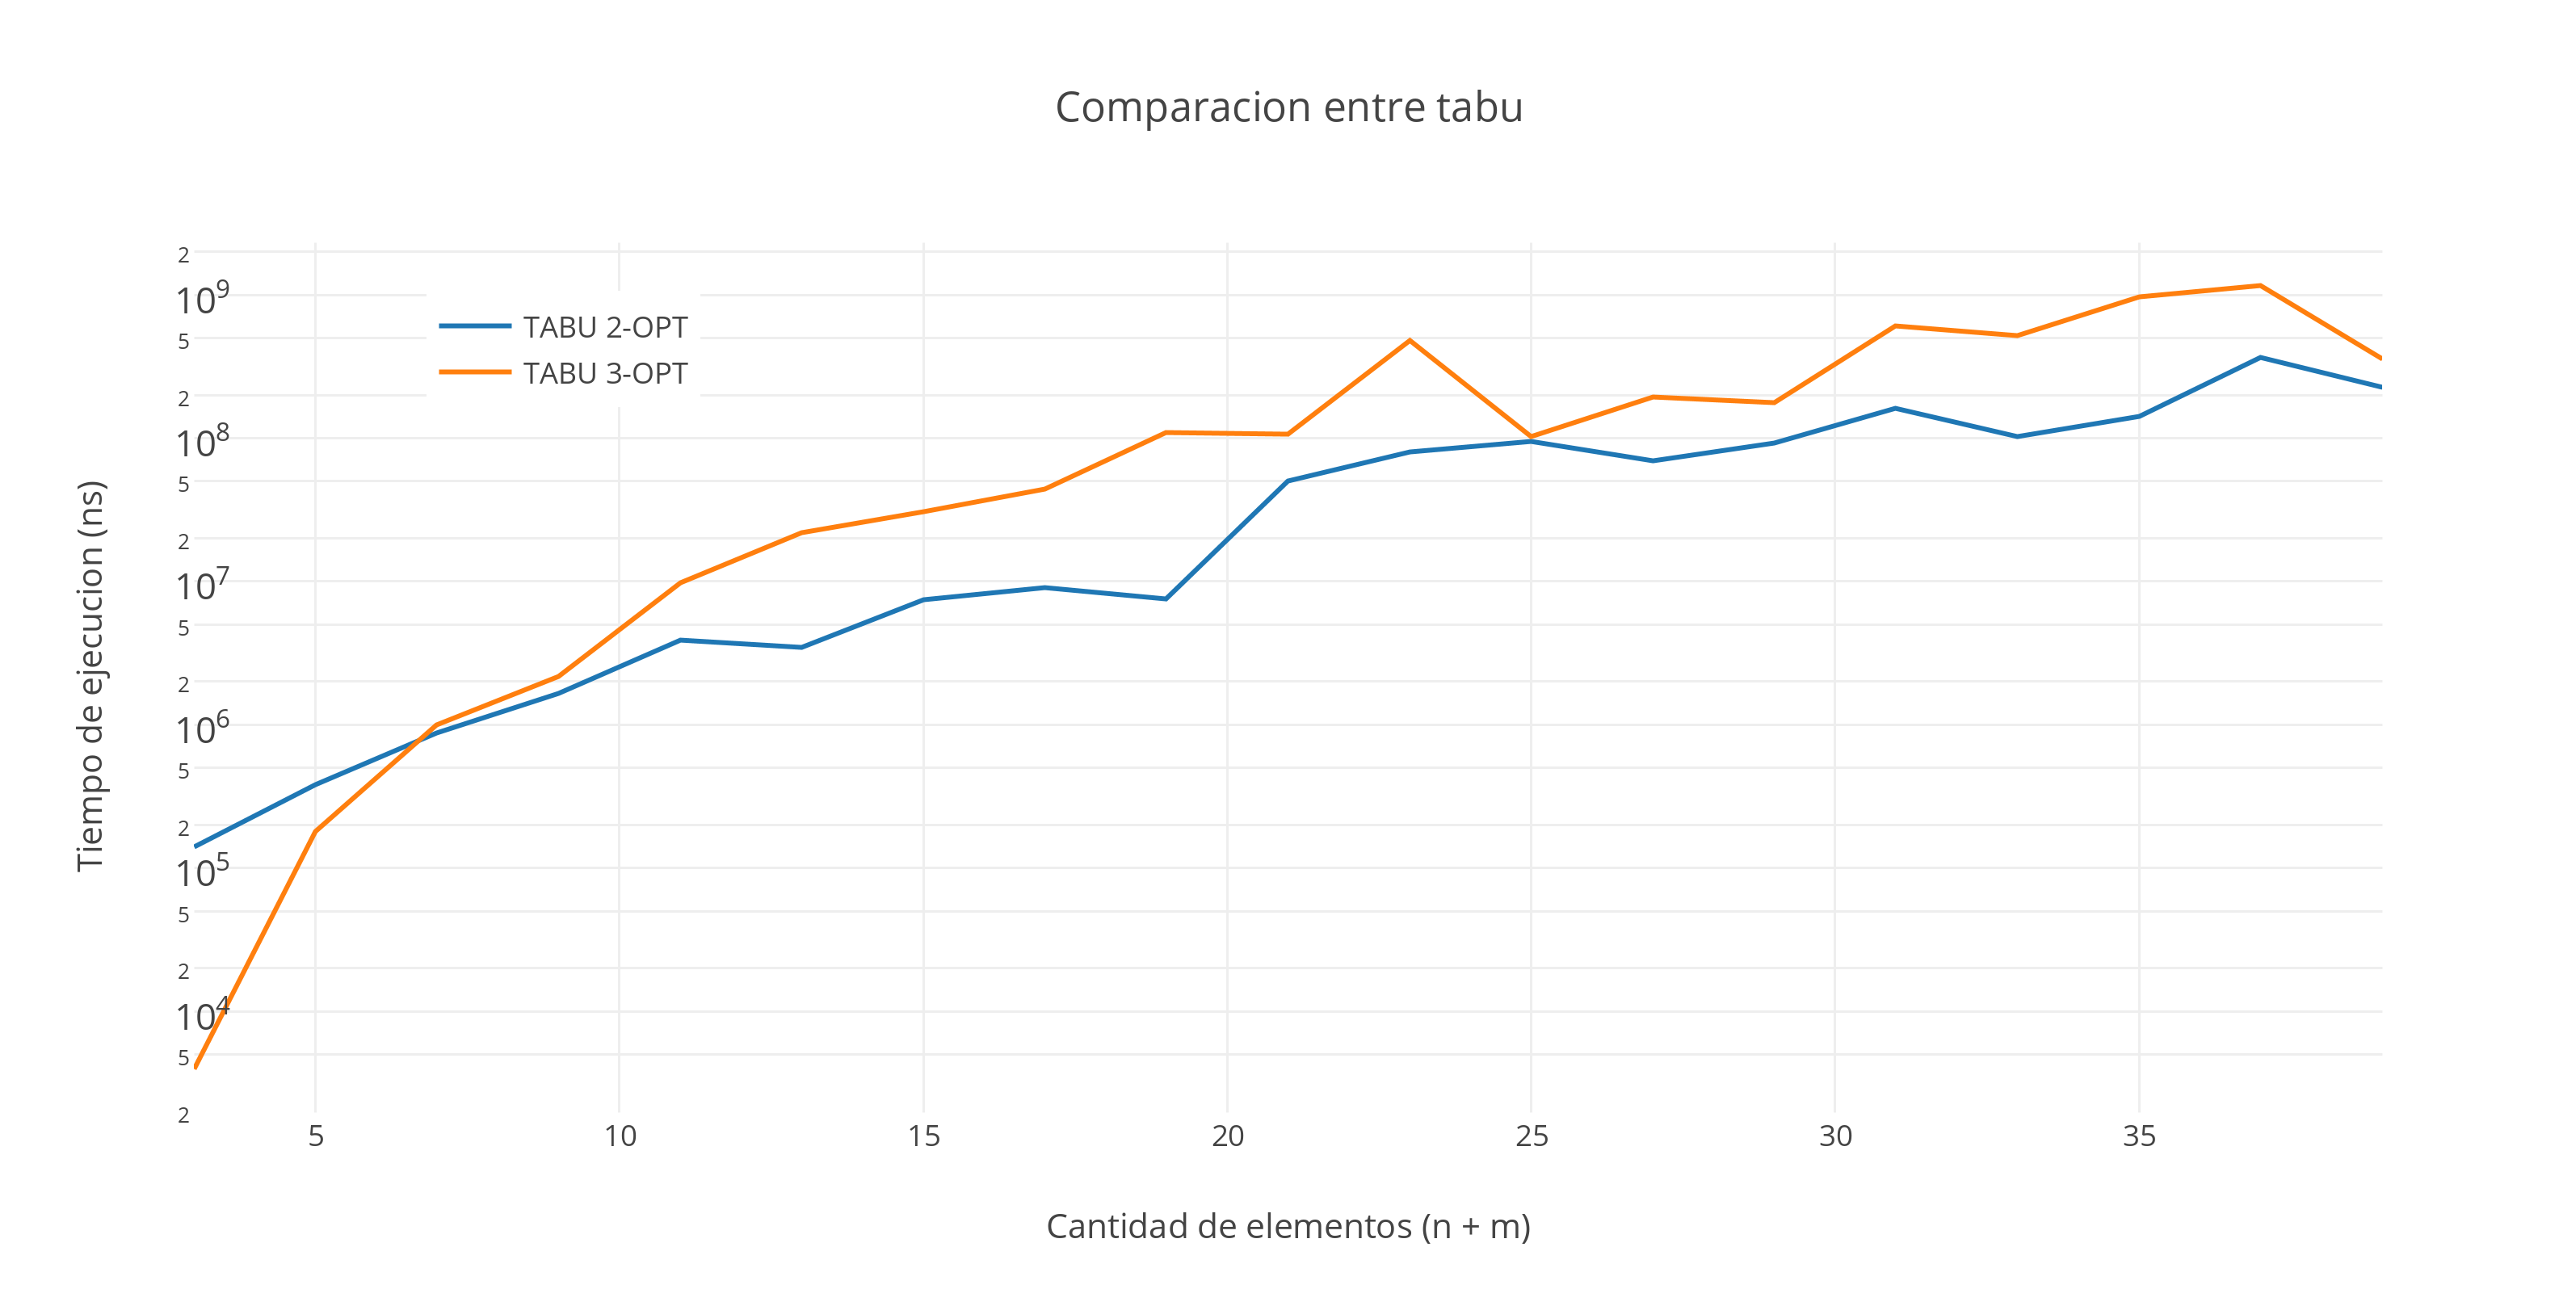
\includegraphics[scale=0.5]{./EJ4/comparaciongym01.png}\\
 {            \textit{Gráfico \ 4.6 - Tabu 2-OPT vs Tabu 3-OPT sobre Familia 4}}
  \end{center}
  \vspace*{0.3cm}

  
-----> HABLAR DE LA SOLUCION Q DA TABU 2-OPT Y 3-OPT CUAL SE MEJORO Y CUAL QUEDO IGUAL Y NO SERVIRIA USARLA EN ESTE CASO

\subsubsection*{Familia 6}


\vspace*{0.3cm} \vspace*{0.3cm}
  \begin{center}
 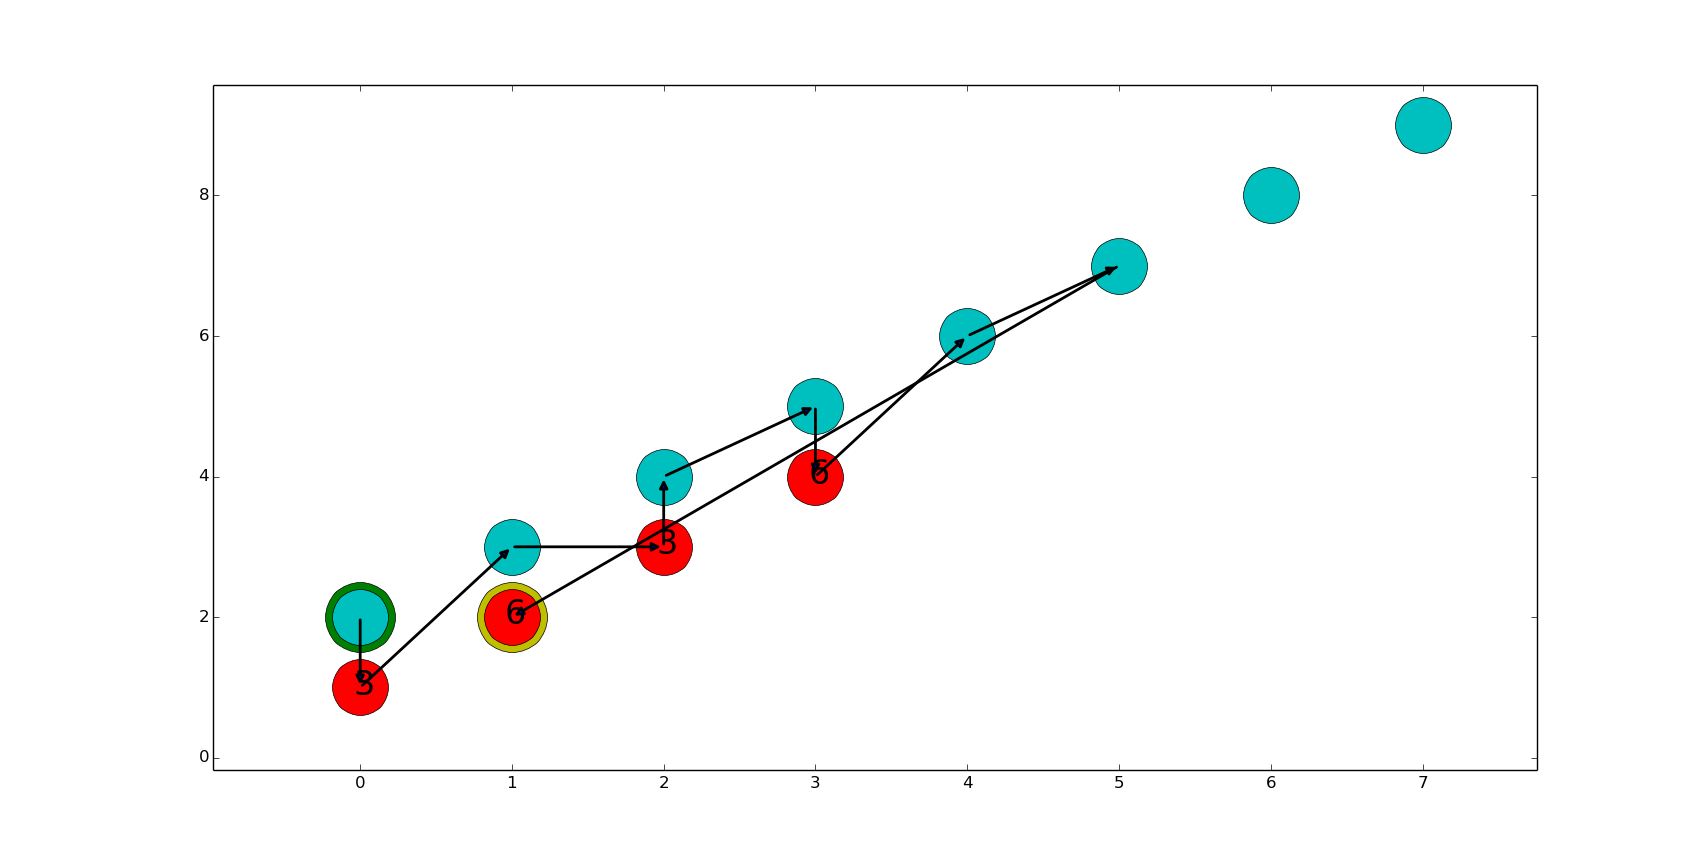
\includegraphics[scale=0.3]{./EJ4/fam6goloso.png}\\
 {            \textit{Soluci\'on Golosa}}
  \end{center}
  \vspace*{0.3cm}

\vspace*{0.3cm} \vspace*{0.3cm}
  \begin{center}
 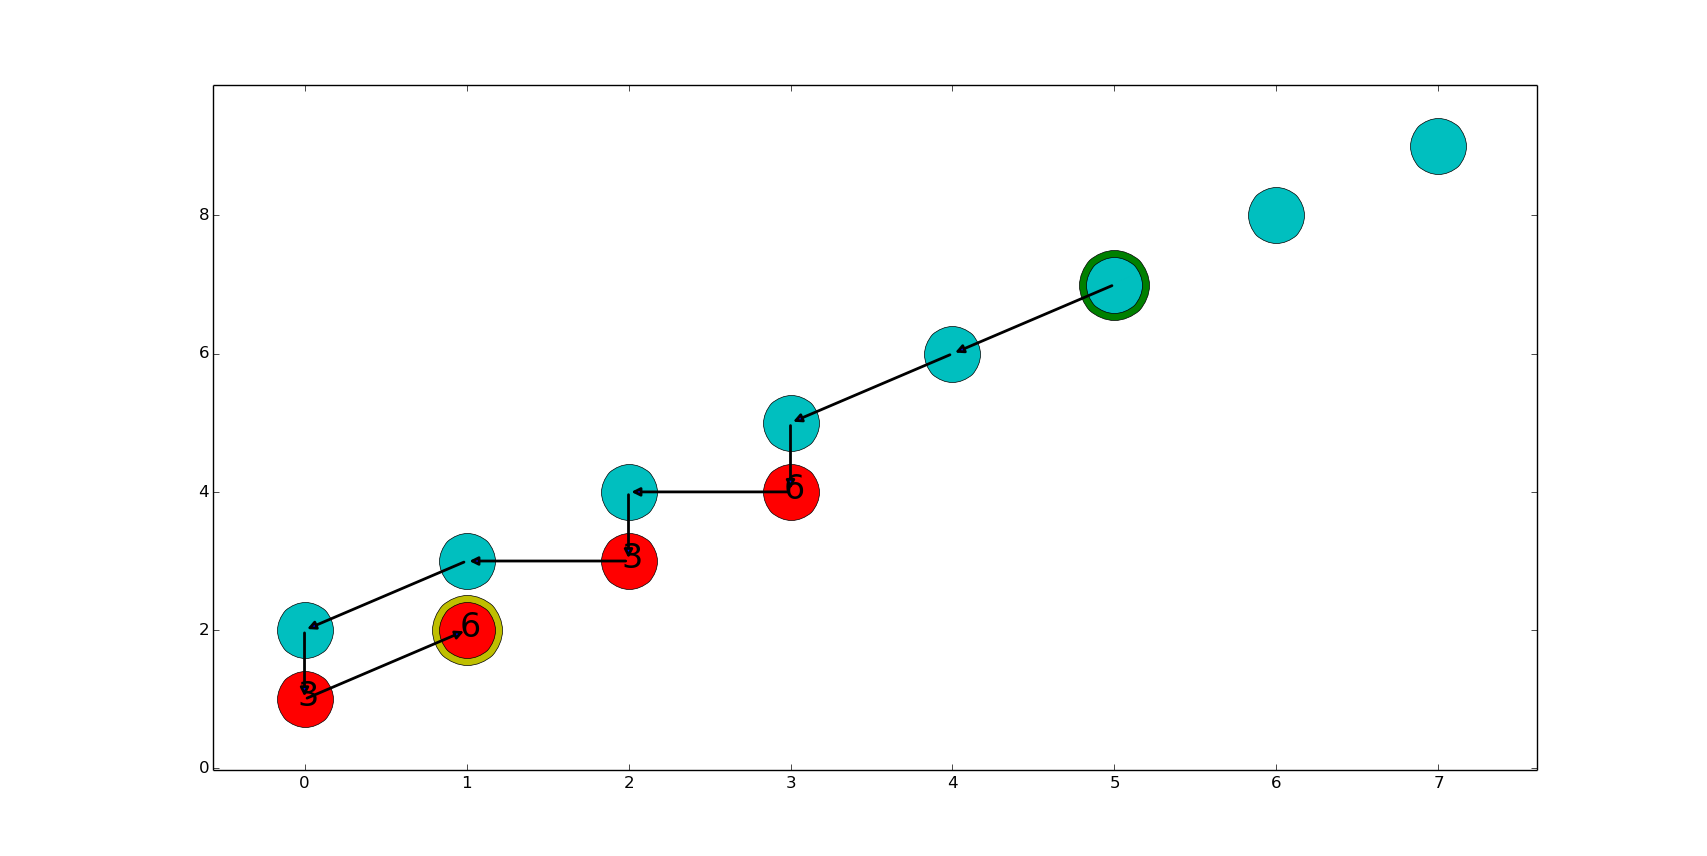
\includegraphics[scale=0.3]{./EJ4/fam62opt.png}\\
 {            \textit{Soluci\'on TABU 2-OPT}}
  \end{center}
  \vspace*{0.3cm}

\vspace*{0.3cm} \vspace*{0.3cm}
  \begin{center}
 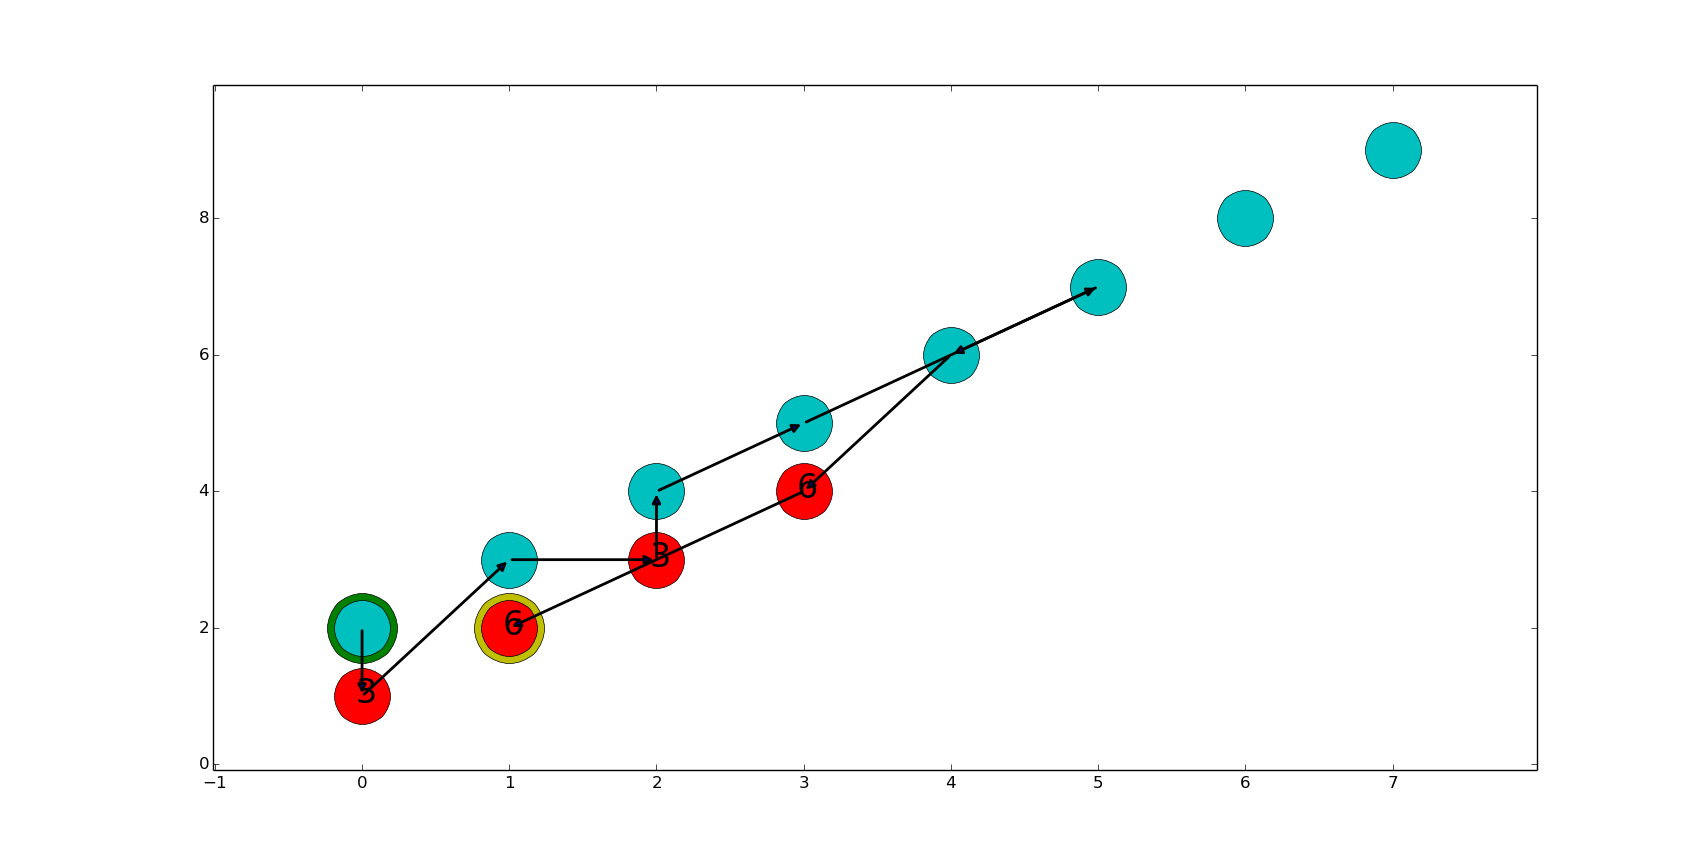
\includegraphics[scale=0.3]{./EJ4/fam63opt.png}\\
 {            \textit{Soluci\'on TABU 3-OPT}}
  \end{center}
  \vspace*{0.3cm}

-----> ACOMODARLO

Veamos como se comporta Tabu 2-OPT con respecto a la heuristica de busqueda local 2-OPT:

\vspace*{0.3cm} \vspace*{0.3cm}
  \begin{center}
 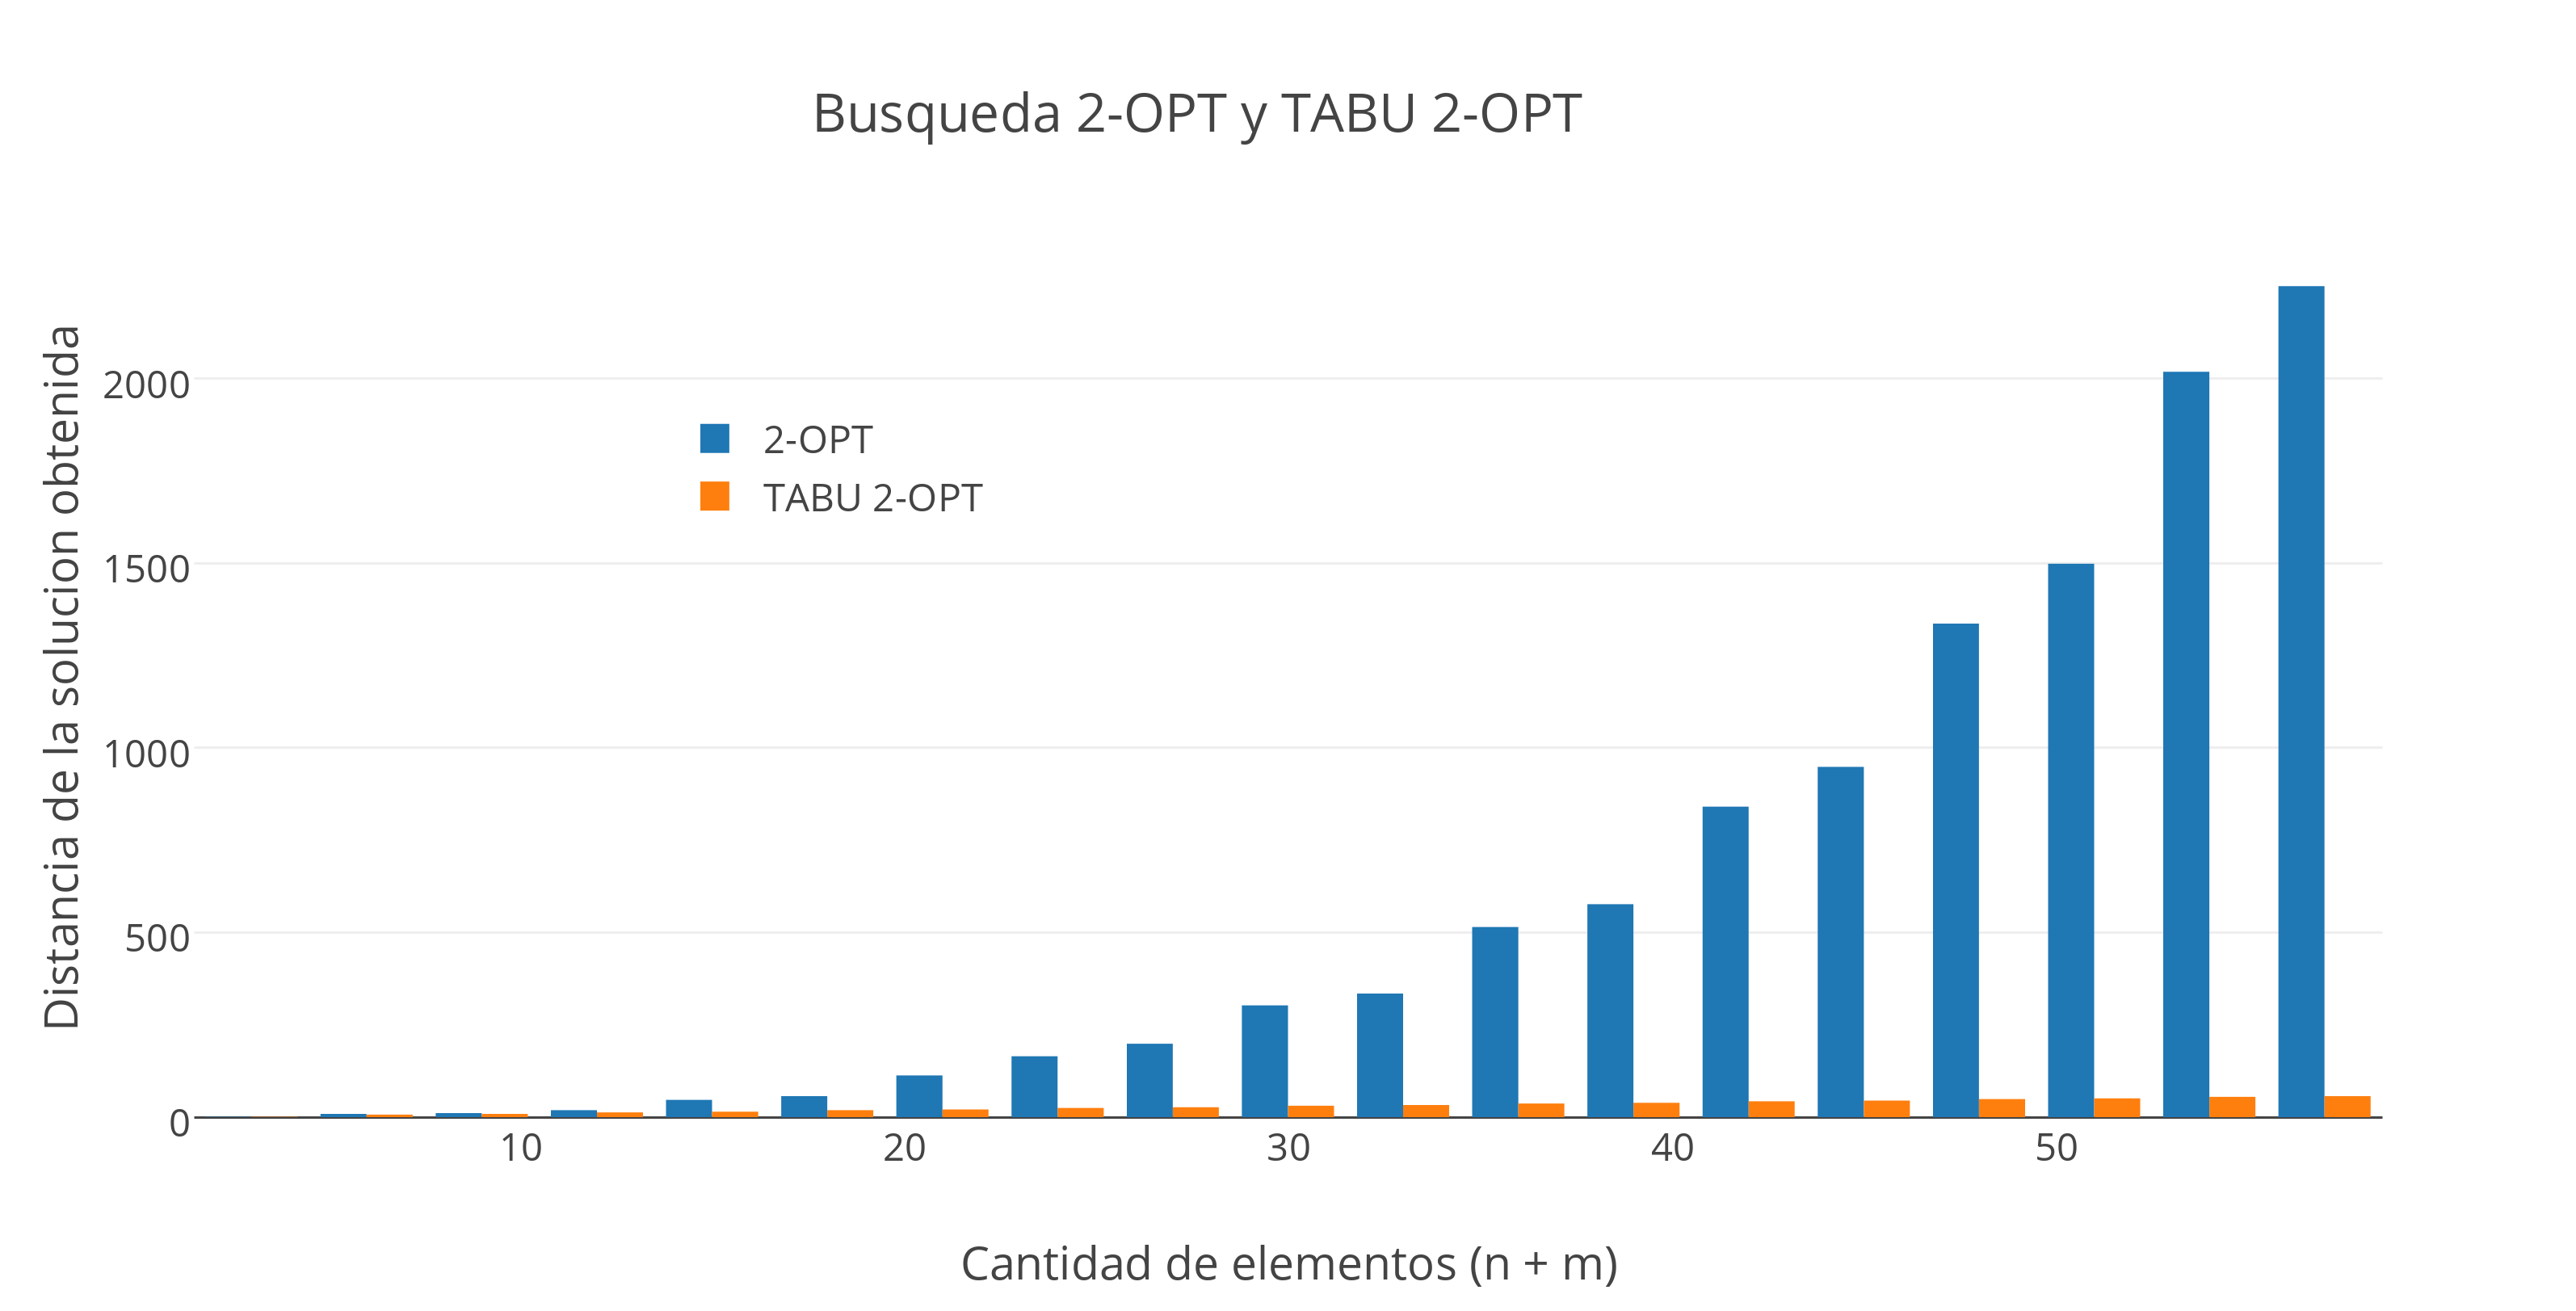
\includegraphics[scale=0.5]{./EJ4/comparativosinorden2opt.png}\\
 {            \textit{Gráfico \ 4.7 - 2-OPT vs Tabu 2-OPT sobre Familia 6}}
  \end{center}
  \vspace*{0.3cm}

En cuanto a tiempo insumido vemos lo siguiente:

\vspace*{0.3cm} \vspace*{0.3cm}
  \begin{center}
 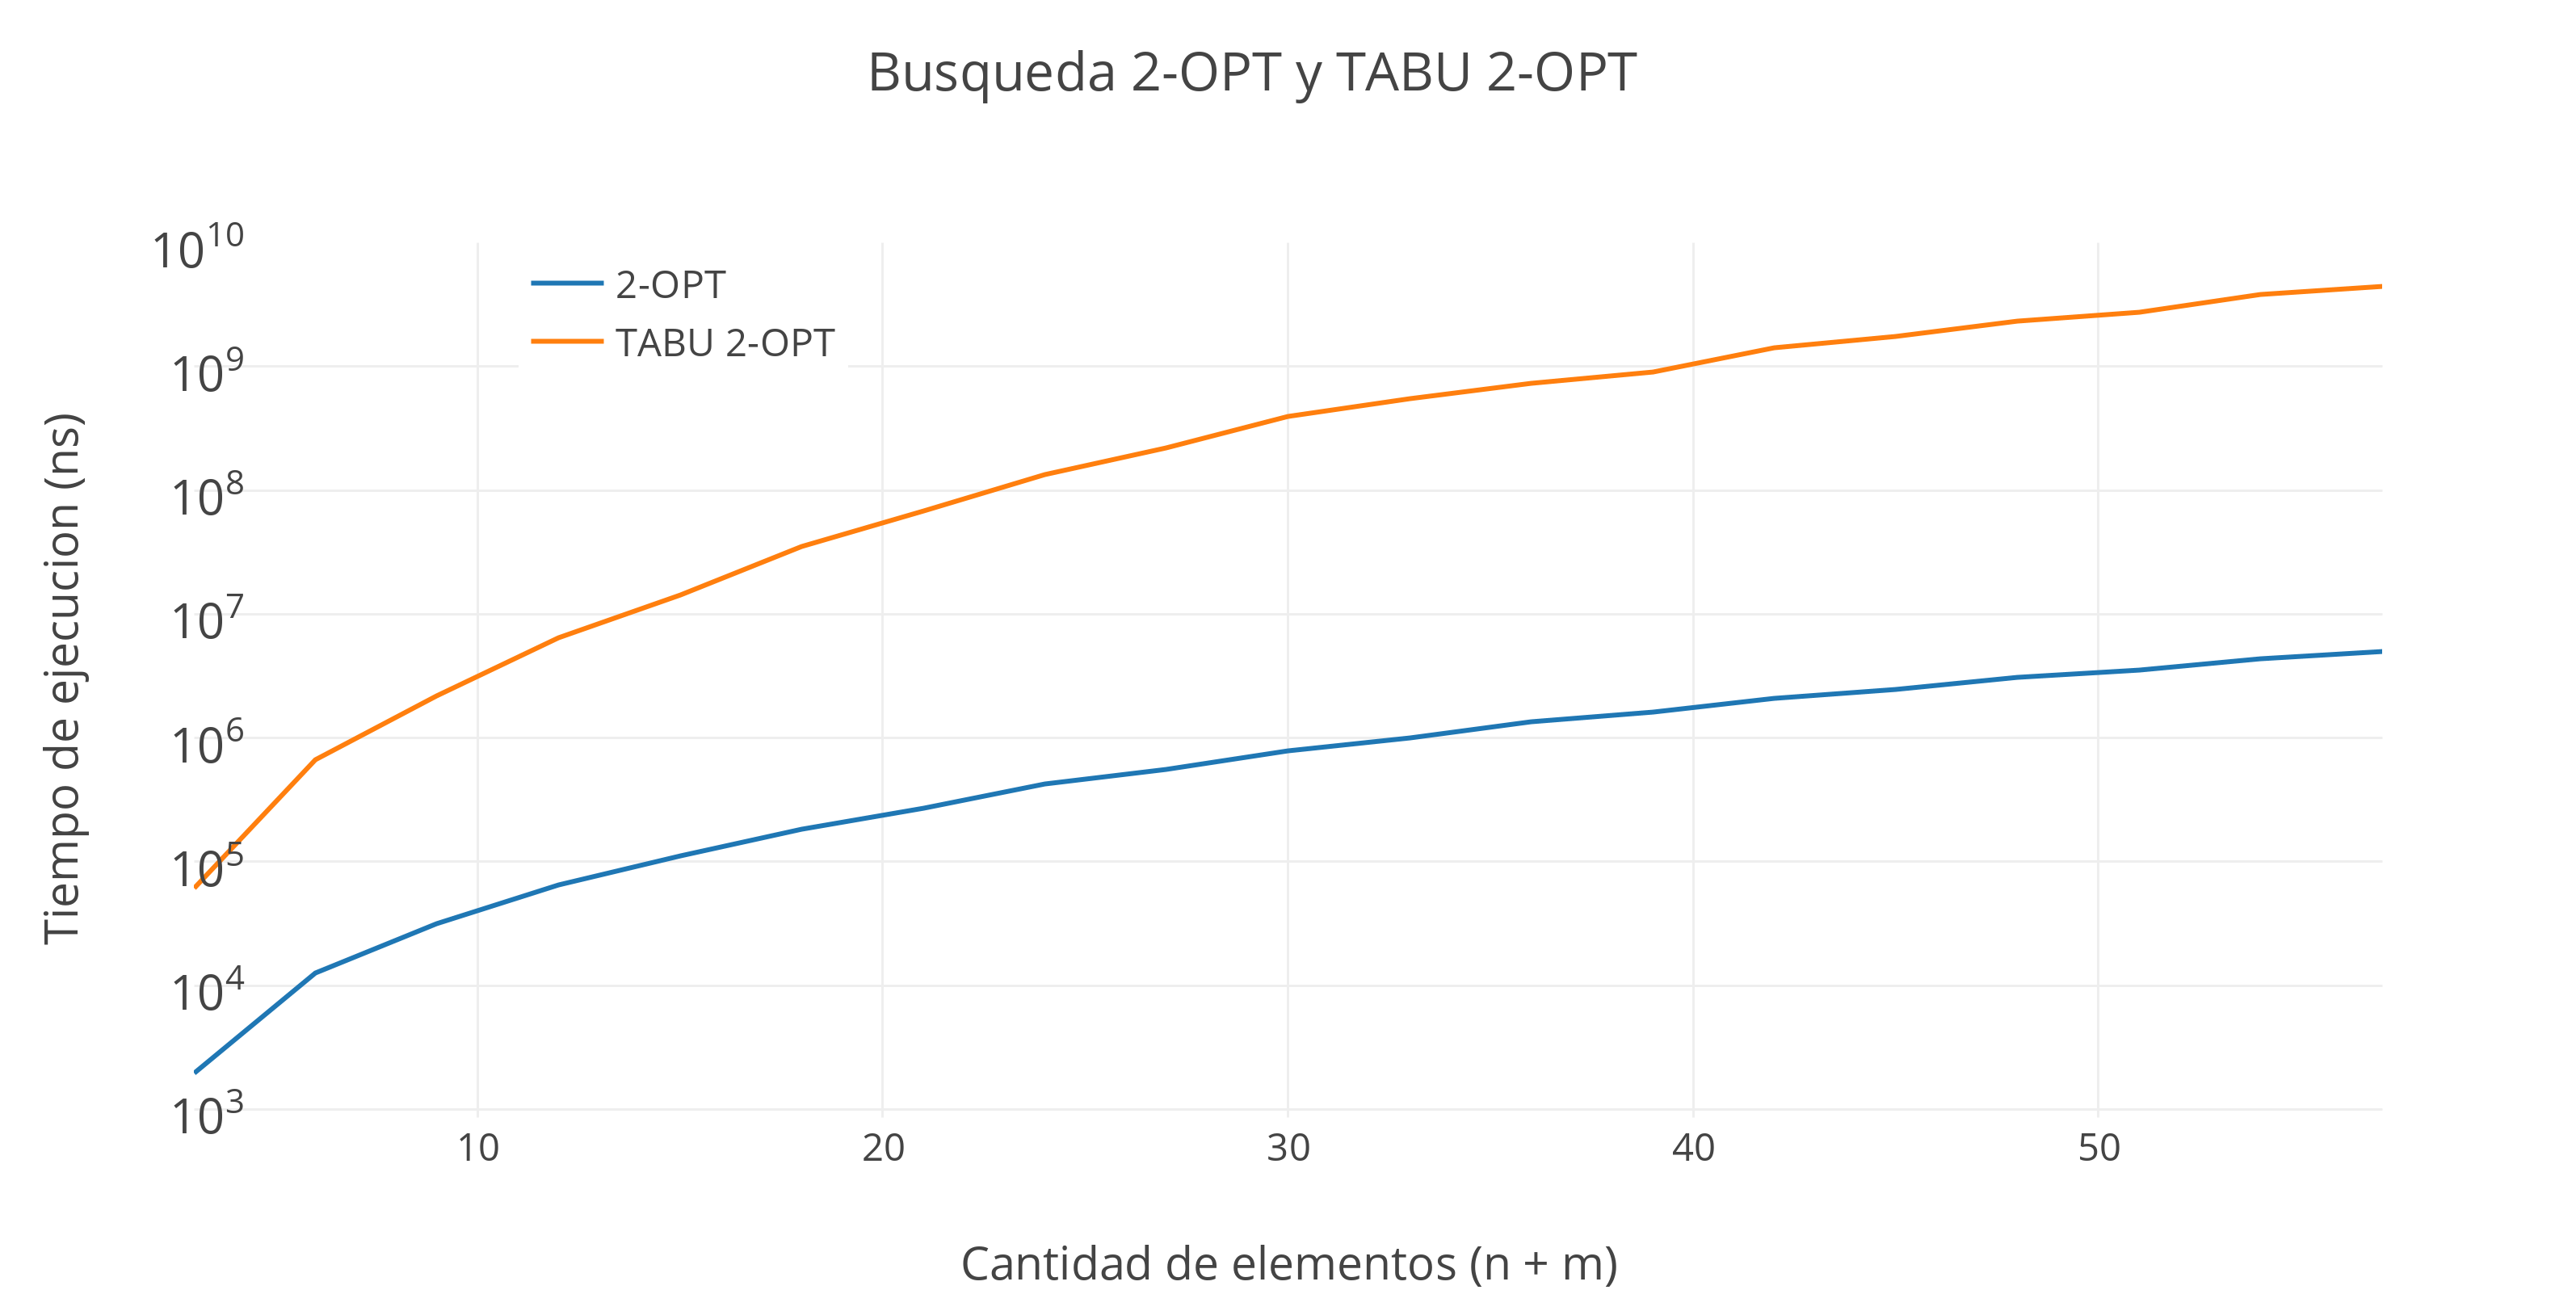
\includegraphics[scale=0.5]{./EJ4/medicion2optsinorden.png}\\
 {            \textit{Gráfico \ 4.8 - 2-OPT vs Tabu 2-OPT sobre Familia 6}}
  \end{center}
  \vspace*{0.3cm}


Luego, para 3-OPT:

\vspace*{0.3cm} \vspace*{0.3cm}
  \begin{center}
 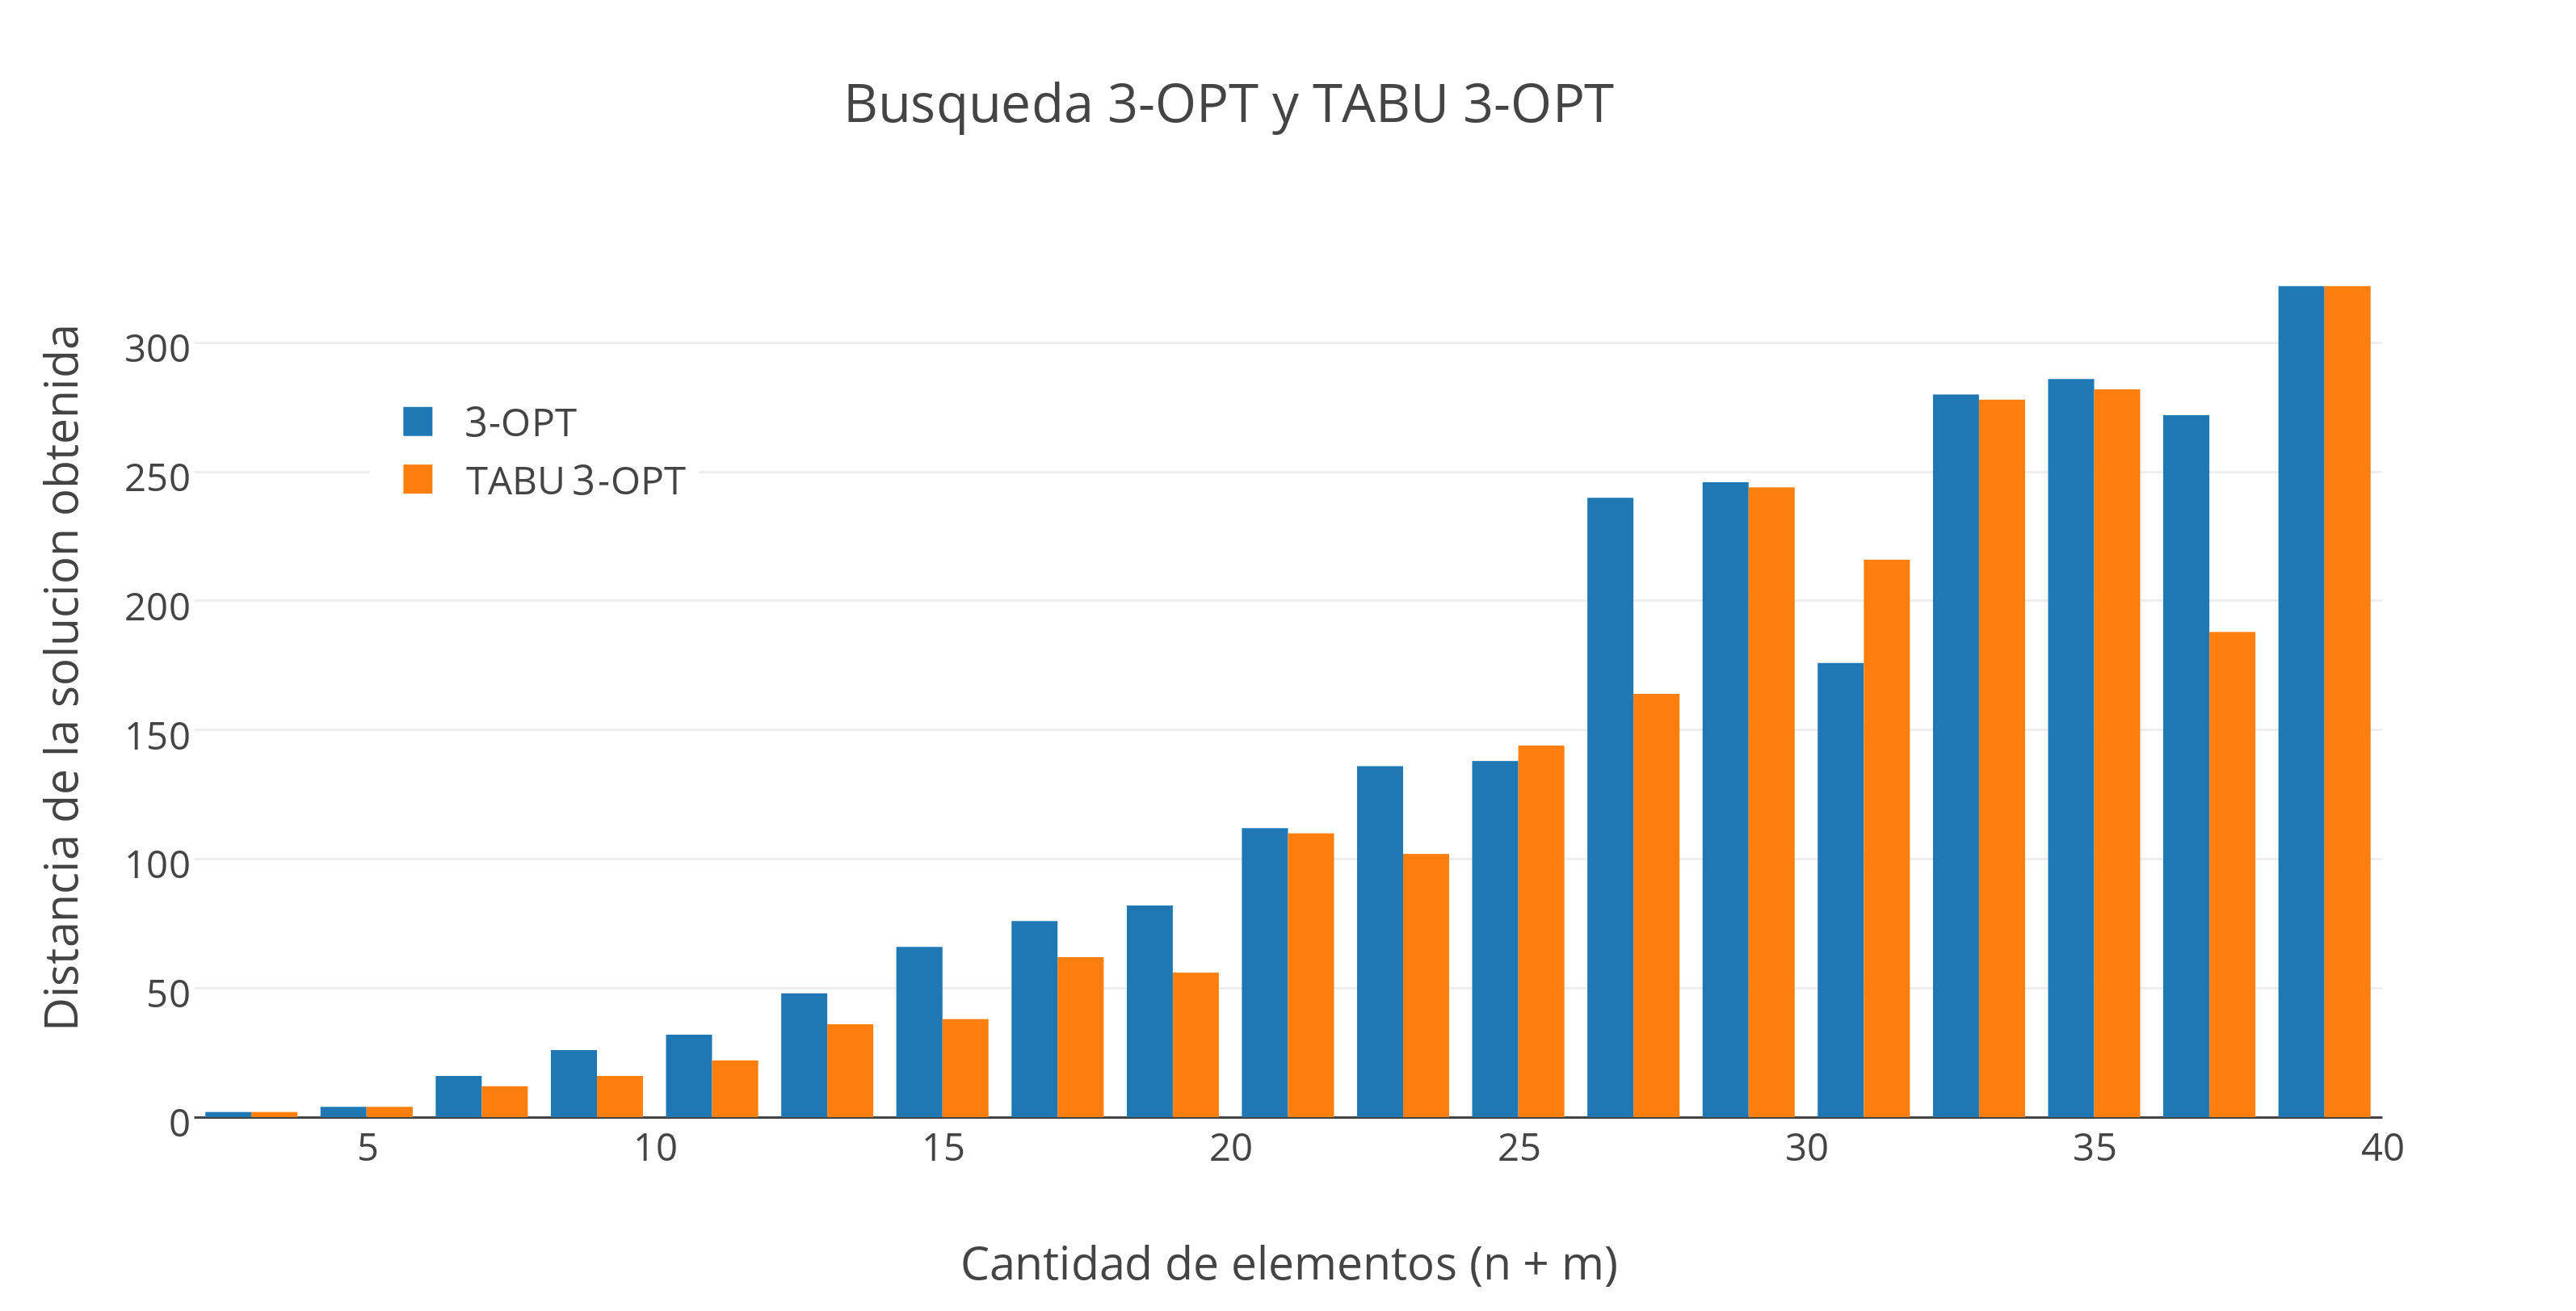
\includegraphics[scale=0.5]{./EJ4/comparativogym03opt.png}\\
 {            \textit{Gráfico \ 4.9 - 3-OPT vs Tabu 3-OPT sobre Familia 6}}
  \end{center}
  \vspace*{0.3cm}

En cuanto a tiempo insumido vemos lo siguiente:

\vspace*{0.3cm} \vspace*{0.3cm}
  \begin{center}
 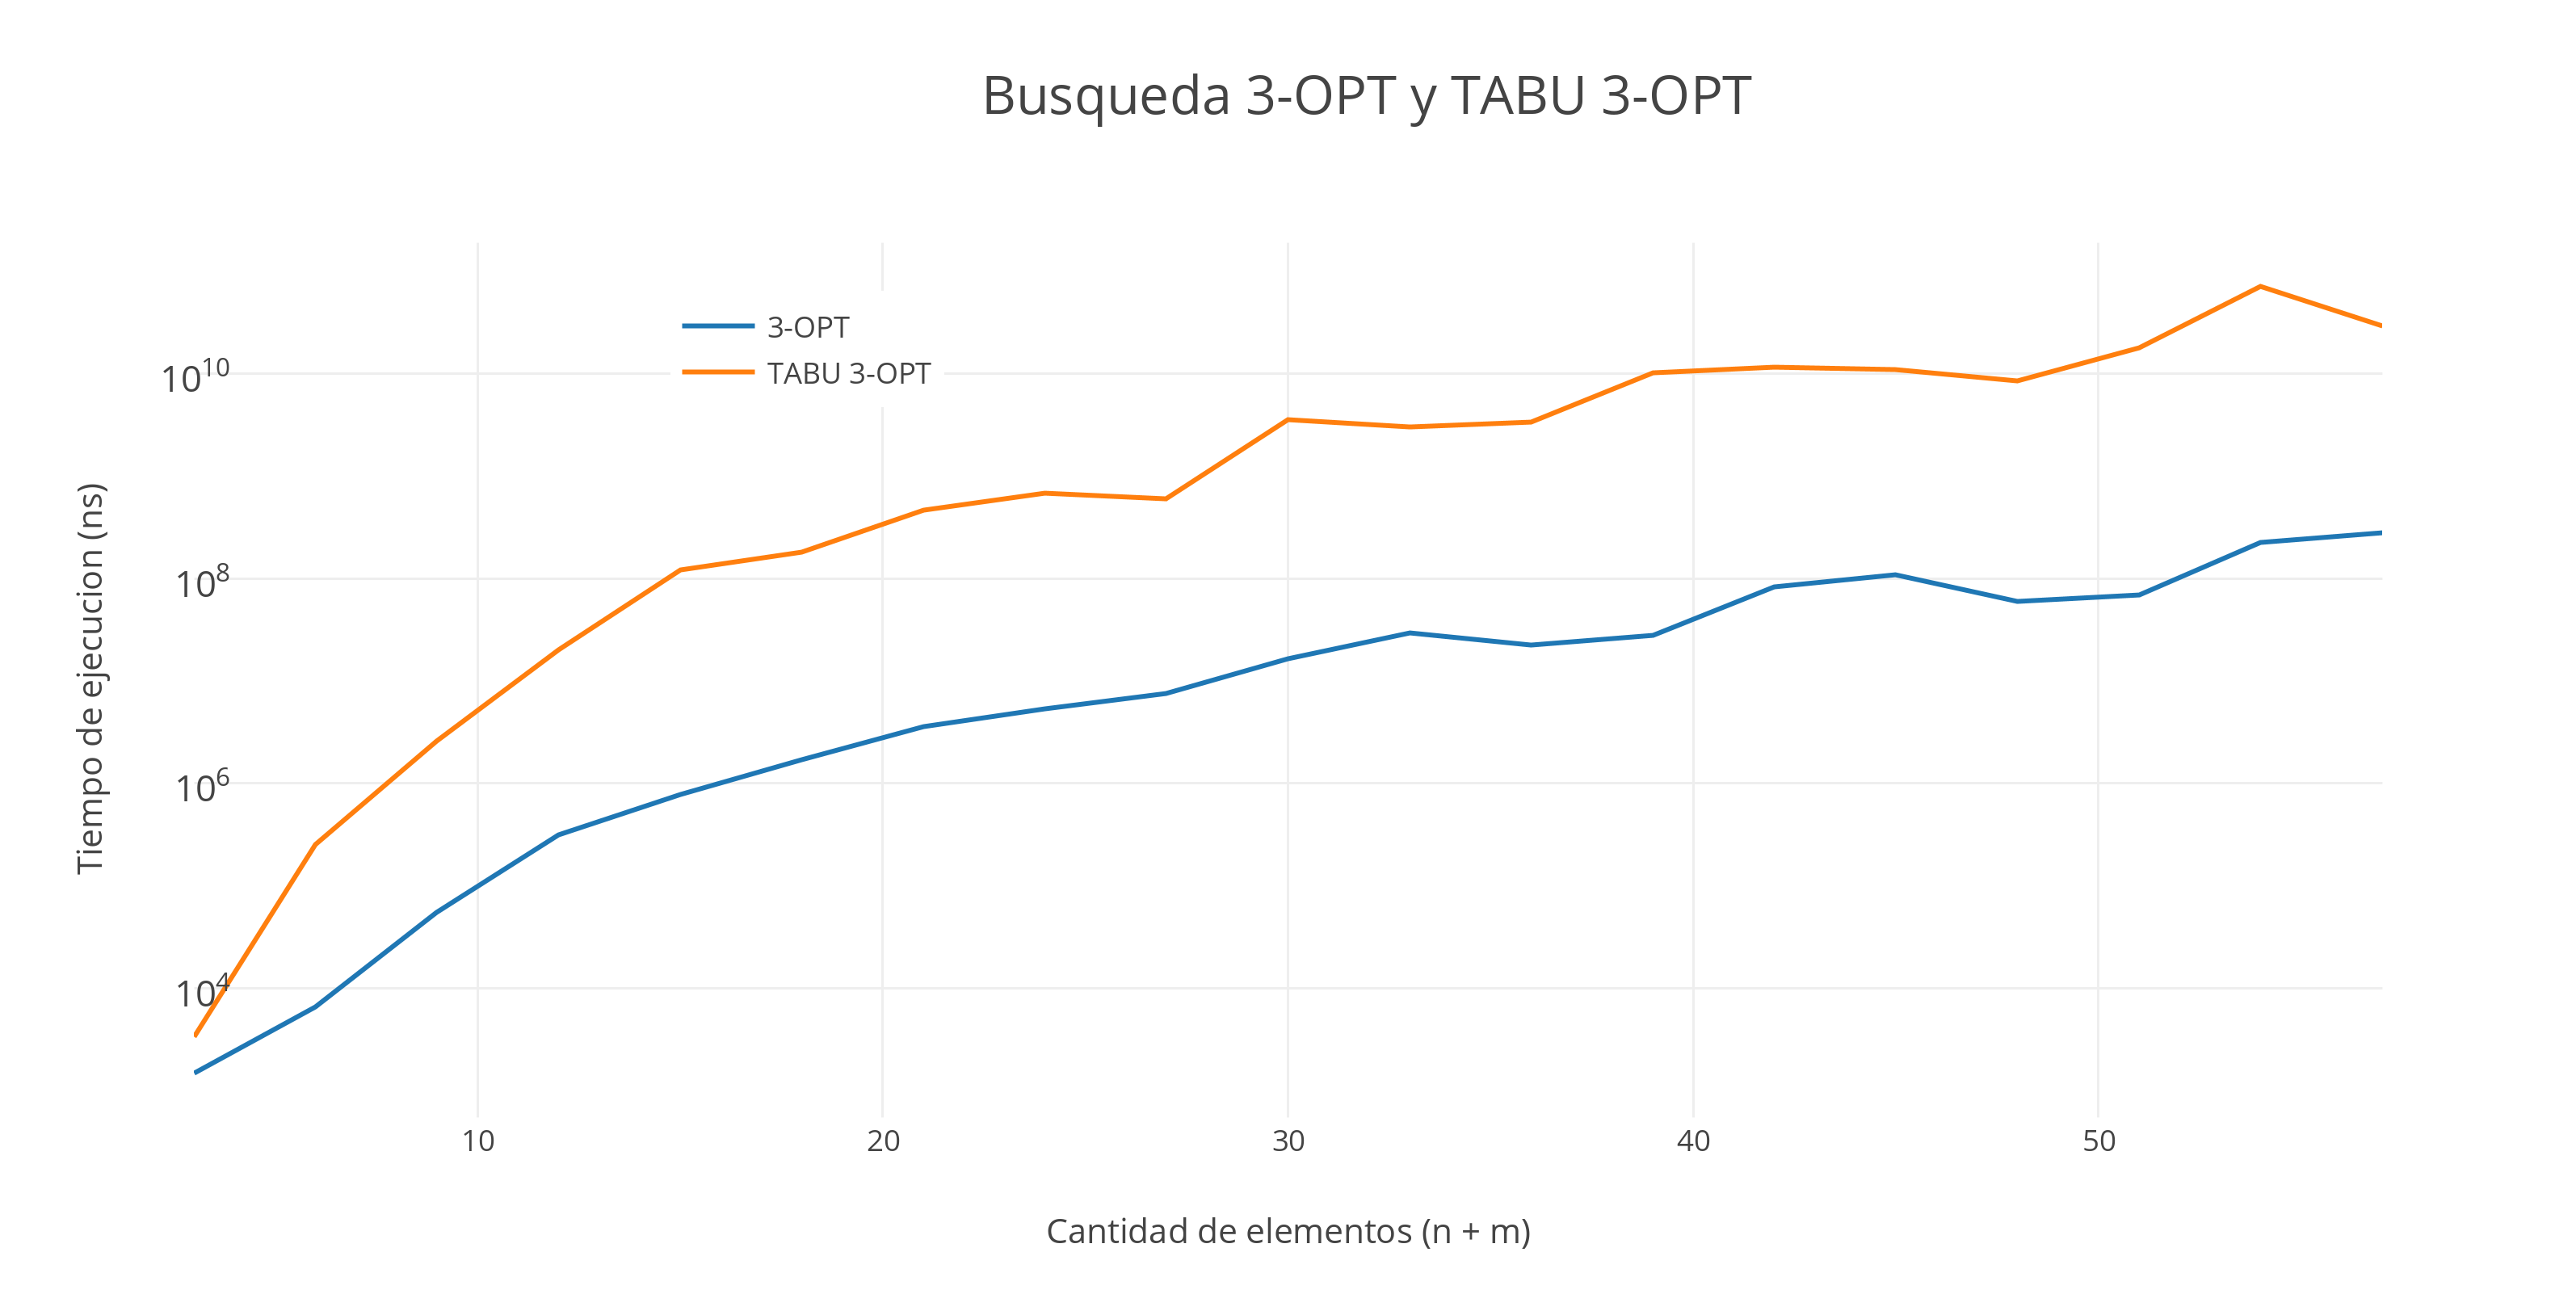
\includegraphics[scale=0.5]{./EJ4/medicion3optsinorden.png}\\
 {            \textit{Gráfico \ 4.10 - 3-OPT vs Tabu 3-OPT sobre Familia 6}}
  \end{center}
  \vspace*{0.3cm}
  
Para la comparación entre algoritmos tabu, se comparará conjuntamente el tiempo de ejecución con la calidad de la solución. Para esta última tendremos en cuenta que los algoritmos, de devolver un resultado, será válido: esto quiere decir que cuanto menor distancia recorran en las soluciones, mejor serán las mismas:

Las soluciones obtenidas fueron las siguientes:

\vspace*{0.3cm} \vspace*{0.3cm}
  \begin{center}
 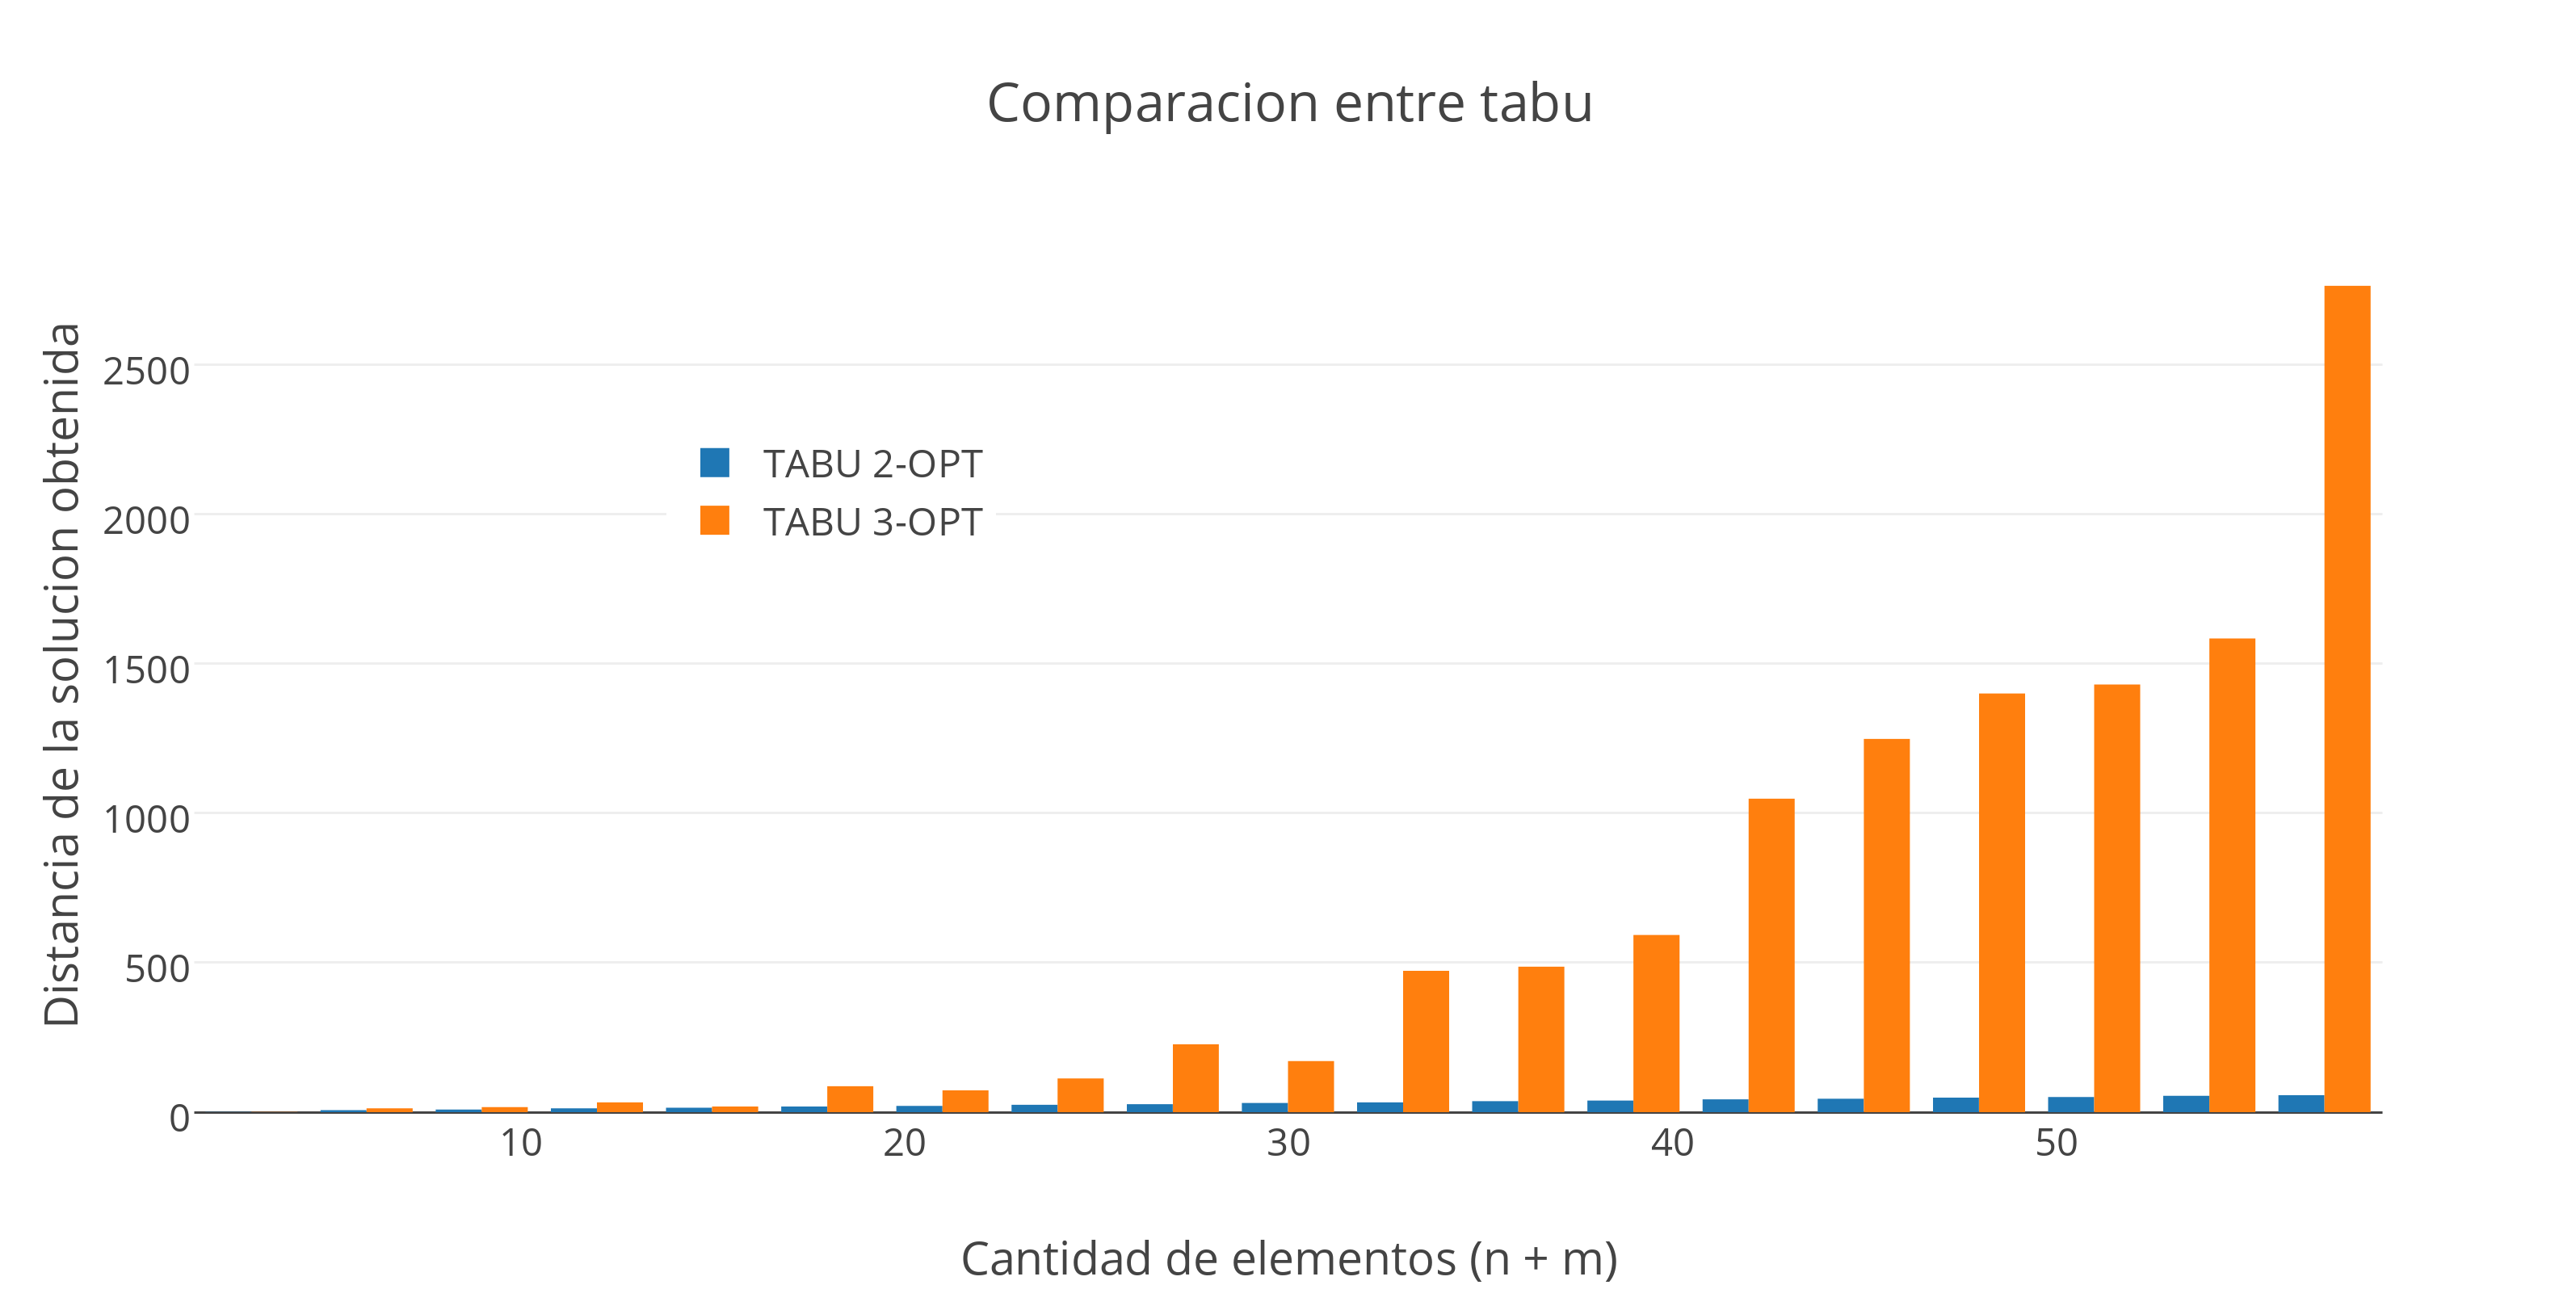
\includegraphics[scale=0.5]{./EJ4/comparativosinorden.png}\\
 {            \textit{Gráfico \ 4.11 - Tabu 2-OPT vs Tabu 3-OPT sobre Familia 6}}
  \end{center}
  \vspace*{0.3cm}

En cuanto a tiempo insumido vemos lo siguiente:

\vspace*{0.3cm} \vspace*{0.3cm}
  \begin{center}
 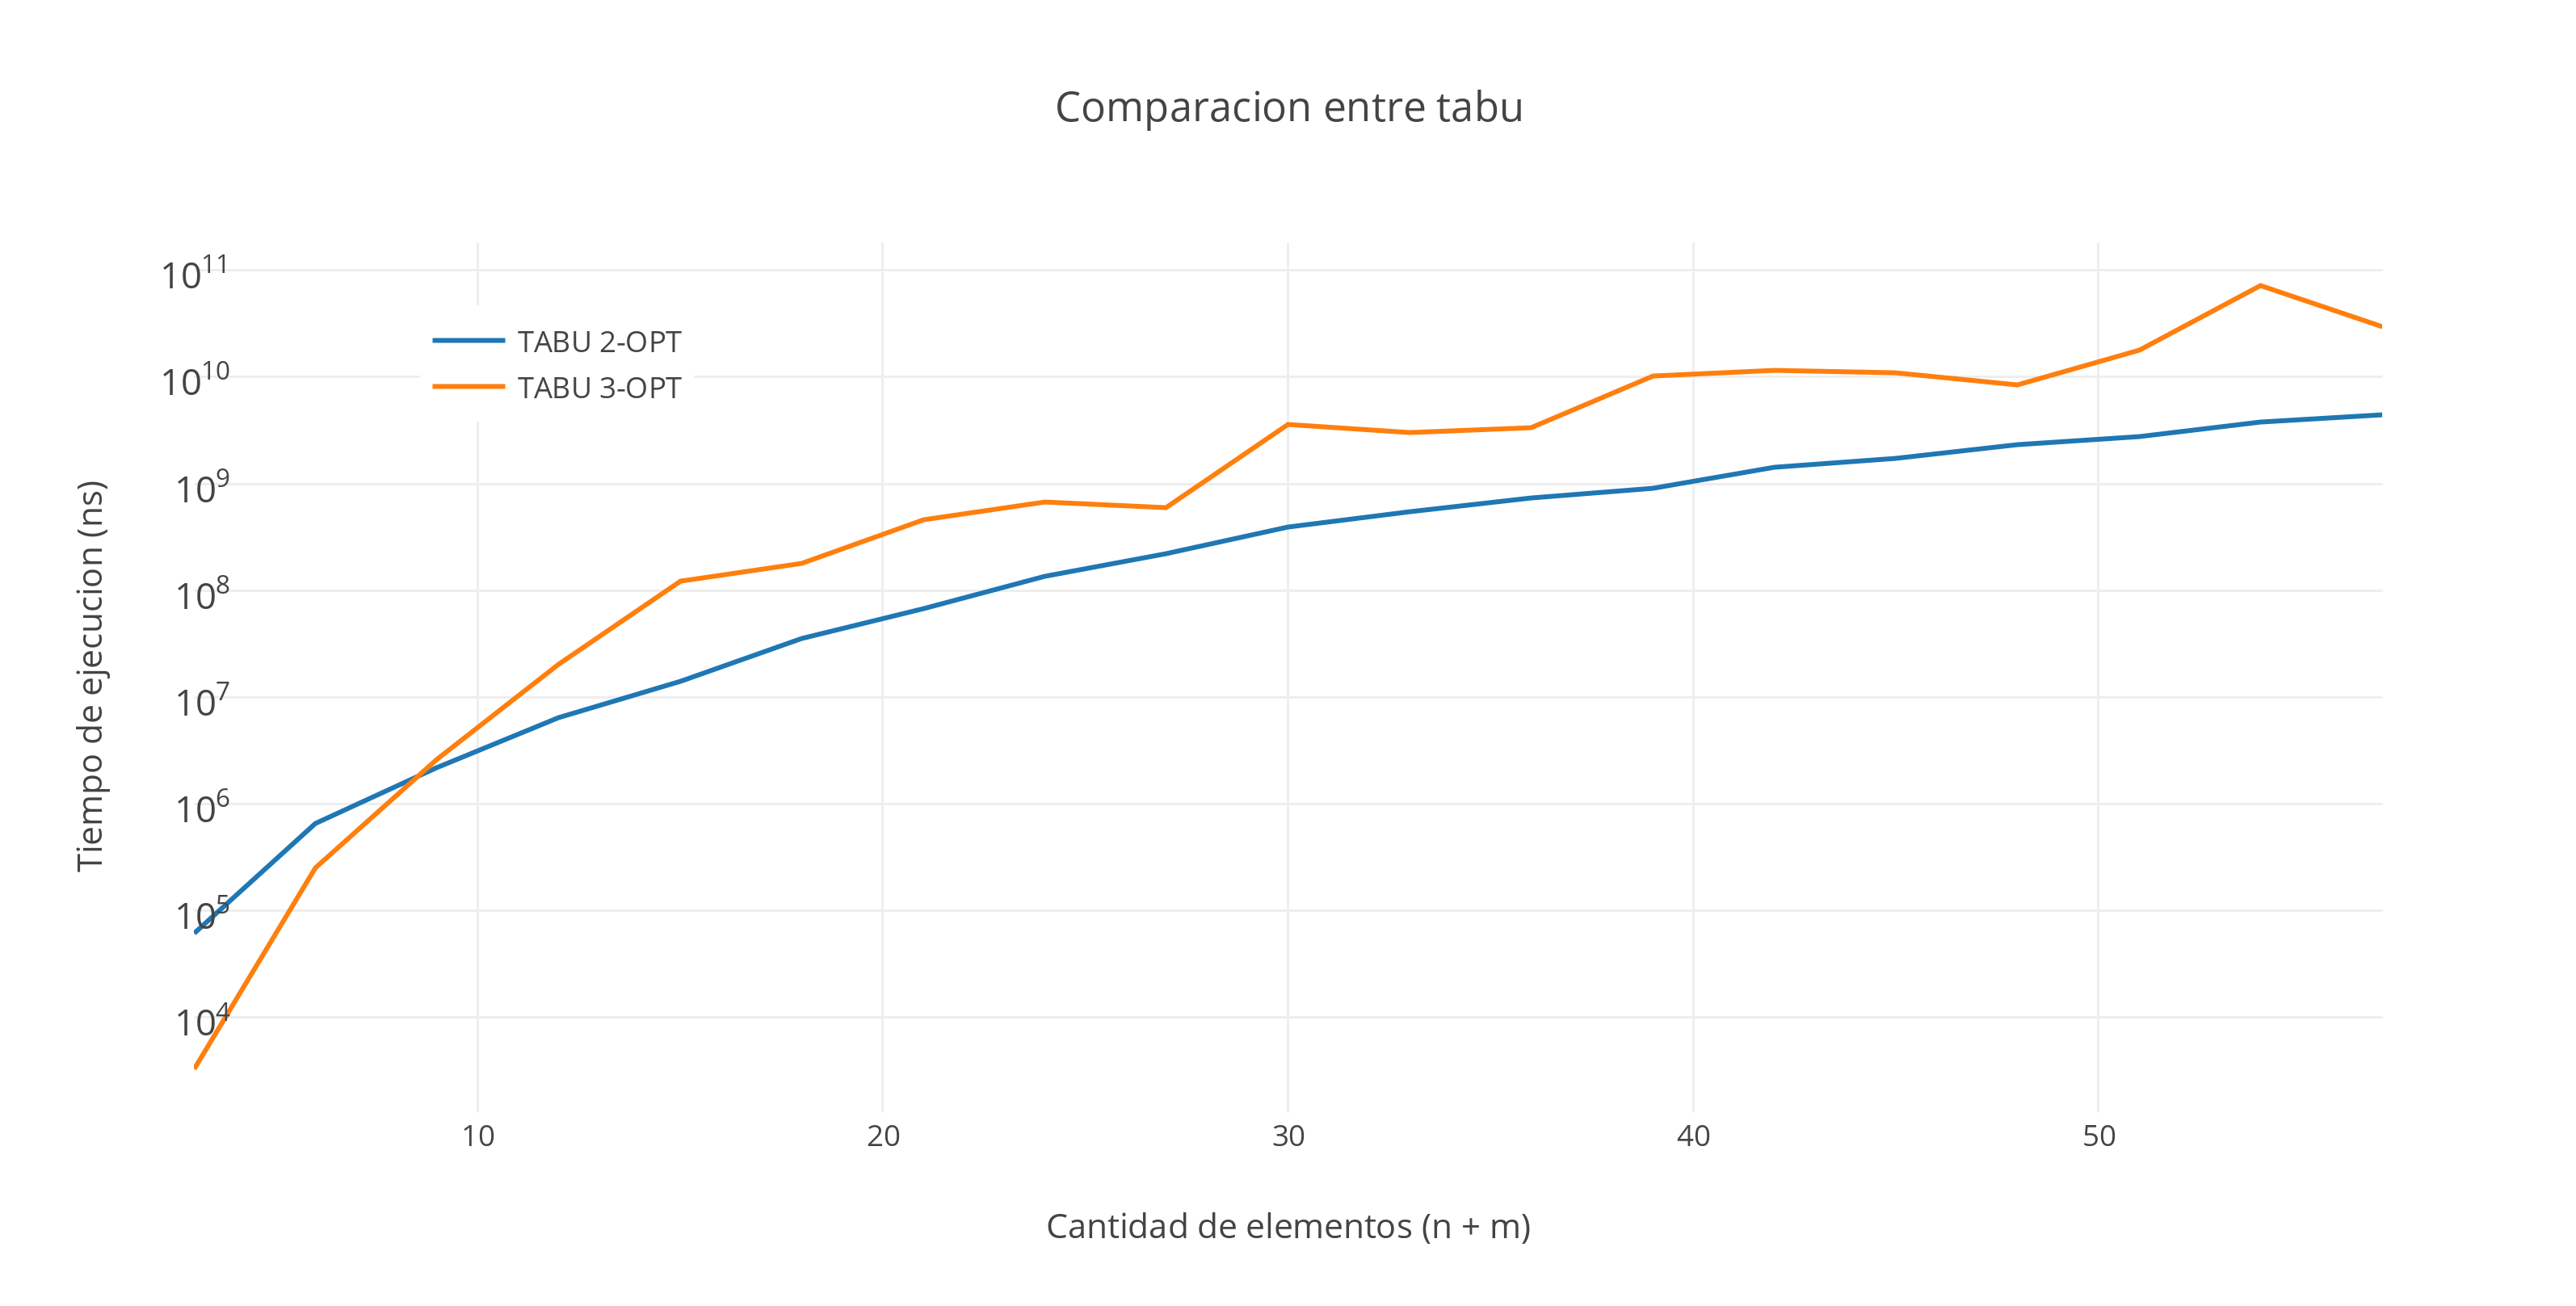
\includegraphics[scale=0.5]{./EJ4/comparacionsinorden1.png}\\
 {            \textit{Gráfico \ 4.12 - Tabu 2-OPT vs Tabu 3-OPT sobre Familia 6}}
  \end{center}
  \vspace*{0.3cm}




\subsubsection*{Familia 7}


\vspace*{0.3cm} \vspace*{0.3cm}
  \begin{center}
 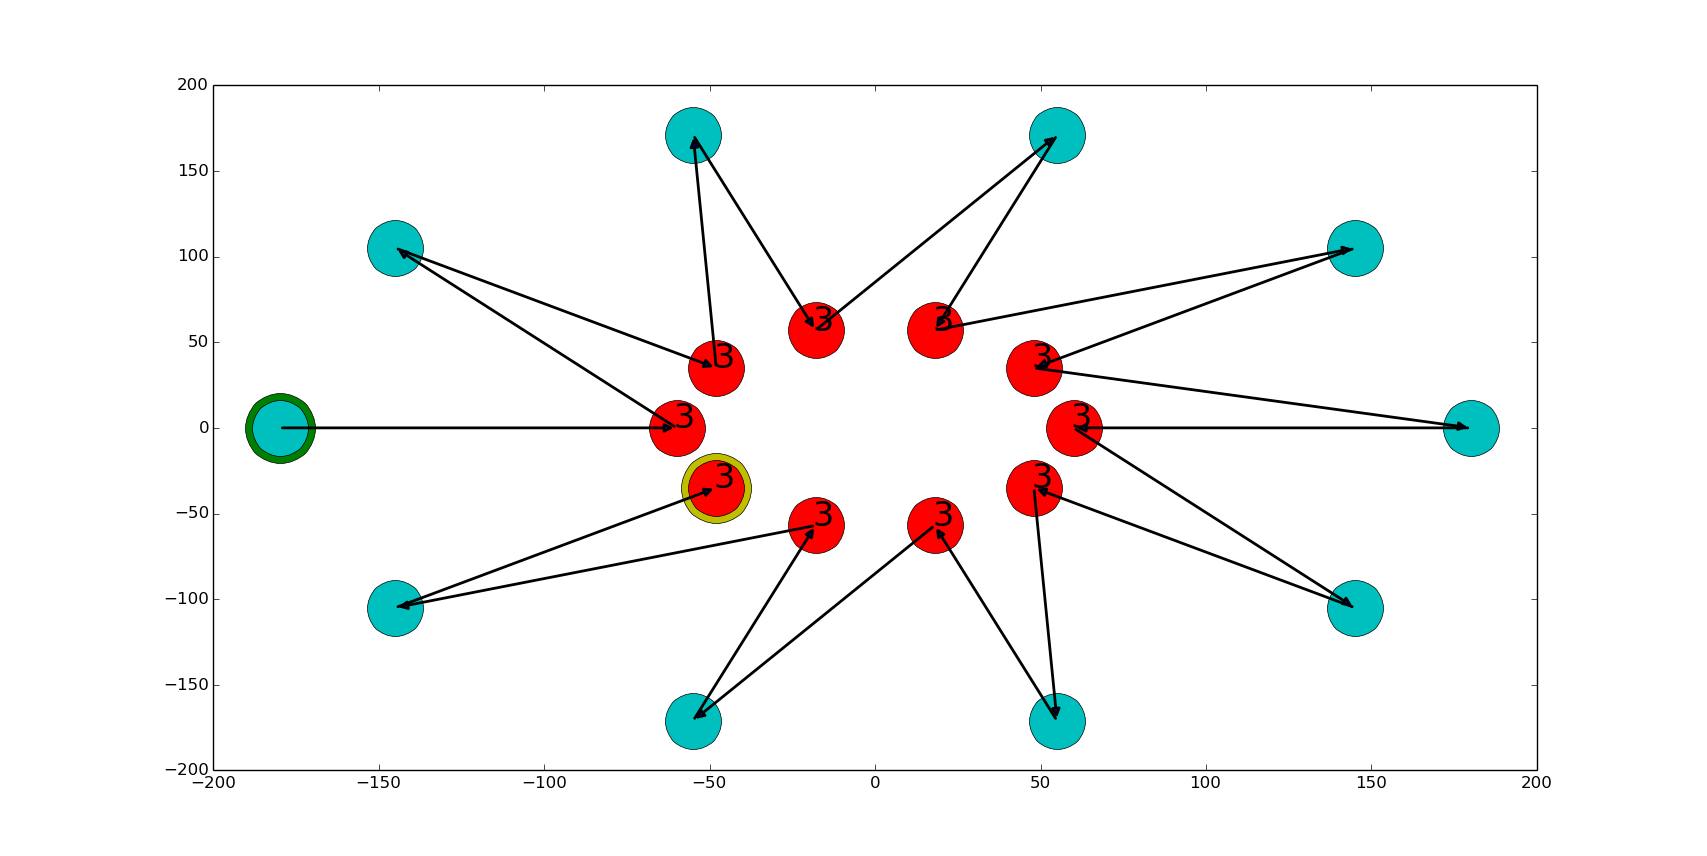
\includegraphics[scale=0.3]{./EJ4/fam7goloso.png}\\
 {            \textit{Soluci\'on Golosa}}
  \end{center}
  \vspace*{0.3cm}

\vspace*{0.3cm} \vspace*{0.3cm}
  \begin{center}
 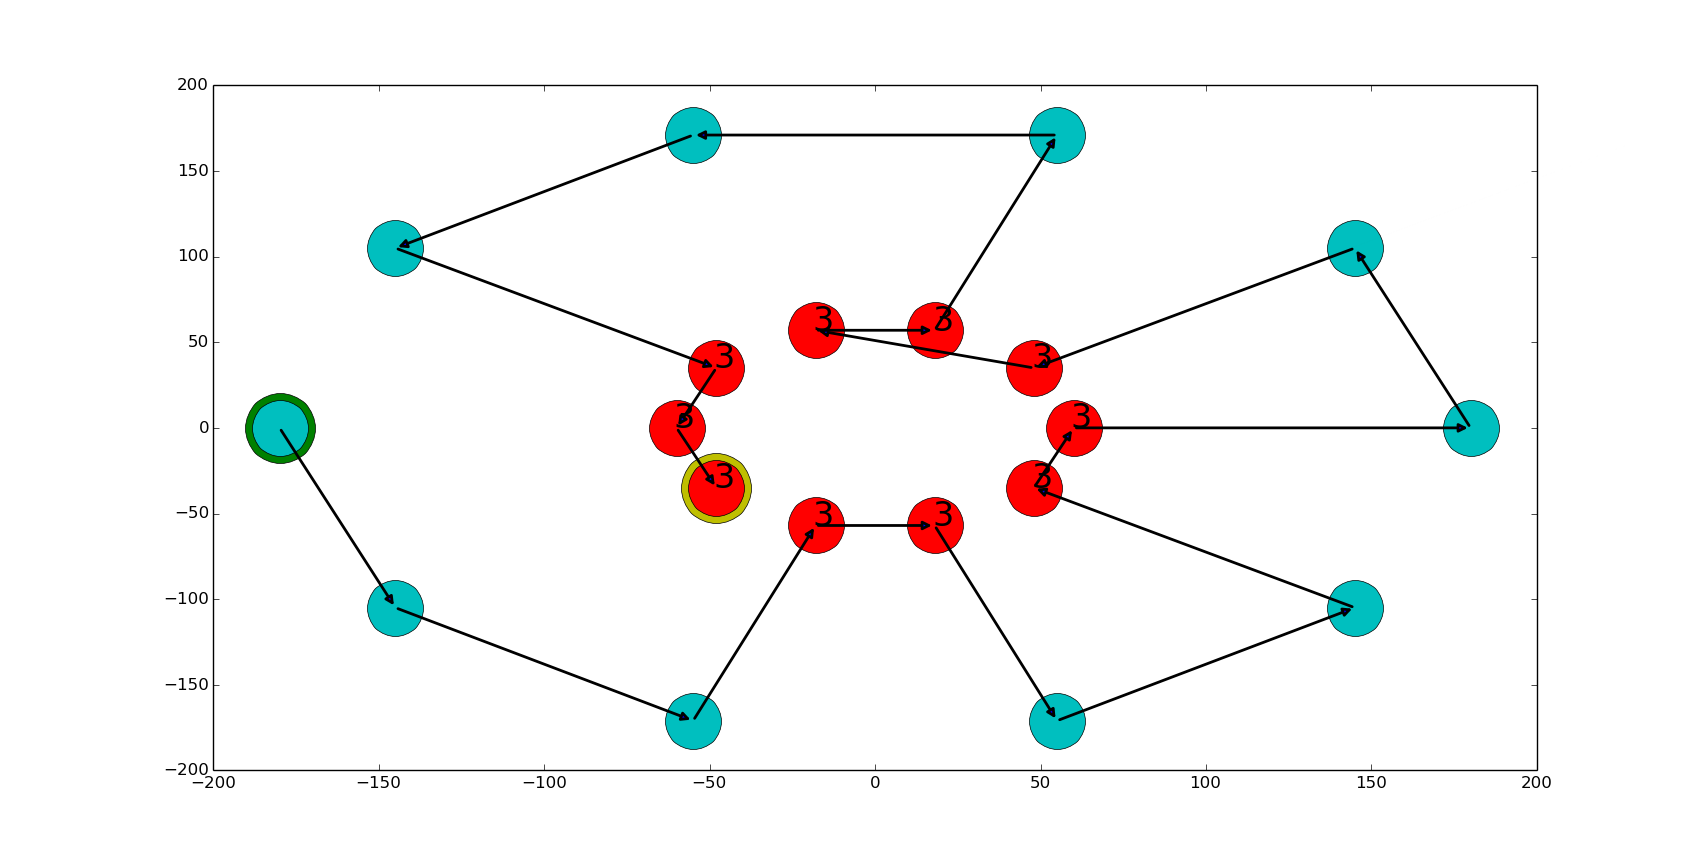
\includegraphics[scale=0.3]{./EJ4/fam72opt.png}\\
 {            \textit{Soluci\'on TABU 2-OPT}}
  \end{center}
  \vspace*{0.3cm}

\vspace*{0.3cm} \vspace*{0.3cm}
  \begin{center}
 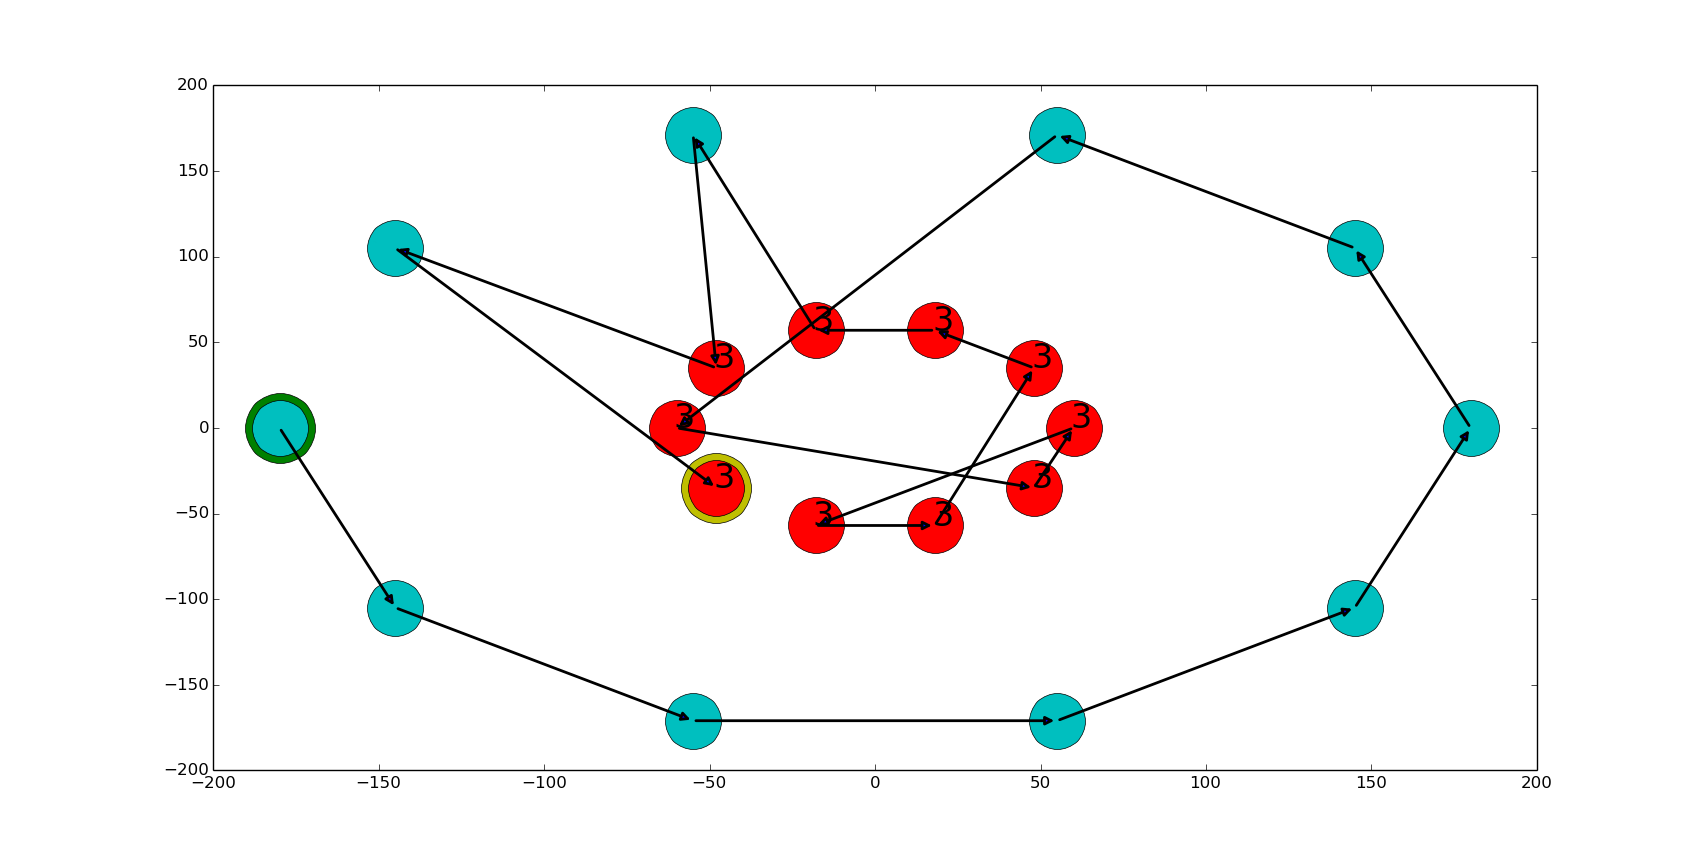
\includegraphics[scale=0.3]{./EJ4/fam73opt.png}\\
 {            \textit{Soluci\'on TABU 3-OPT}}
  \end{center}
  \vspace*{0.3cm}

-----> ACOMODARLO

Veamos como se comporta Tabu 2-OPT con respecto a la heuristica de busqueda local 2-OPT:

\vspace*{0.3cm} \vspace*{0.3cm}
  \begin{center}
 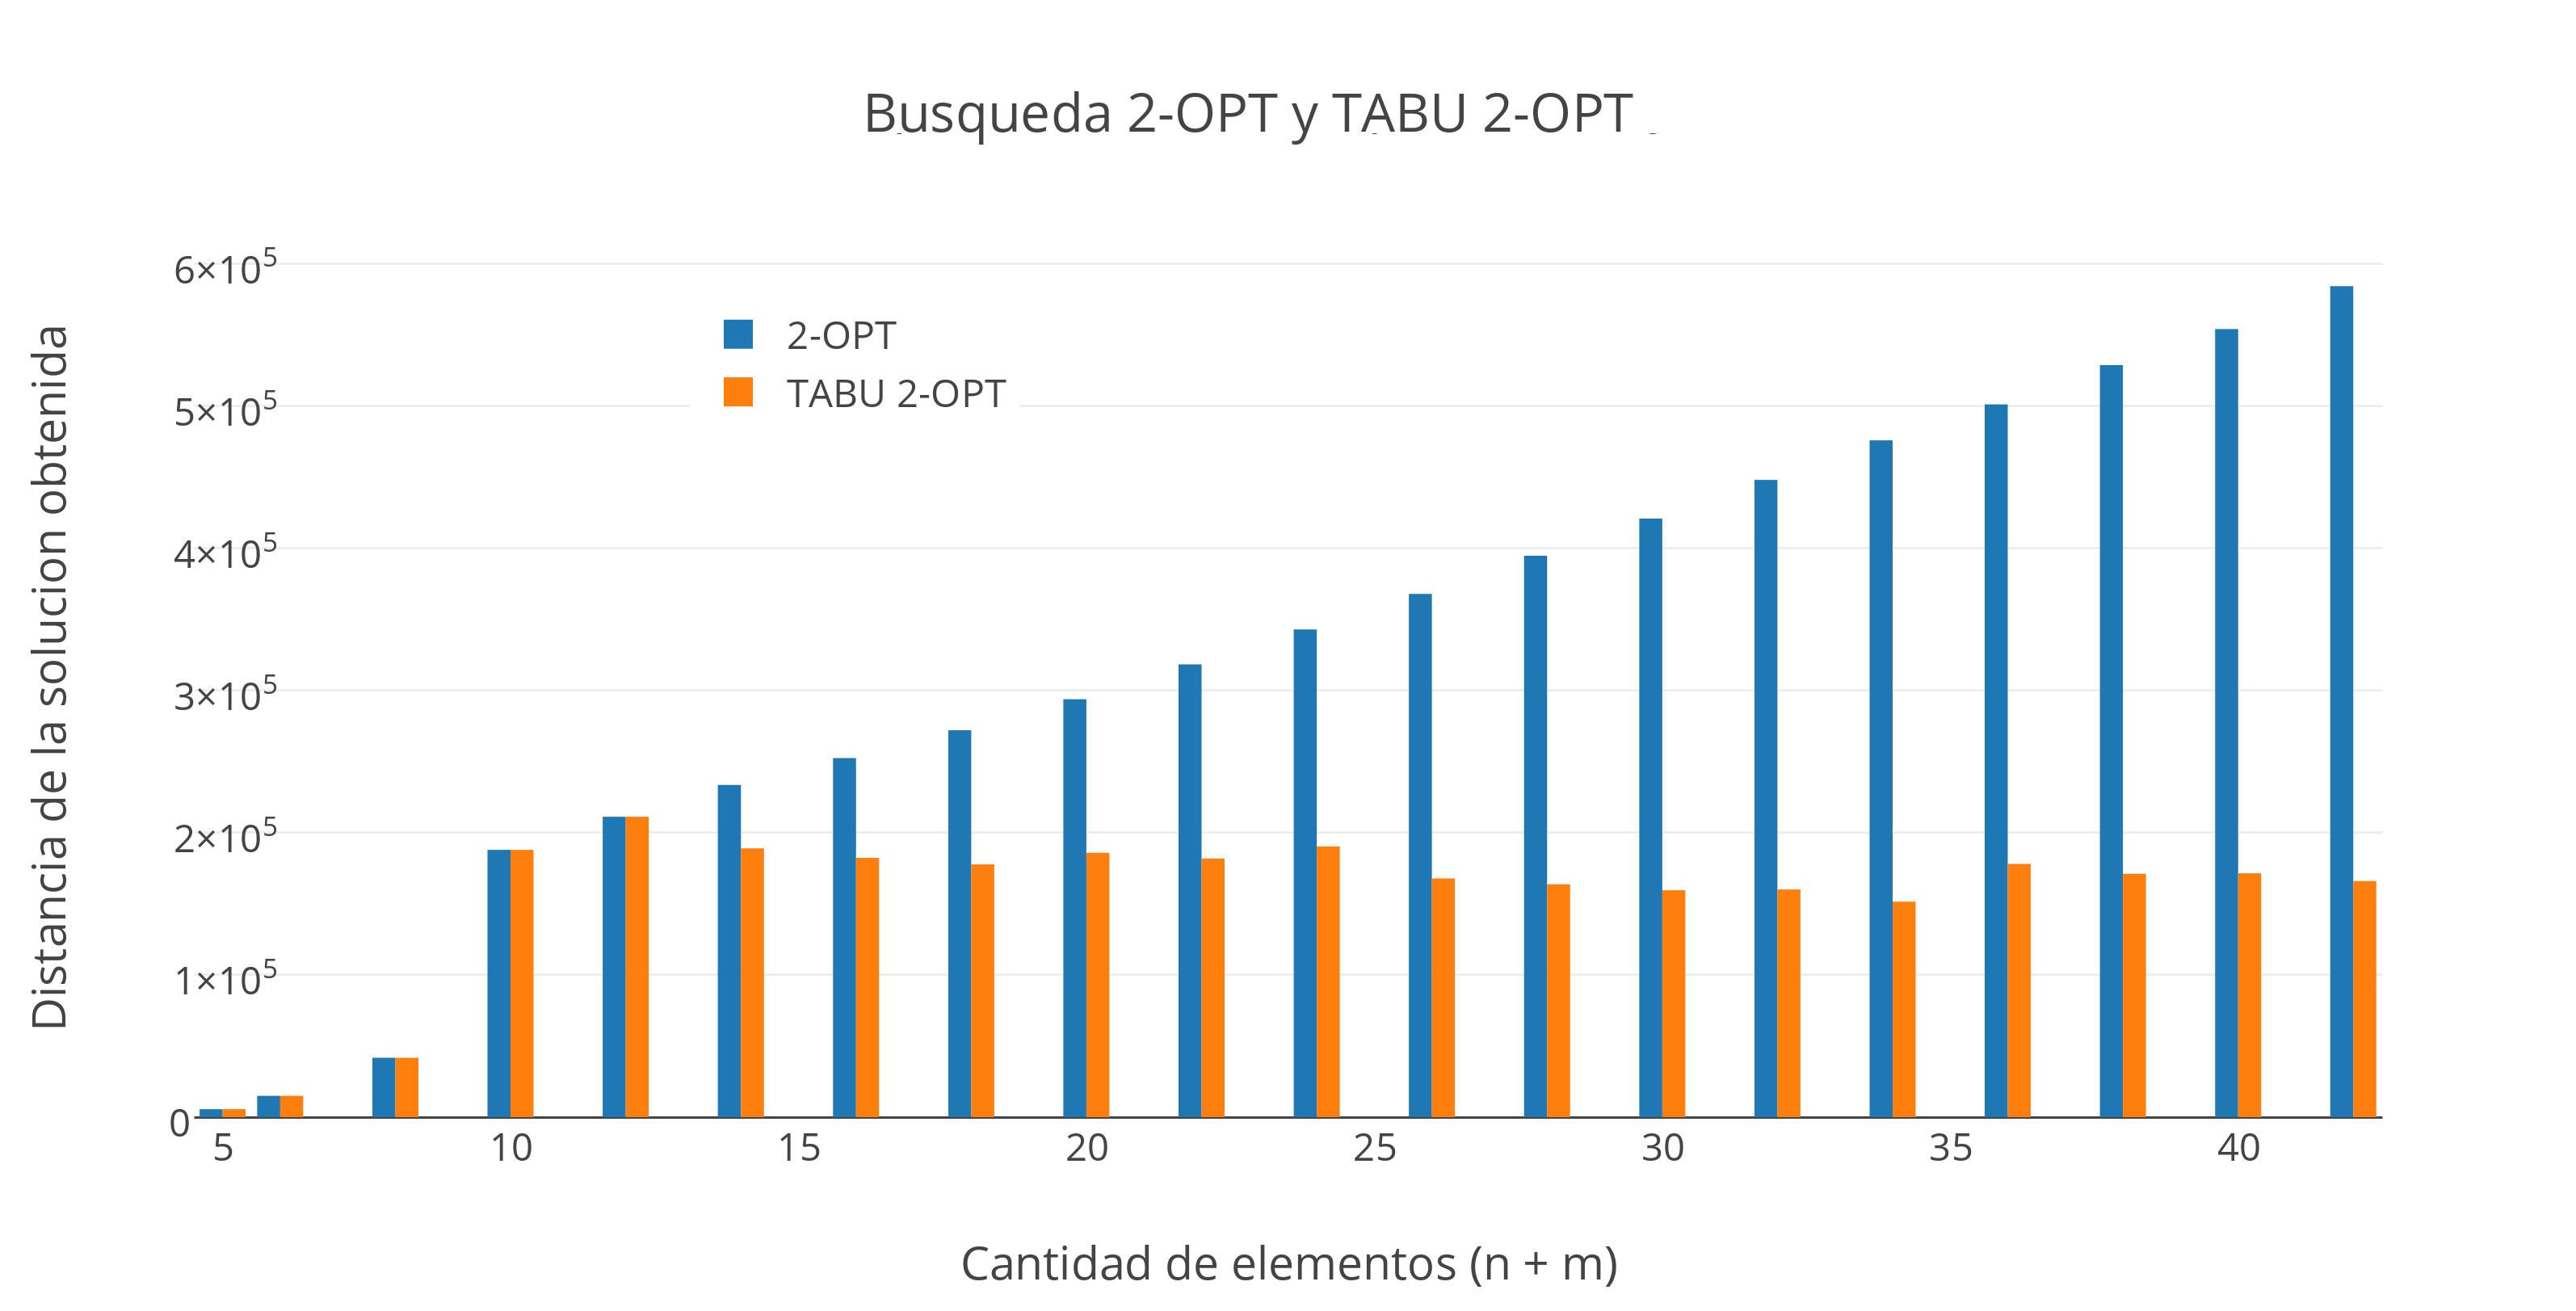
\includegraphics[scale=0.5]{./EJ4/comparativoanillos2opt.png}\\
 {            \textit{Gráfico \ 4.7 - 2-OPT vs Tabu 2-OPT sobre Familia 7}}
  \end{center}
  \vspace*{0.3cm}

En cuanto a tiempo insumido vemos lo siguiente:

\vspace*{0.3cm} \vspace*{0.3cm}
  \begin{center}
 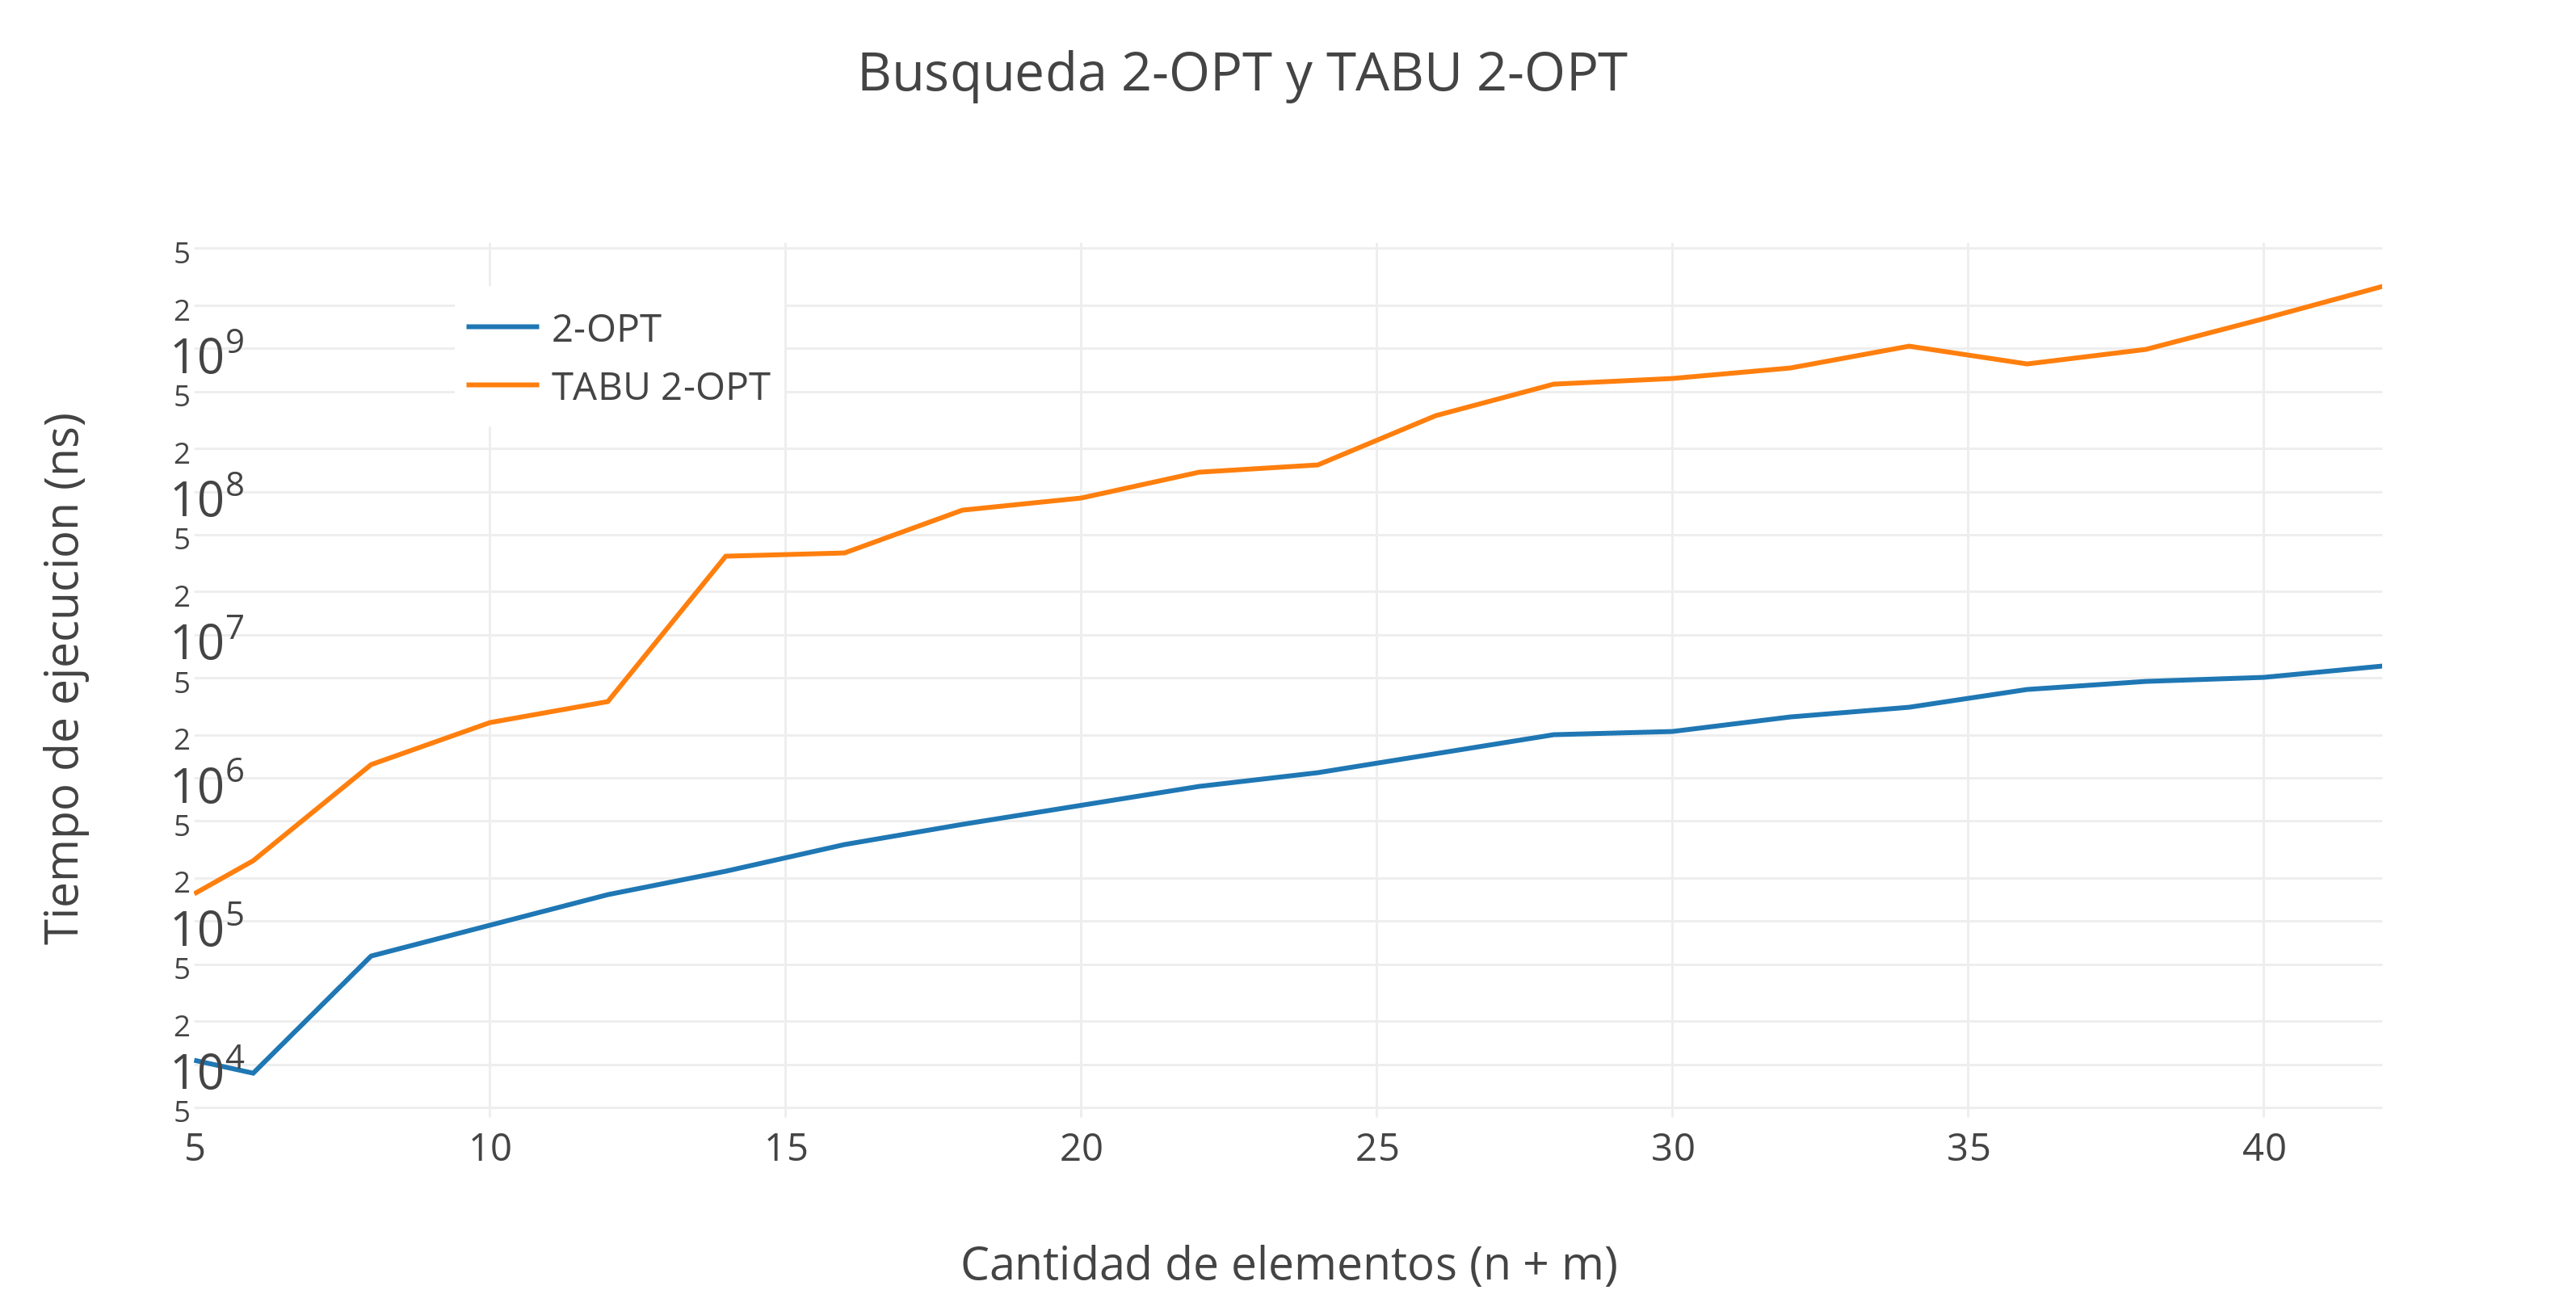
\includegraphics[scale=0.5]{./EJ4/medicionanillos2opt.png}\\
 {            \textit{Gráfico \ 4.8 - 2-OPT vs Tabu 2-OPT sobre Familia 7}}
  \end{center}
  \vspace*{0.3cm}


Luego, para 3-OPT:

\vspace*{0.3cm} \vspace*{0.3cm}
  \begin{center}
 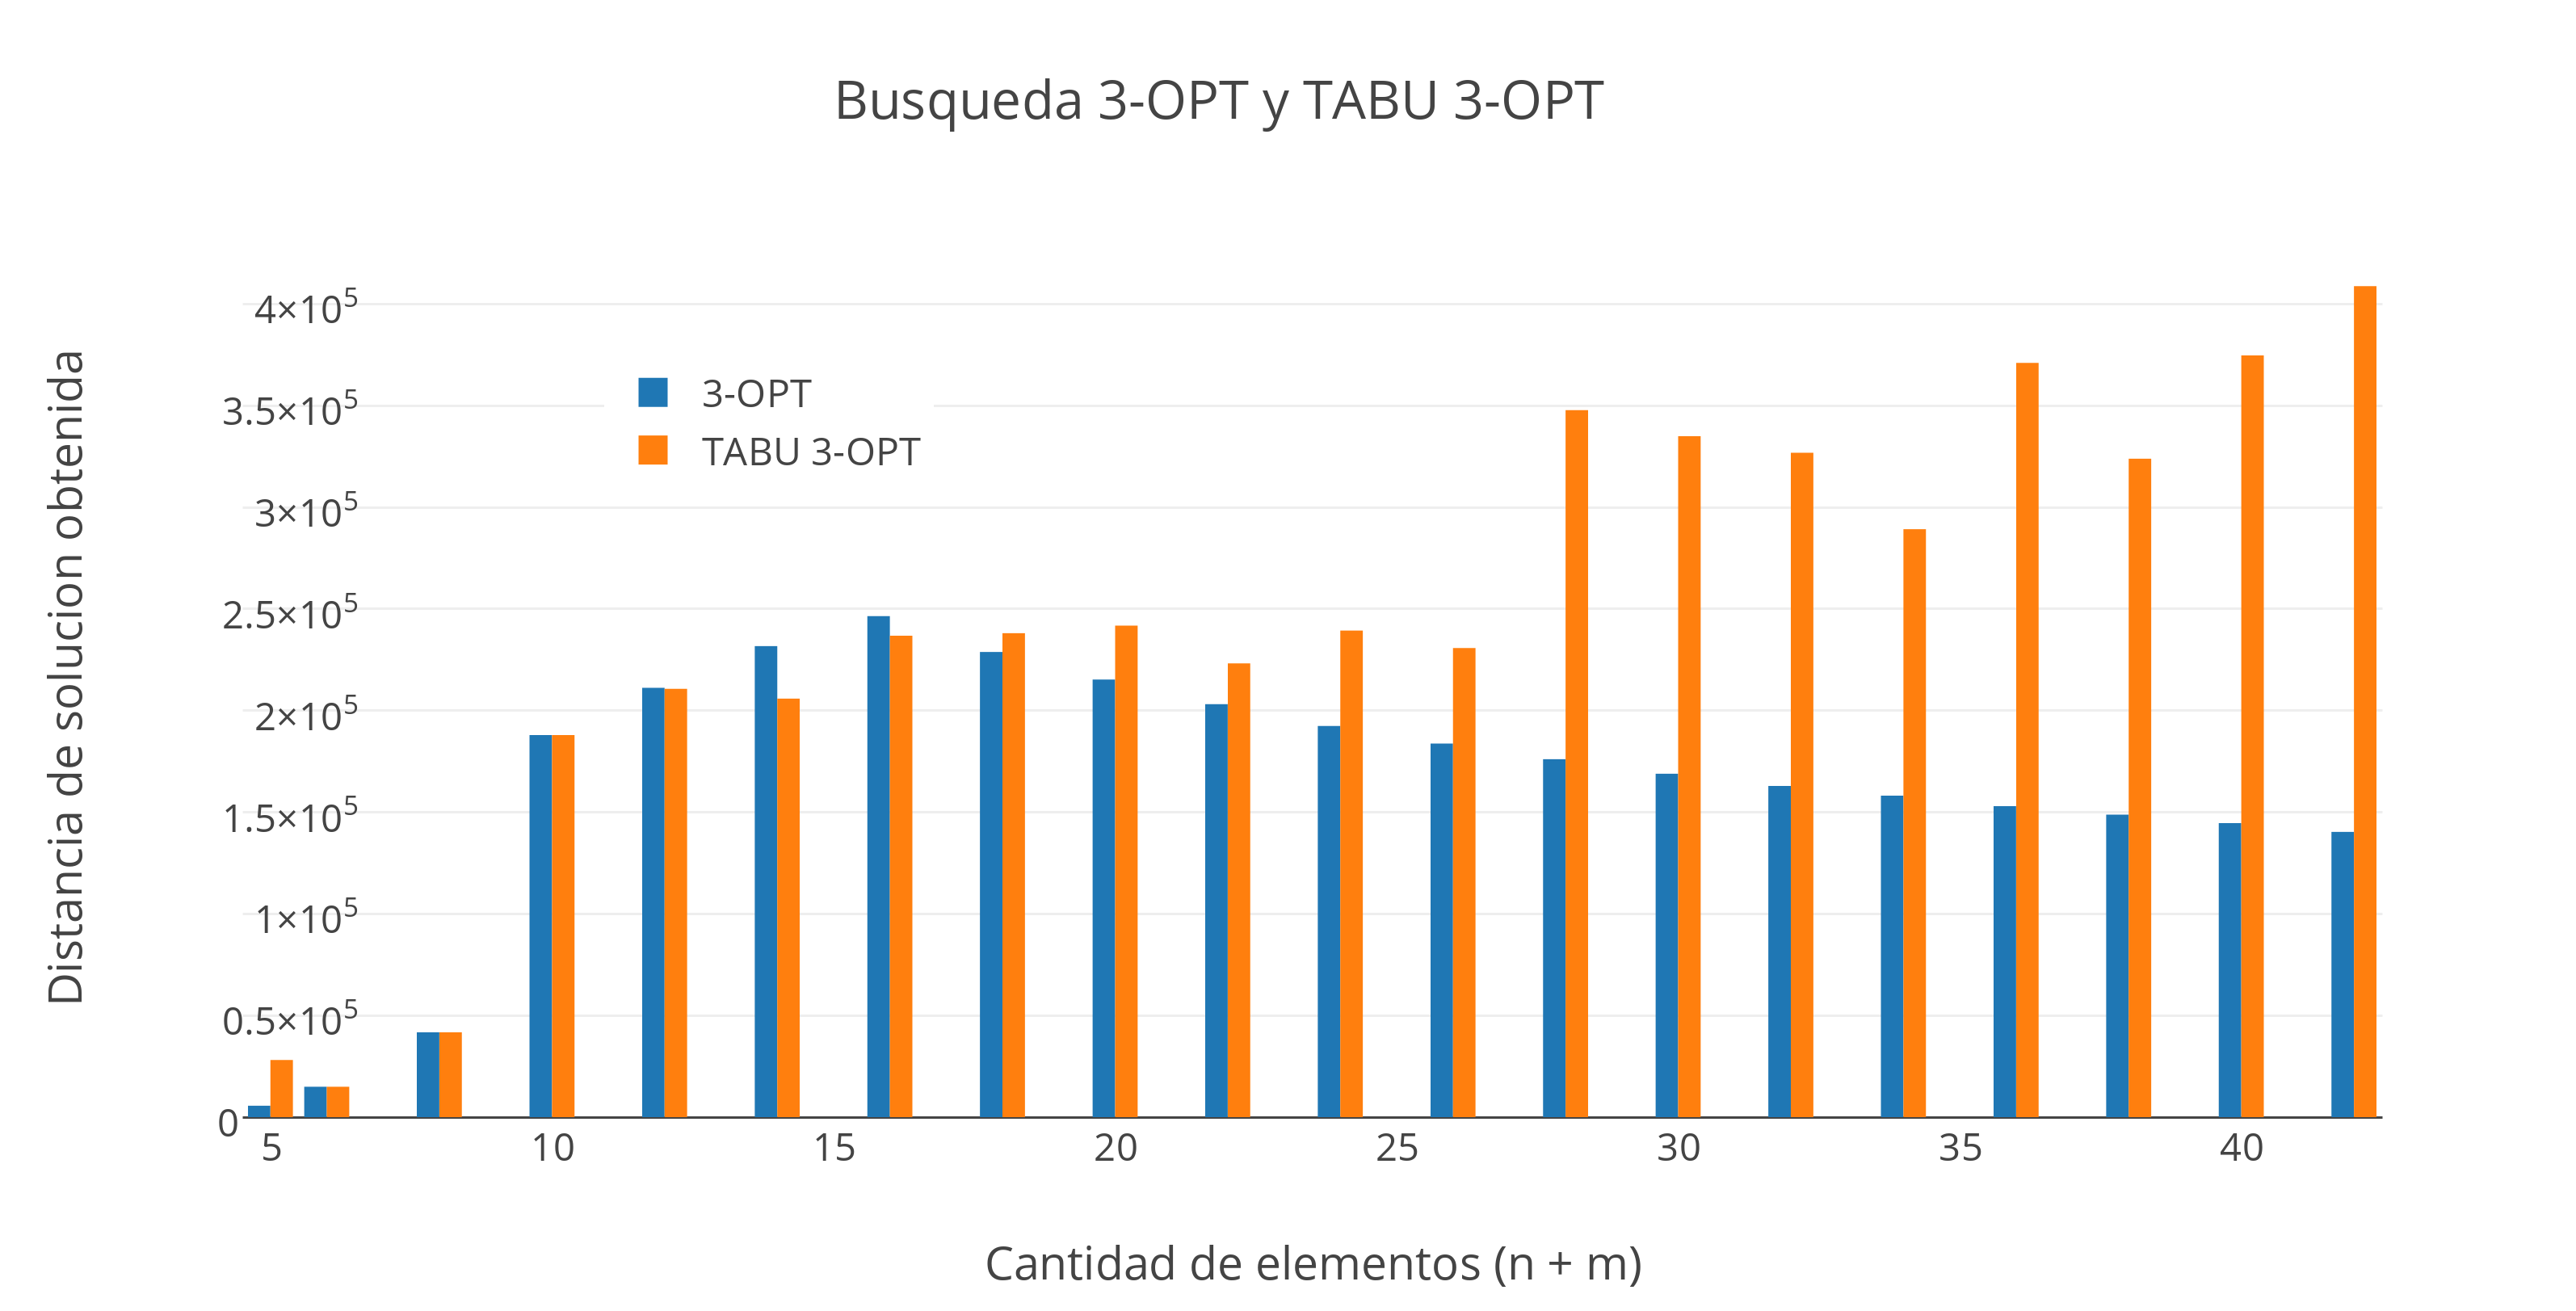
\includegraphics[scale=0.5]{./EJ4/comparativoanillos3opt.png}\\
 {            \textit{Gráfico \ 4.9 - 3-OPT vs Tabu 3-OPT sobre Familia 7}}
  \end{center}
  \vspace*{0.3cm}

En cuanto a tiempo insumido vemos lo siguiente:

\vspace*{0.3cm} \vspace*{0.3cm}
  \begin{center}
 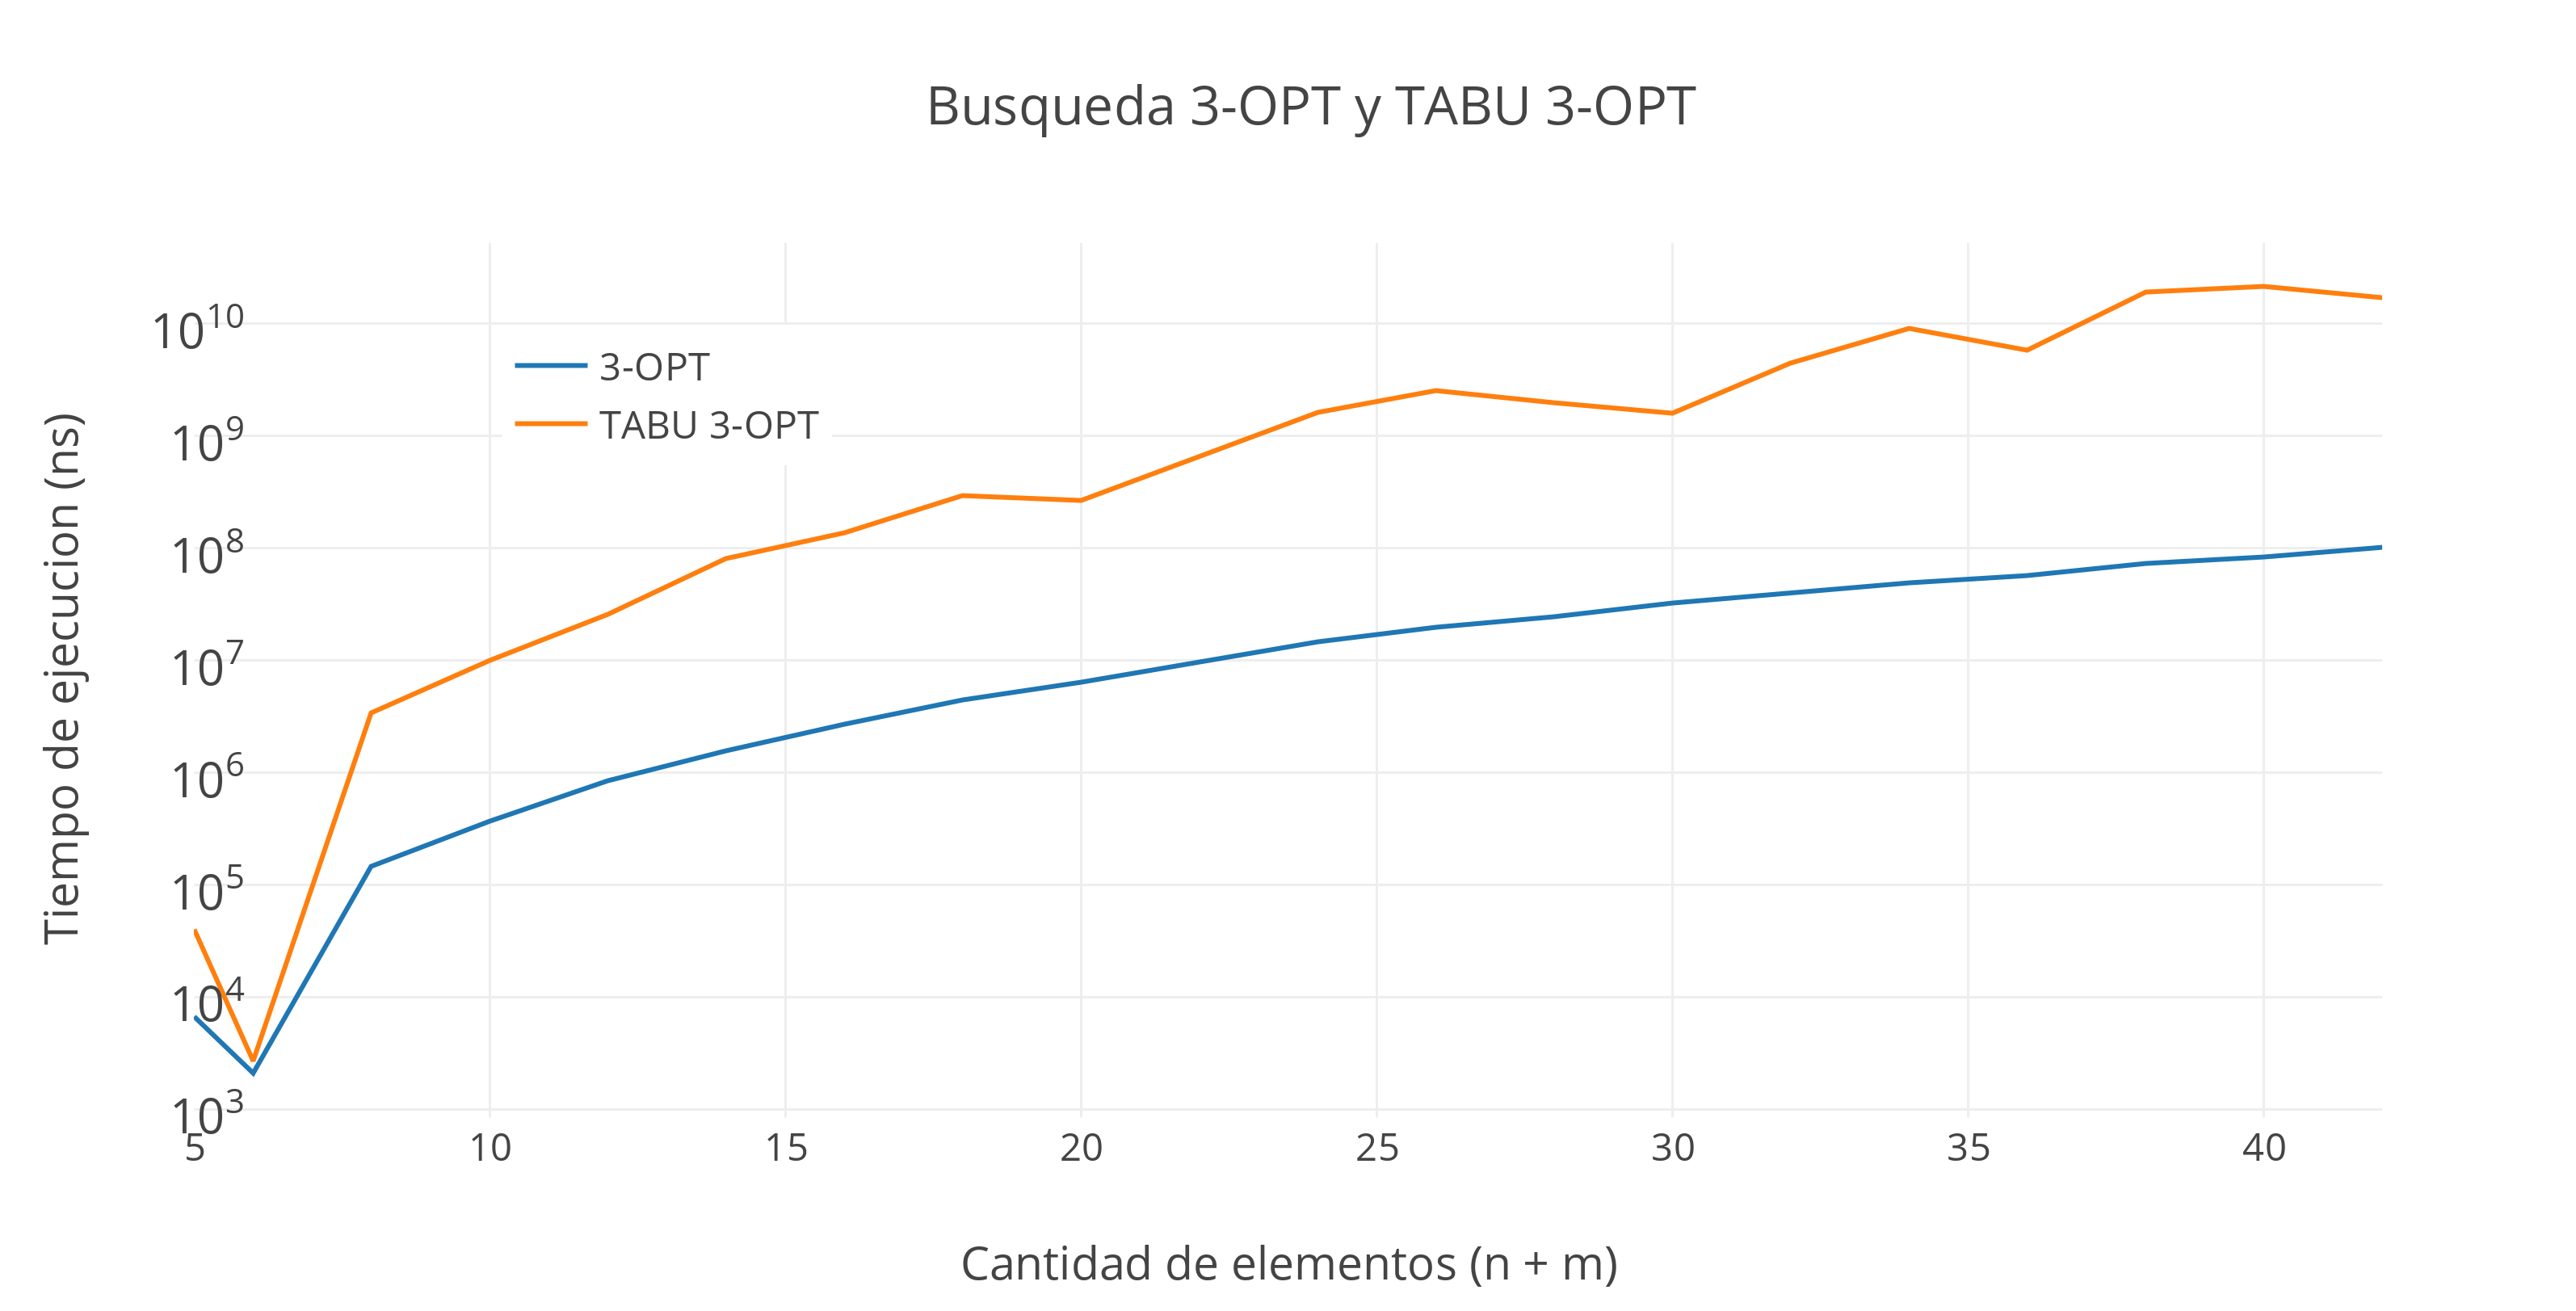
\includegraphics[scale=0.5]{./EJ4/medicionanillos3opt.png}\\
 {            \textit{Gráfico \ 4.10 - 3-OPT vs Tabu 3-OPT sobre Familia 7}}
  \end{center}
  \vspace*{0.3cm}
  
Para la comparación entre algoritmos tabu, se comparará conjuntamente el tiempo de ejecución con la calidad de la solución. Para esta última tendremos en cuenta que los algoritmos, de devolver un resultado, será válido: esto quiere decir que cuanto menor distancia recorran en las soluciones, mejor serán las mismas:

Las soluciones obtenidas fueron las siguientes:

\vspace*{0.3cm} \vspace*{0.3cm}
  \begin{center}
 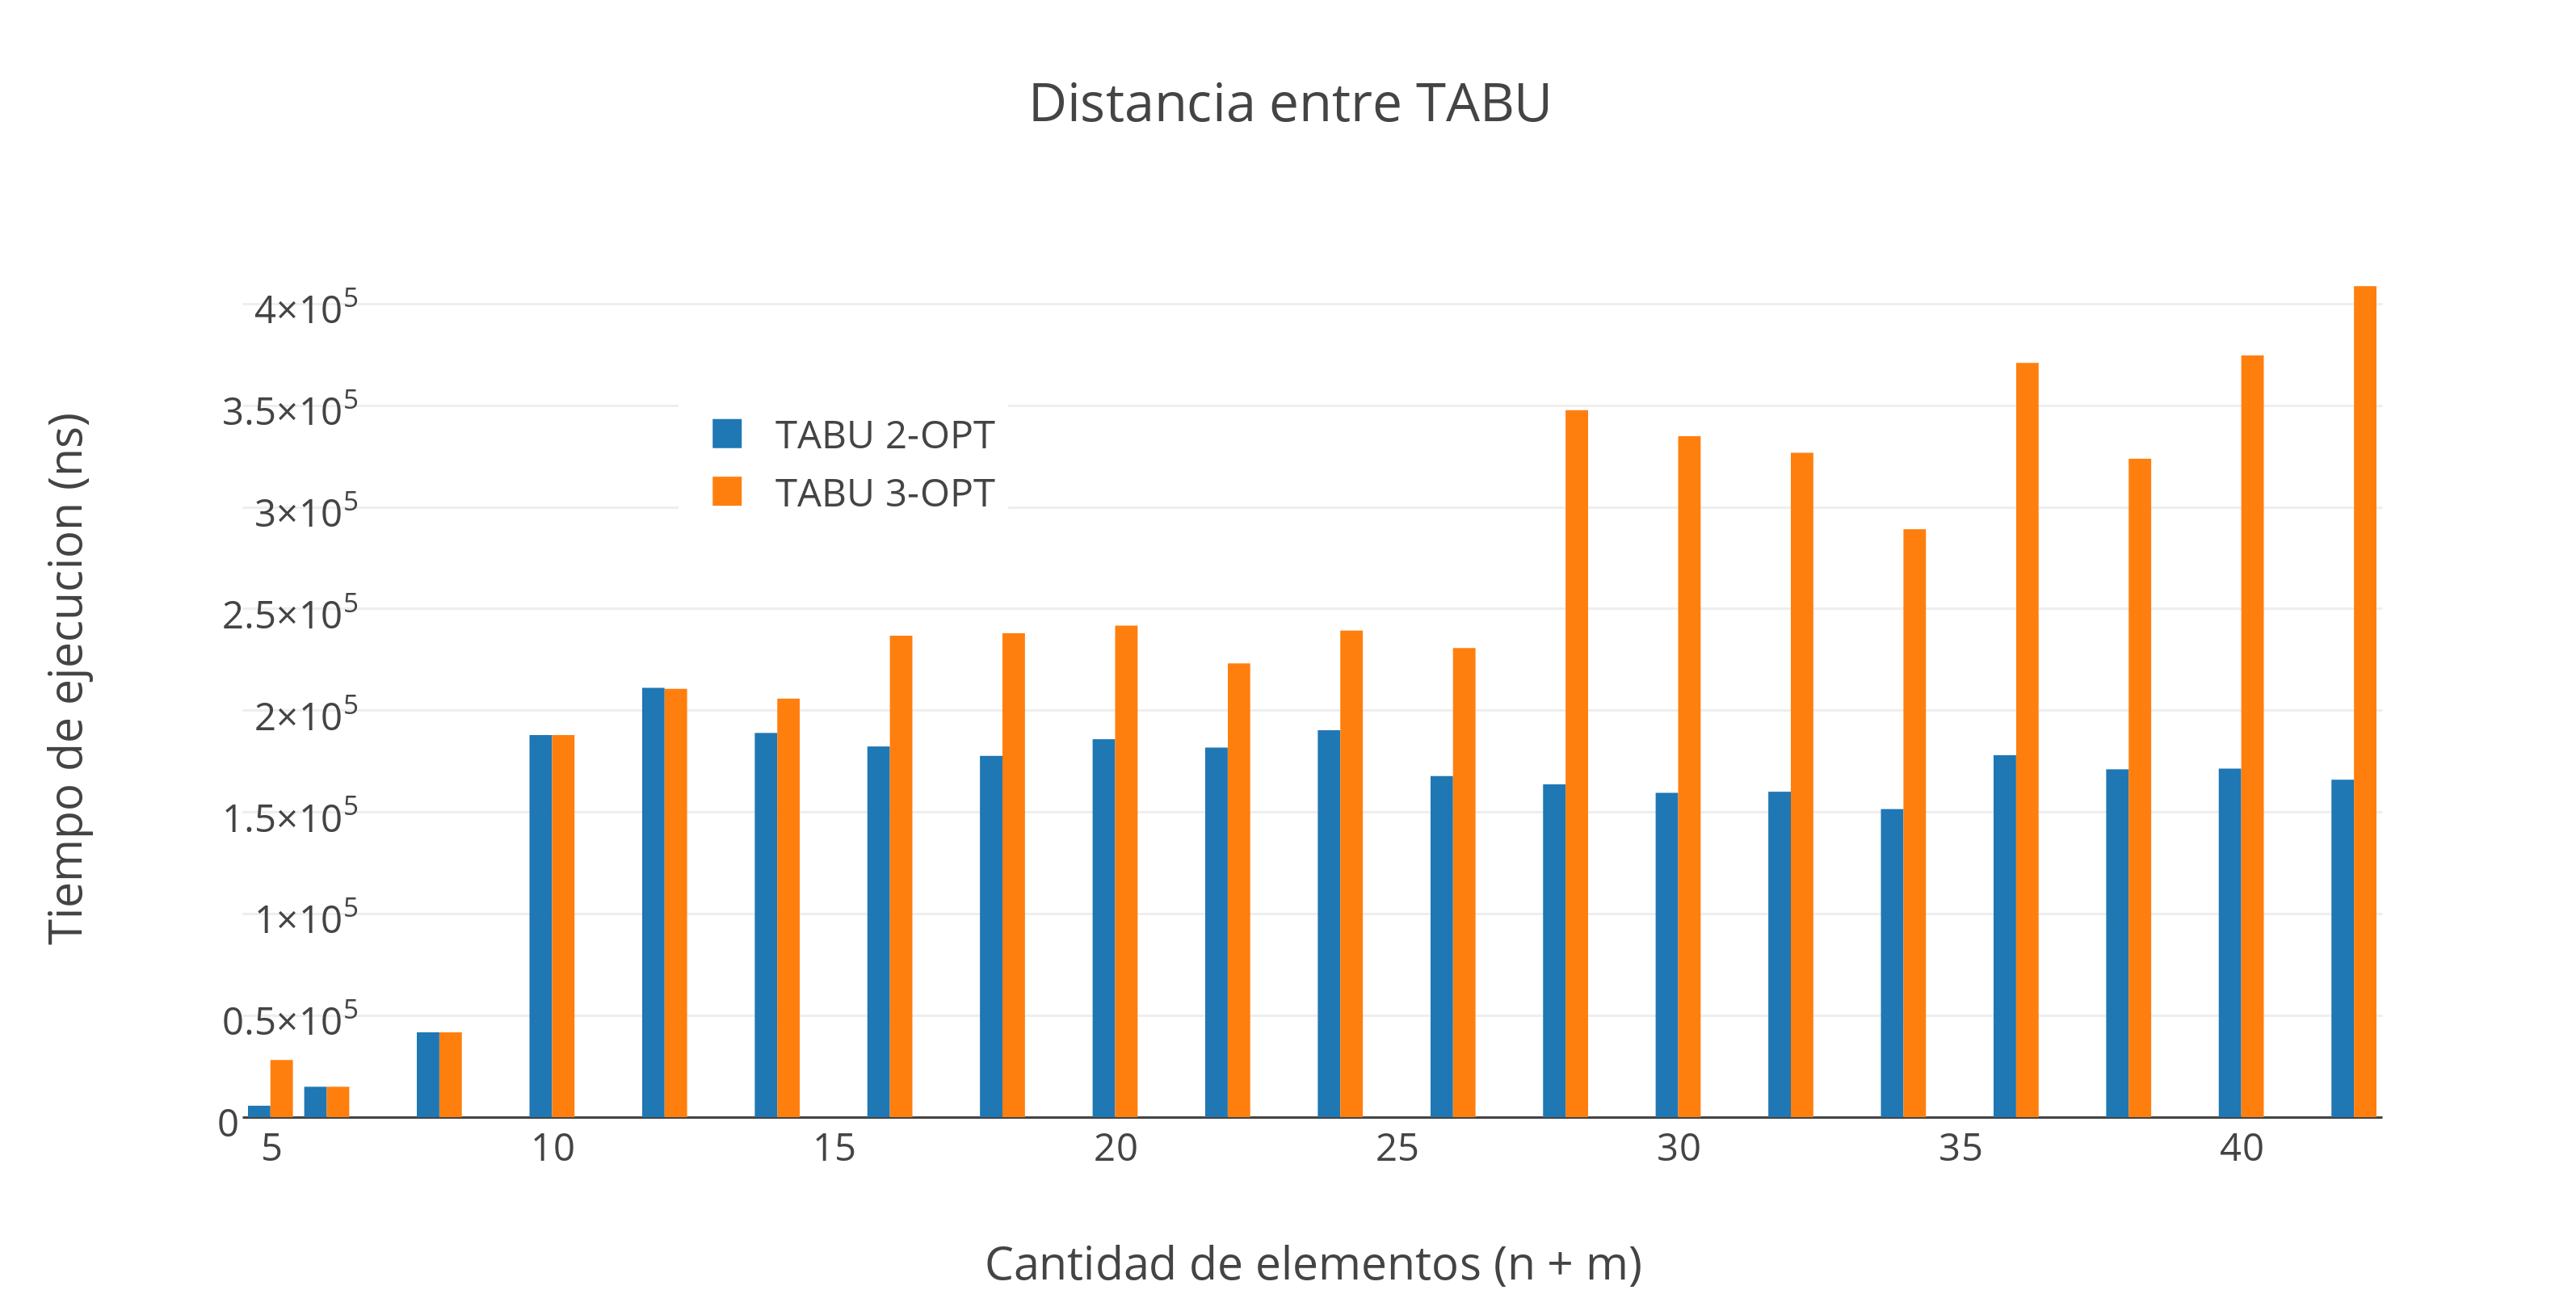
\includegraphics[scale=0.5]{./EJ4/comparativoanillos1.png}\\
 {            \textit{Gráfico \ 4.11 - Tabu 2-OPT vs Tabu 3-OPT sobre Familia 7}}
  \end{center}
  \vspace*{0.3cm}

En cuanto a tiempo insumido vemos lo siguiente:

\vspace*{0.3cm} \vspace*{0.3cm}
  \begin{center}
 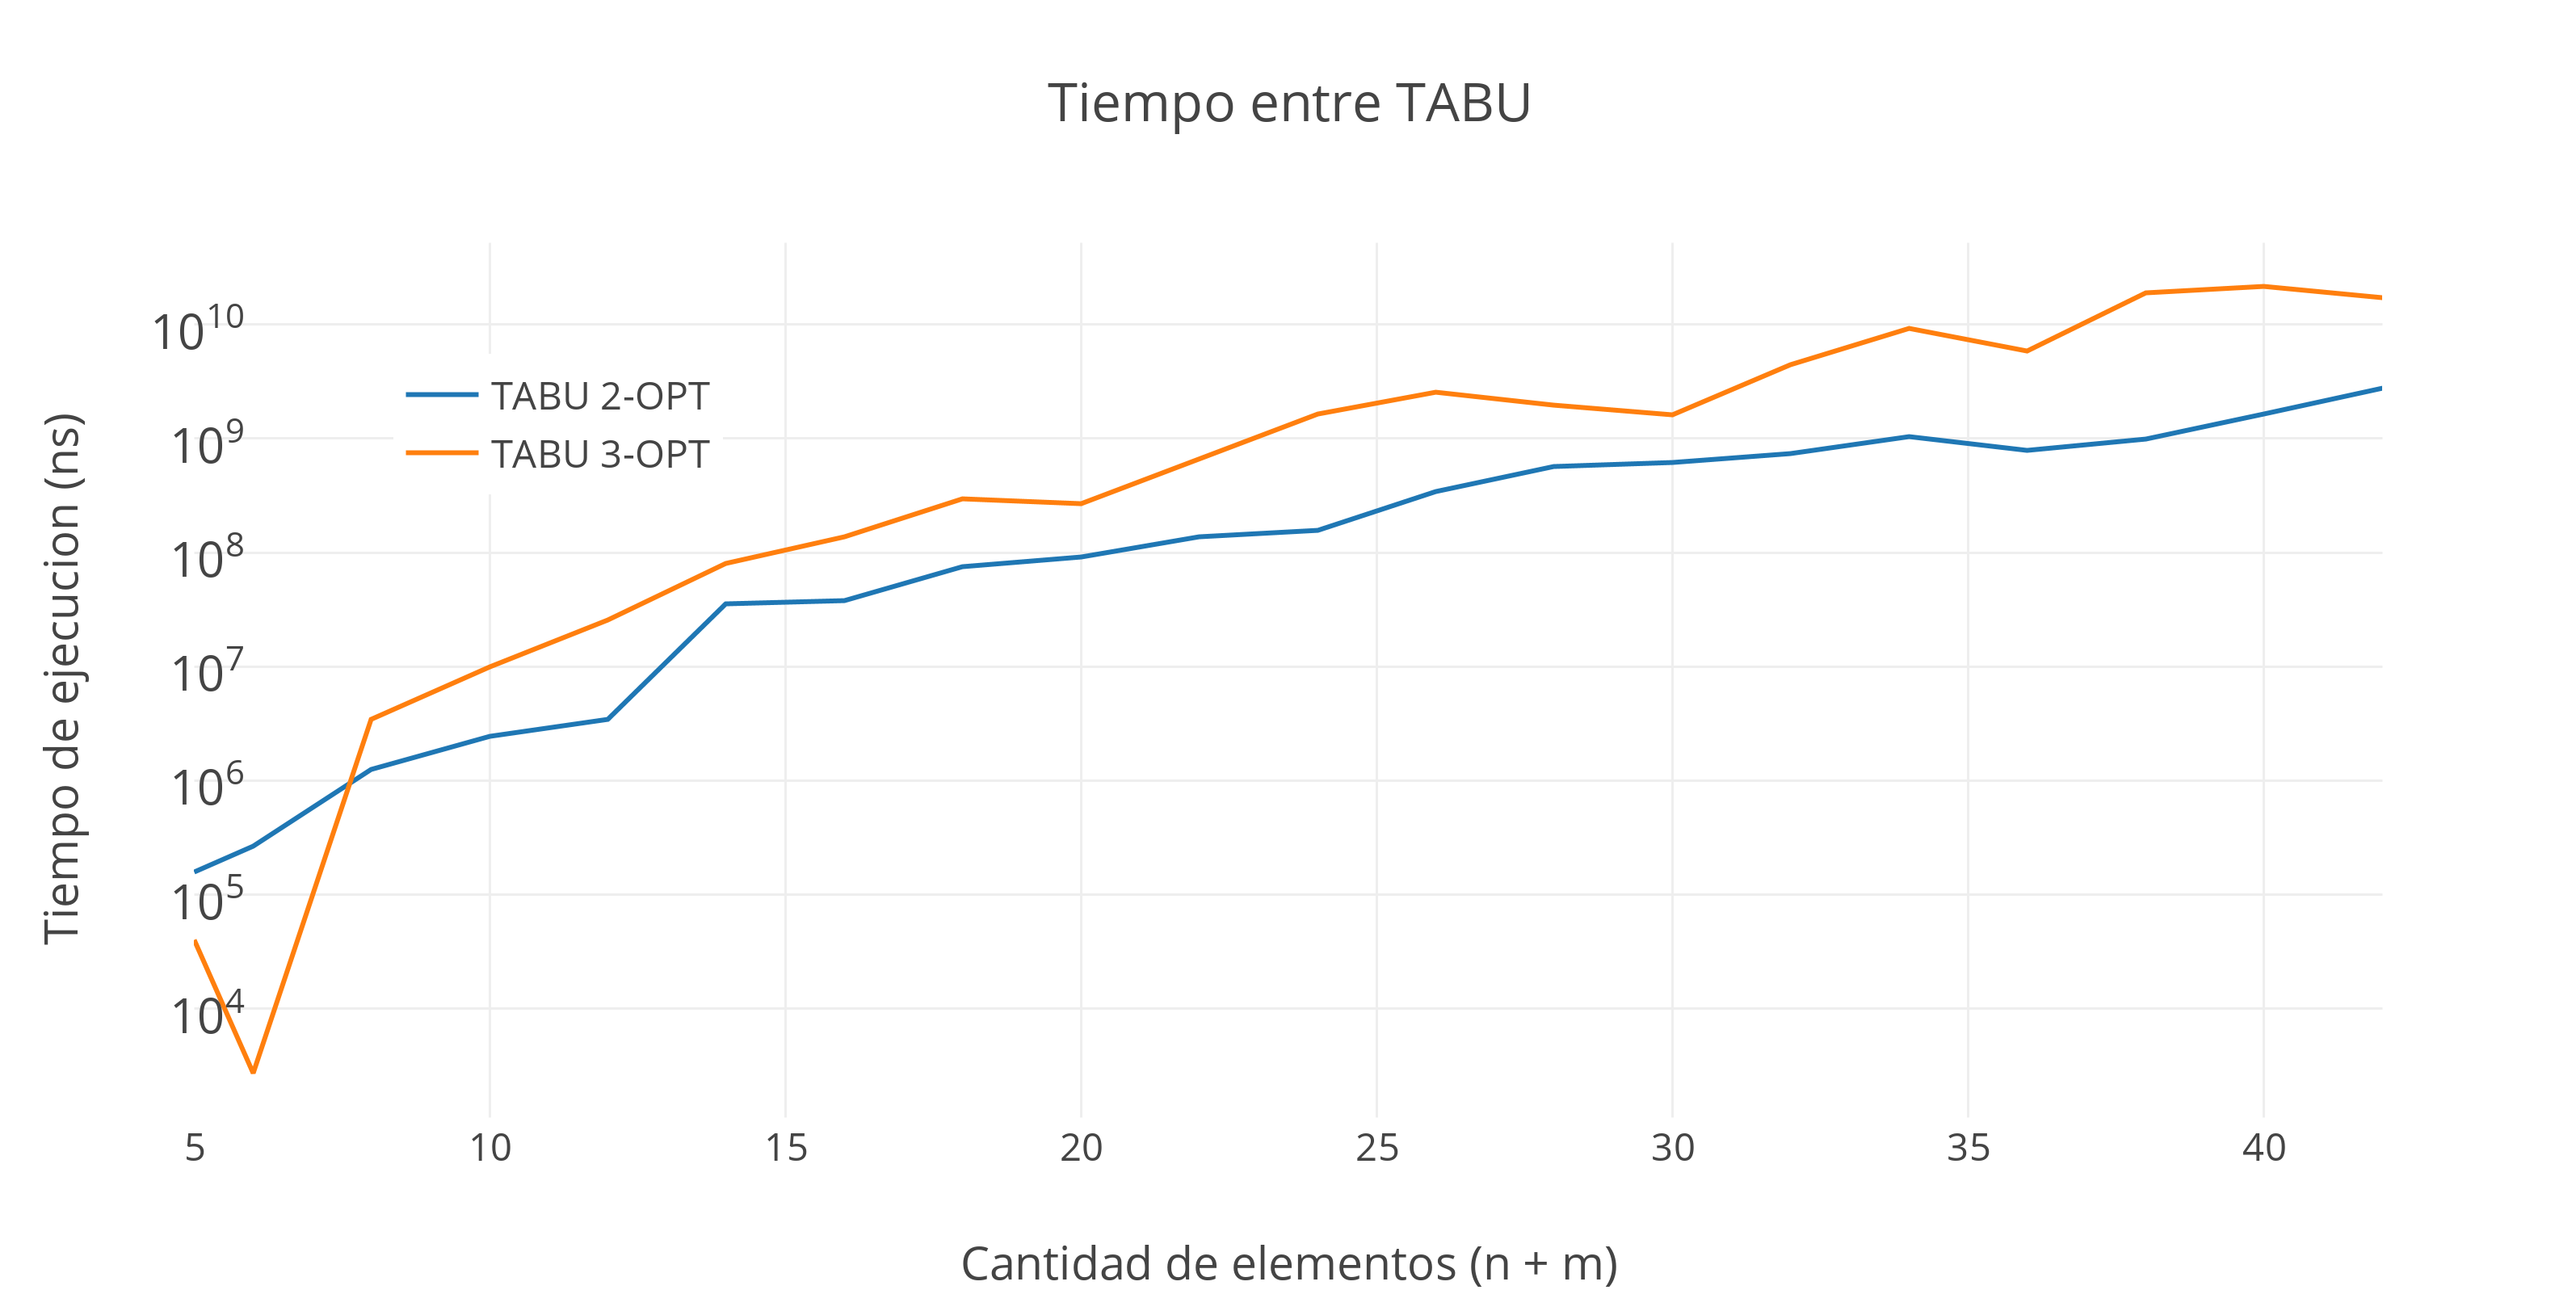
\includegraphics[scale=0.5]{./EJ4/comparativoanillos.png}\\
 {            \textit{Gráfico \ 4.12 - Tabu 2-OPT vs Tabu 3-OPT sobre Familia 7}}
  \end{center}
  \vspace*{0.3cm}

  
  
\subsubsection*{Familia 8}

\vspace*{0.3cm} \vspace*{0.3cm}
  \begin{center}
 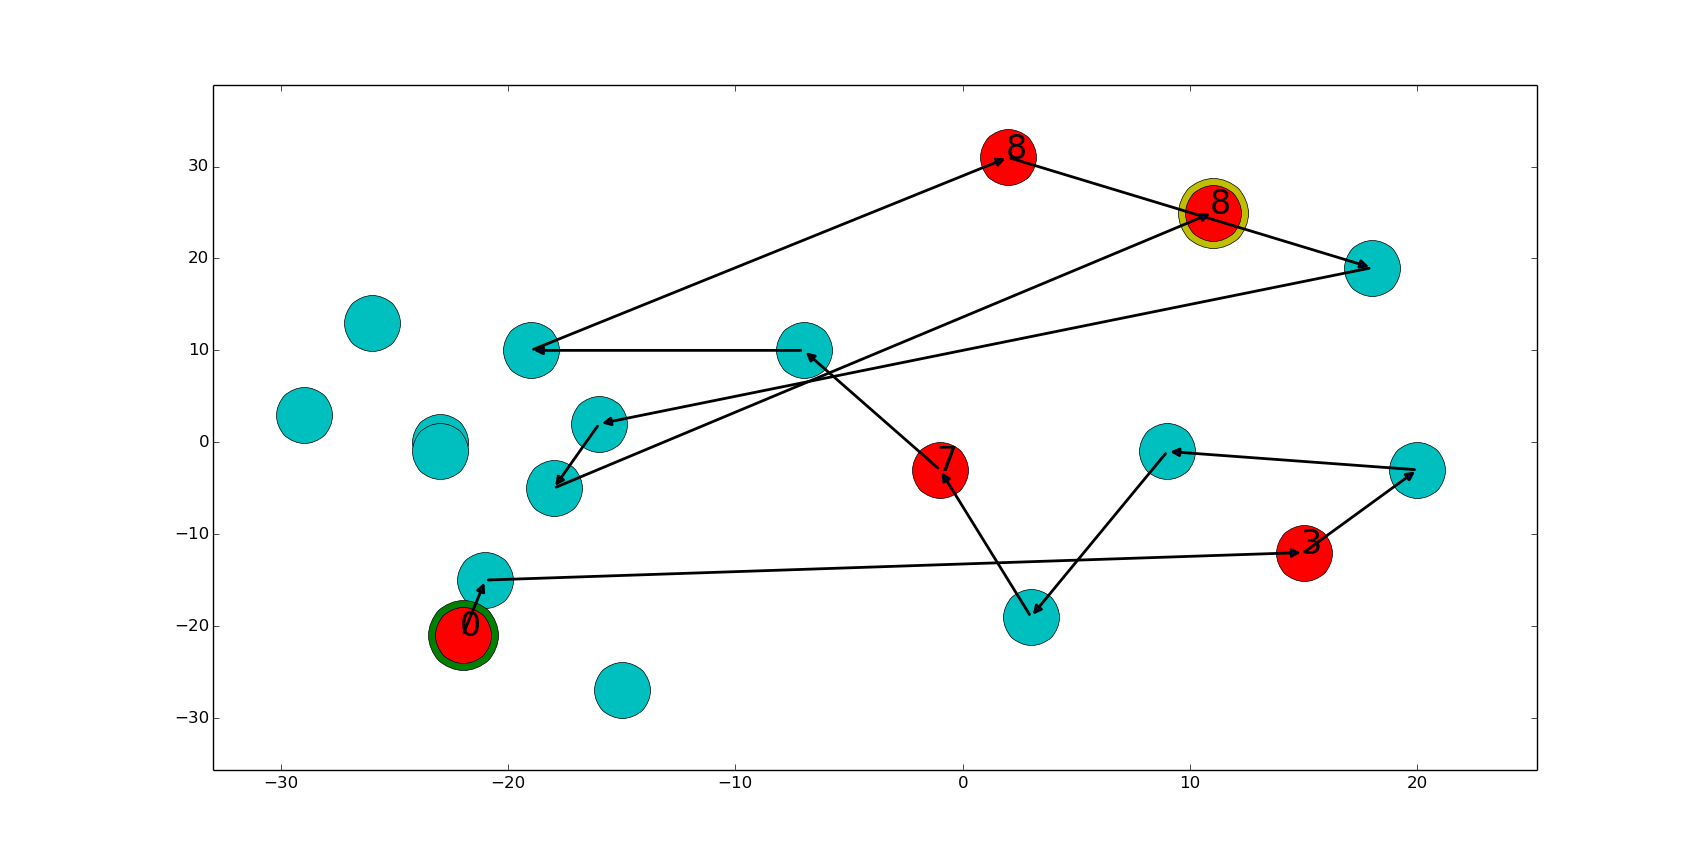
\includegraphics[scale=0.3]{./EJ4/fam8goloso.png}\\
 {            \textit{Soluci\'on Golosa}}
  \end{center}
  \vspace*{0.3cm}

\vspace*{0.3cm} \vspace*{0.3cm}
  \begin{center}
 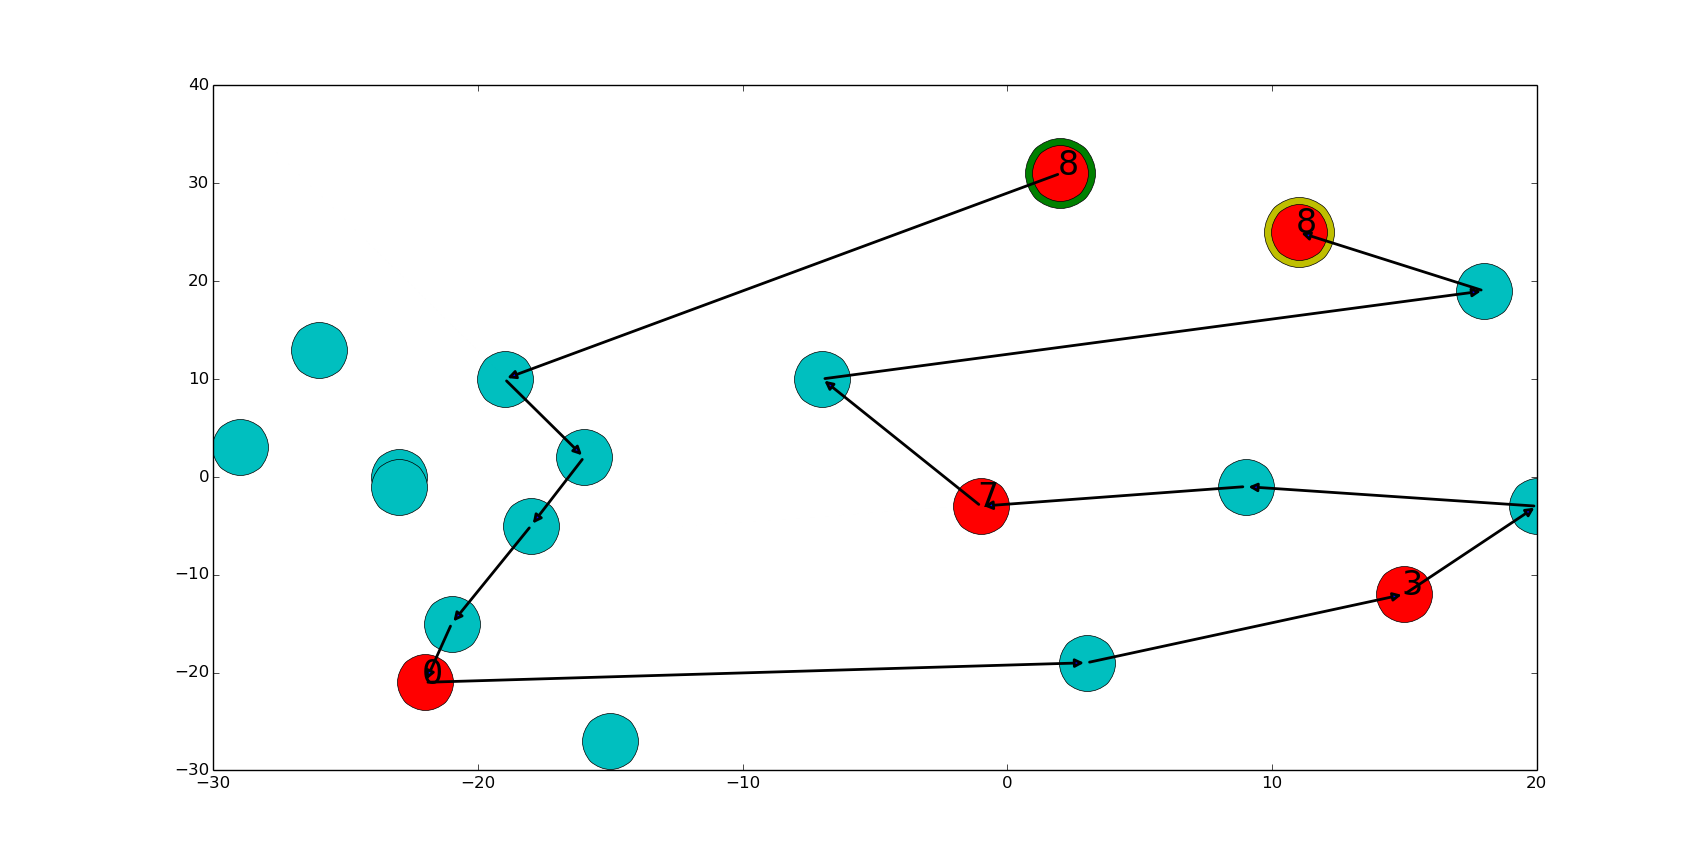
\includegraphics[scale=0.3]{./EJ4/fam82opt.png}\\
 {            \textit{Soluci\'on TABU 2-OPT}}
  \end{center}
  \vspace*{0.3cm}

\vspace*{0.3cm} \vspace*{0.3cm}
  \begin{center}
 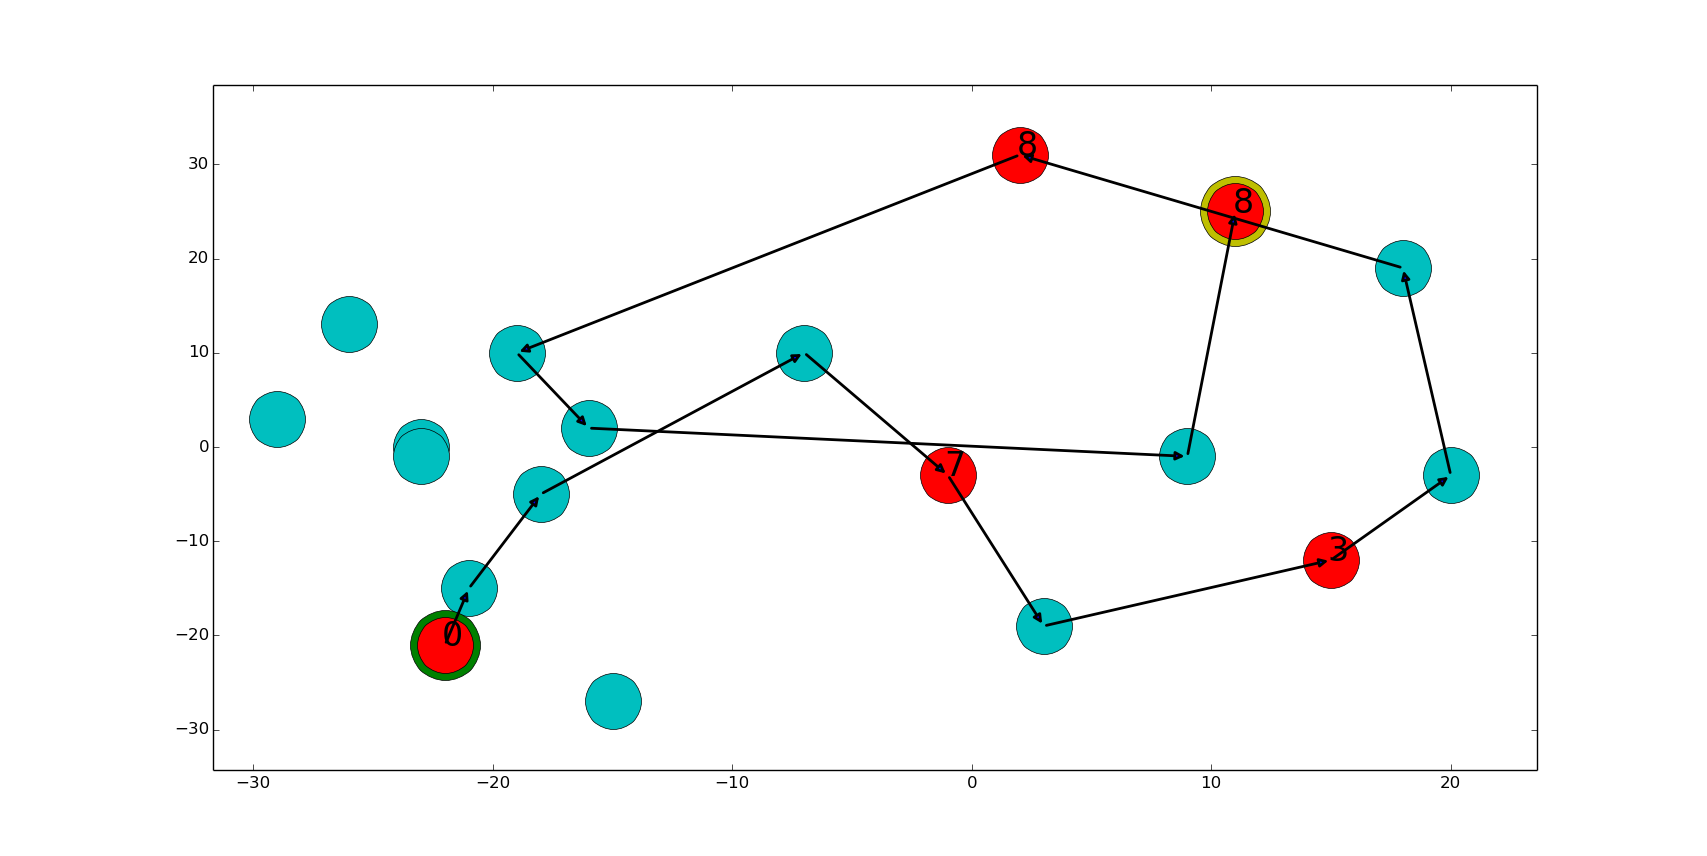
\includegraphics[scale=0.3]{./EJ4/fam83opt.png}\\
 {            \textit{Soluci\'on TABU 3-OPT}}
  \end{center}
  \vspace*{0.3cm}

-----> ACOMODARLO
Veamos como se comporta Tabu 2-OPT con respecto a la heuristica de busqueda local 2-OPT:

\vspace*{0.3cm} \vspace*{0.3cm}
  \begin{center}
 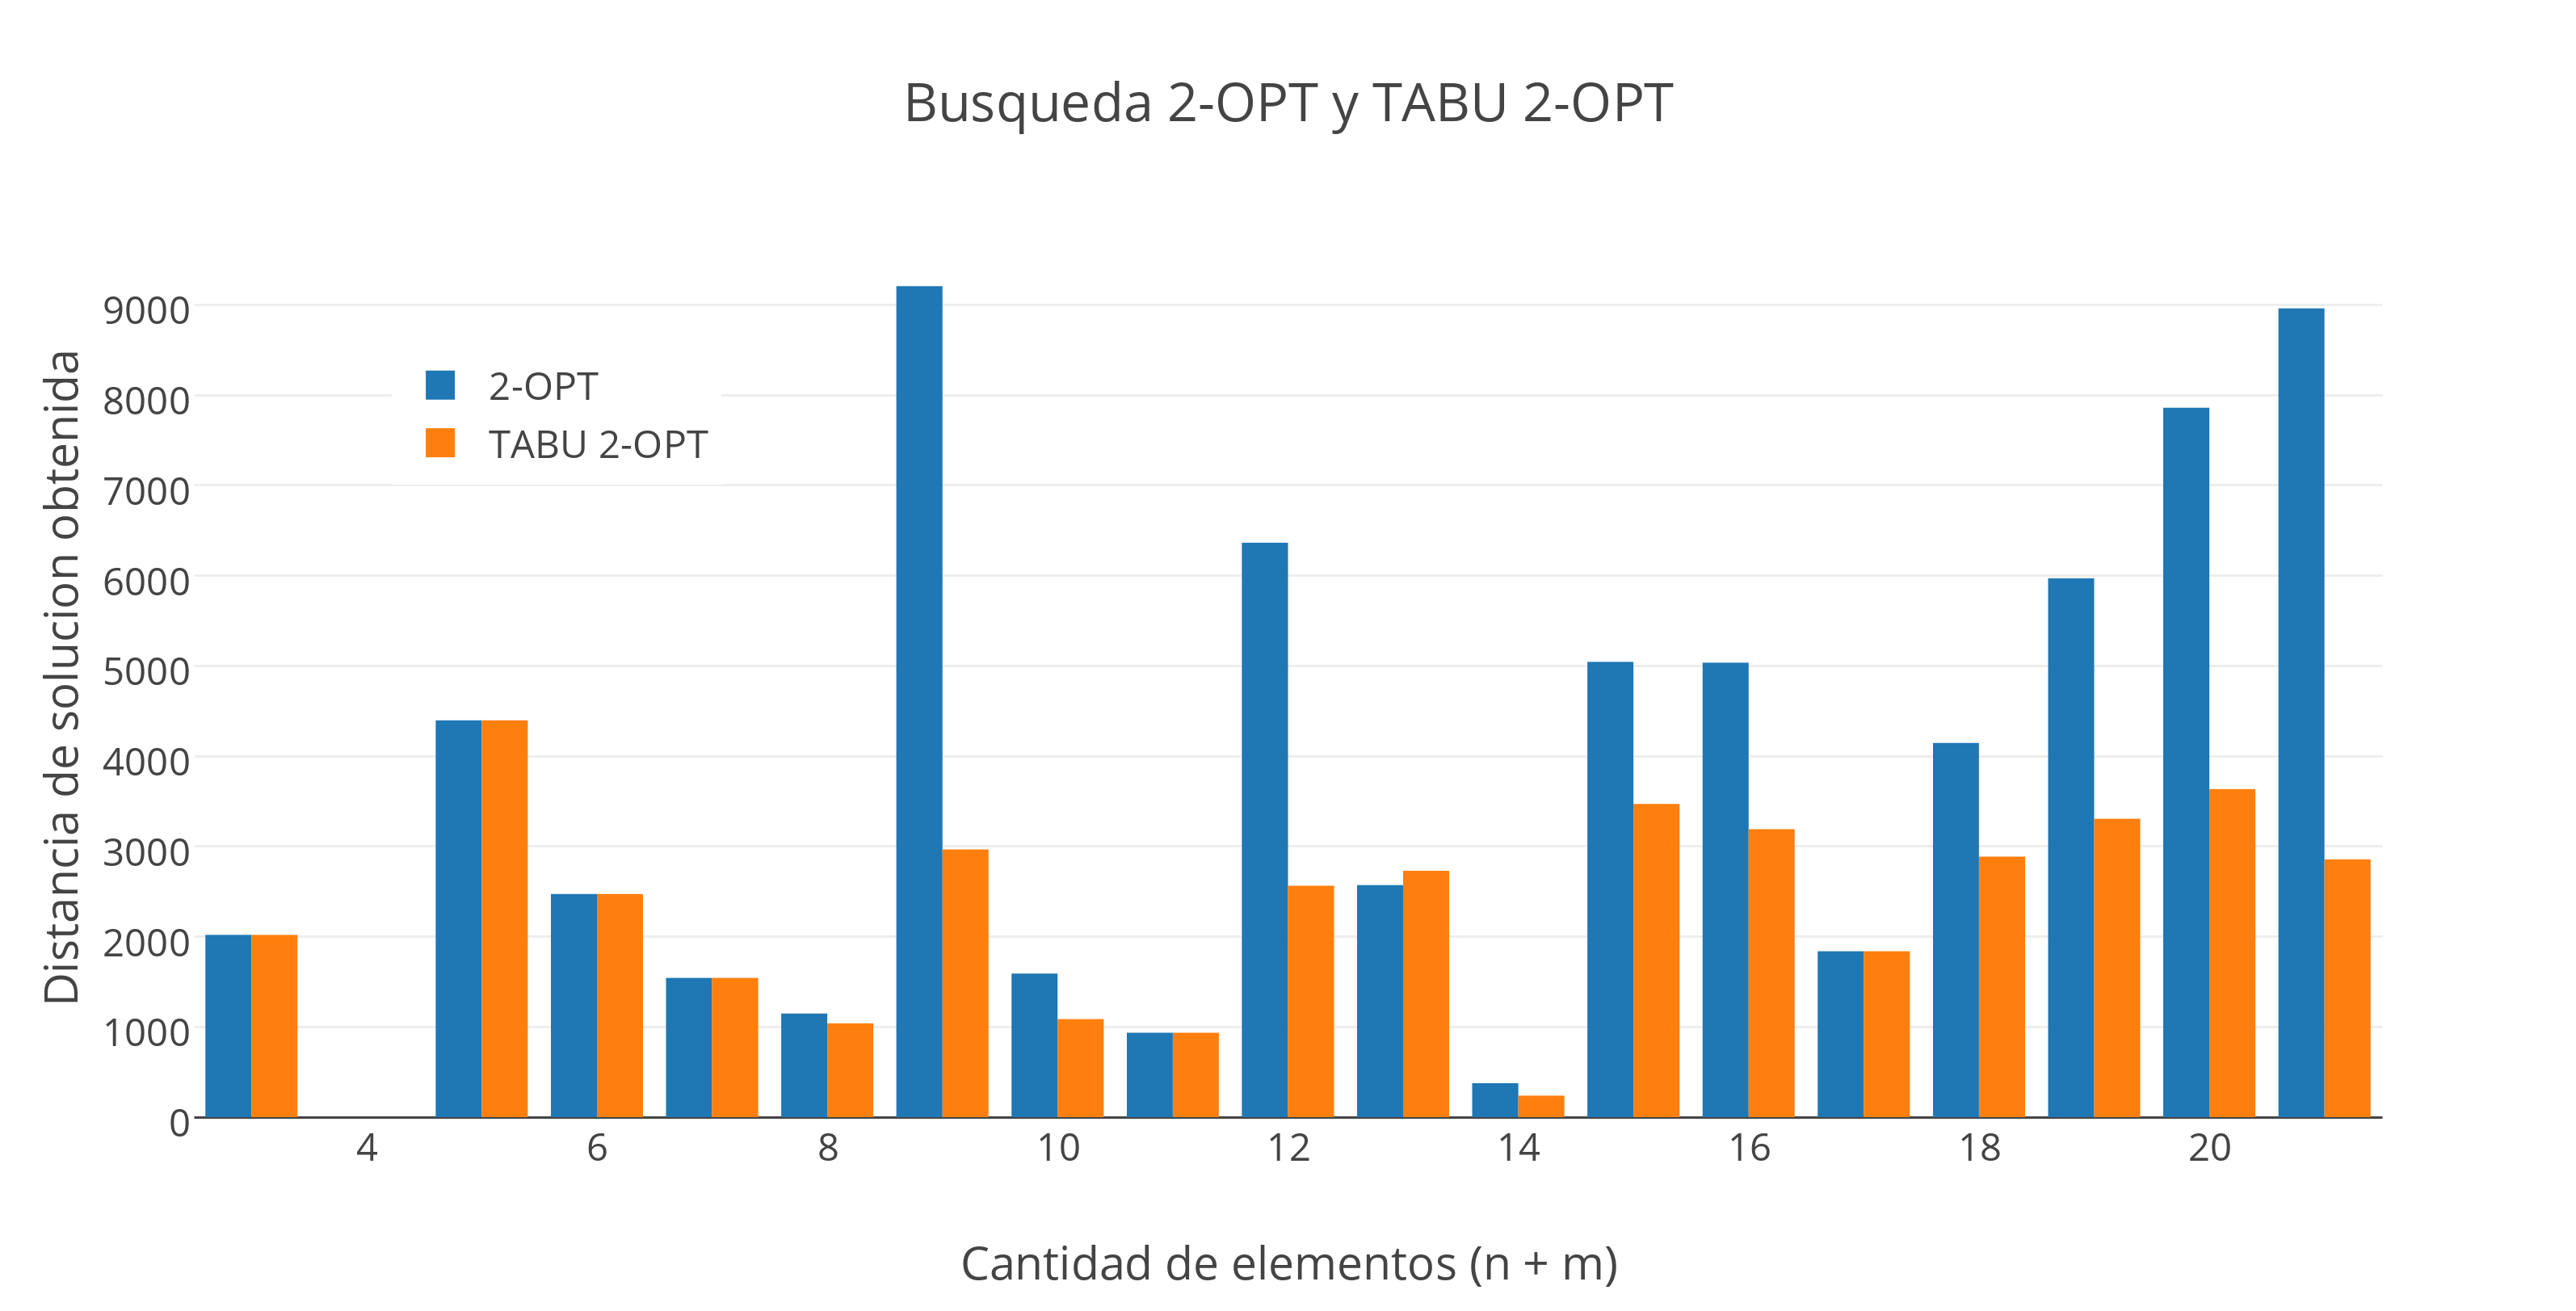
\includegraphics[scale=0.5]{./EJ4/comparativorandom2opt.png}\\
 {            \textit{Gráfico \ 4.7 - 2-OPT vs Tabu 2-OPT sobre Familia 8}}
  \end{center}
  \vspace*{0.3cm}

En cuanto a tiempo insumido vemos lo siguiente:

\vspace*{0.3cm} \vspace*{0.3cm}
  \begin{center}
 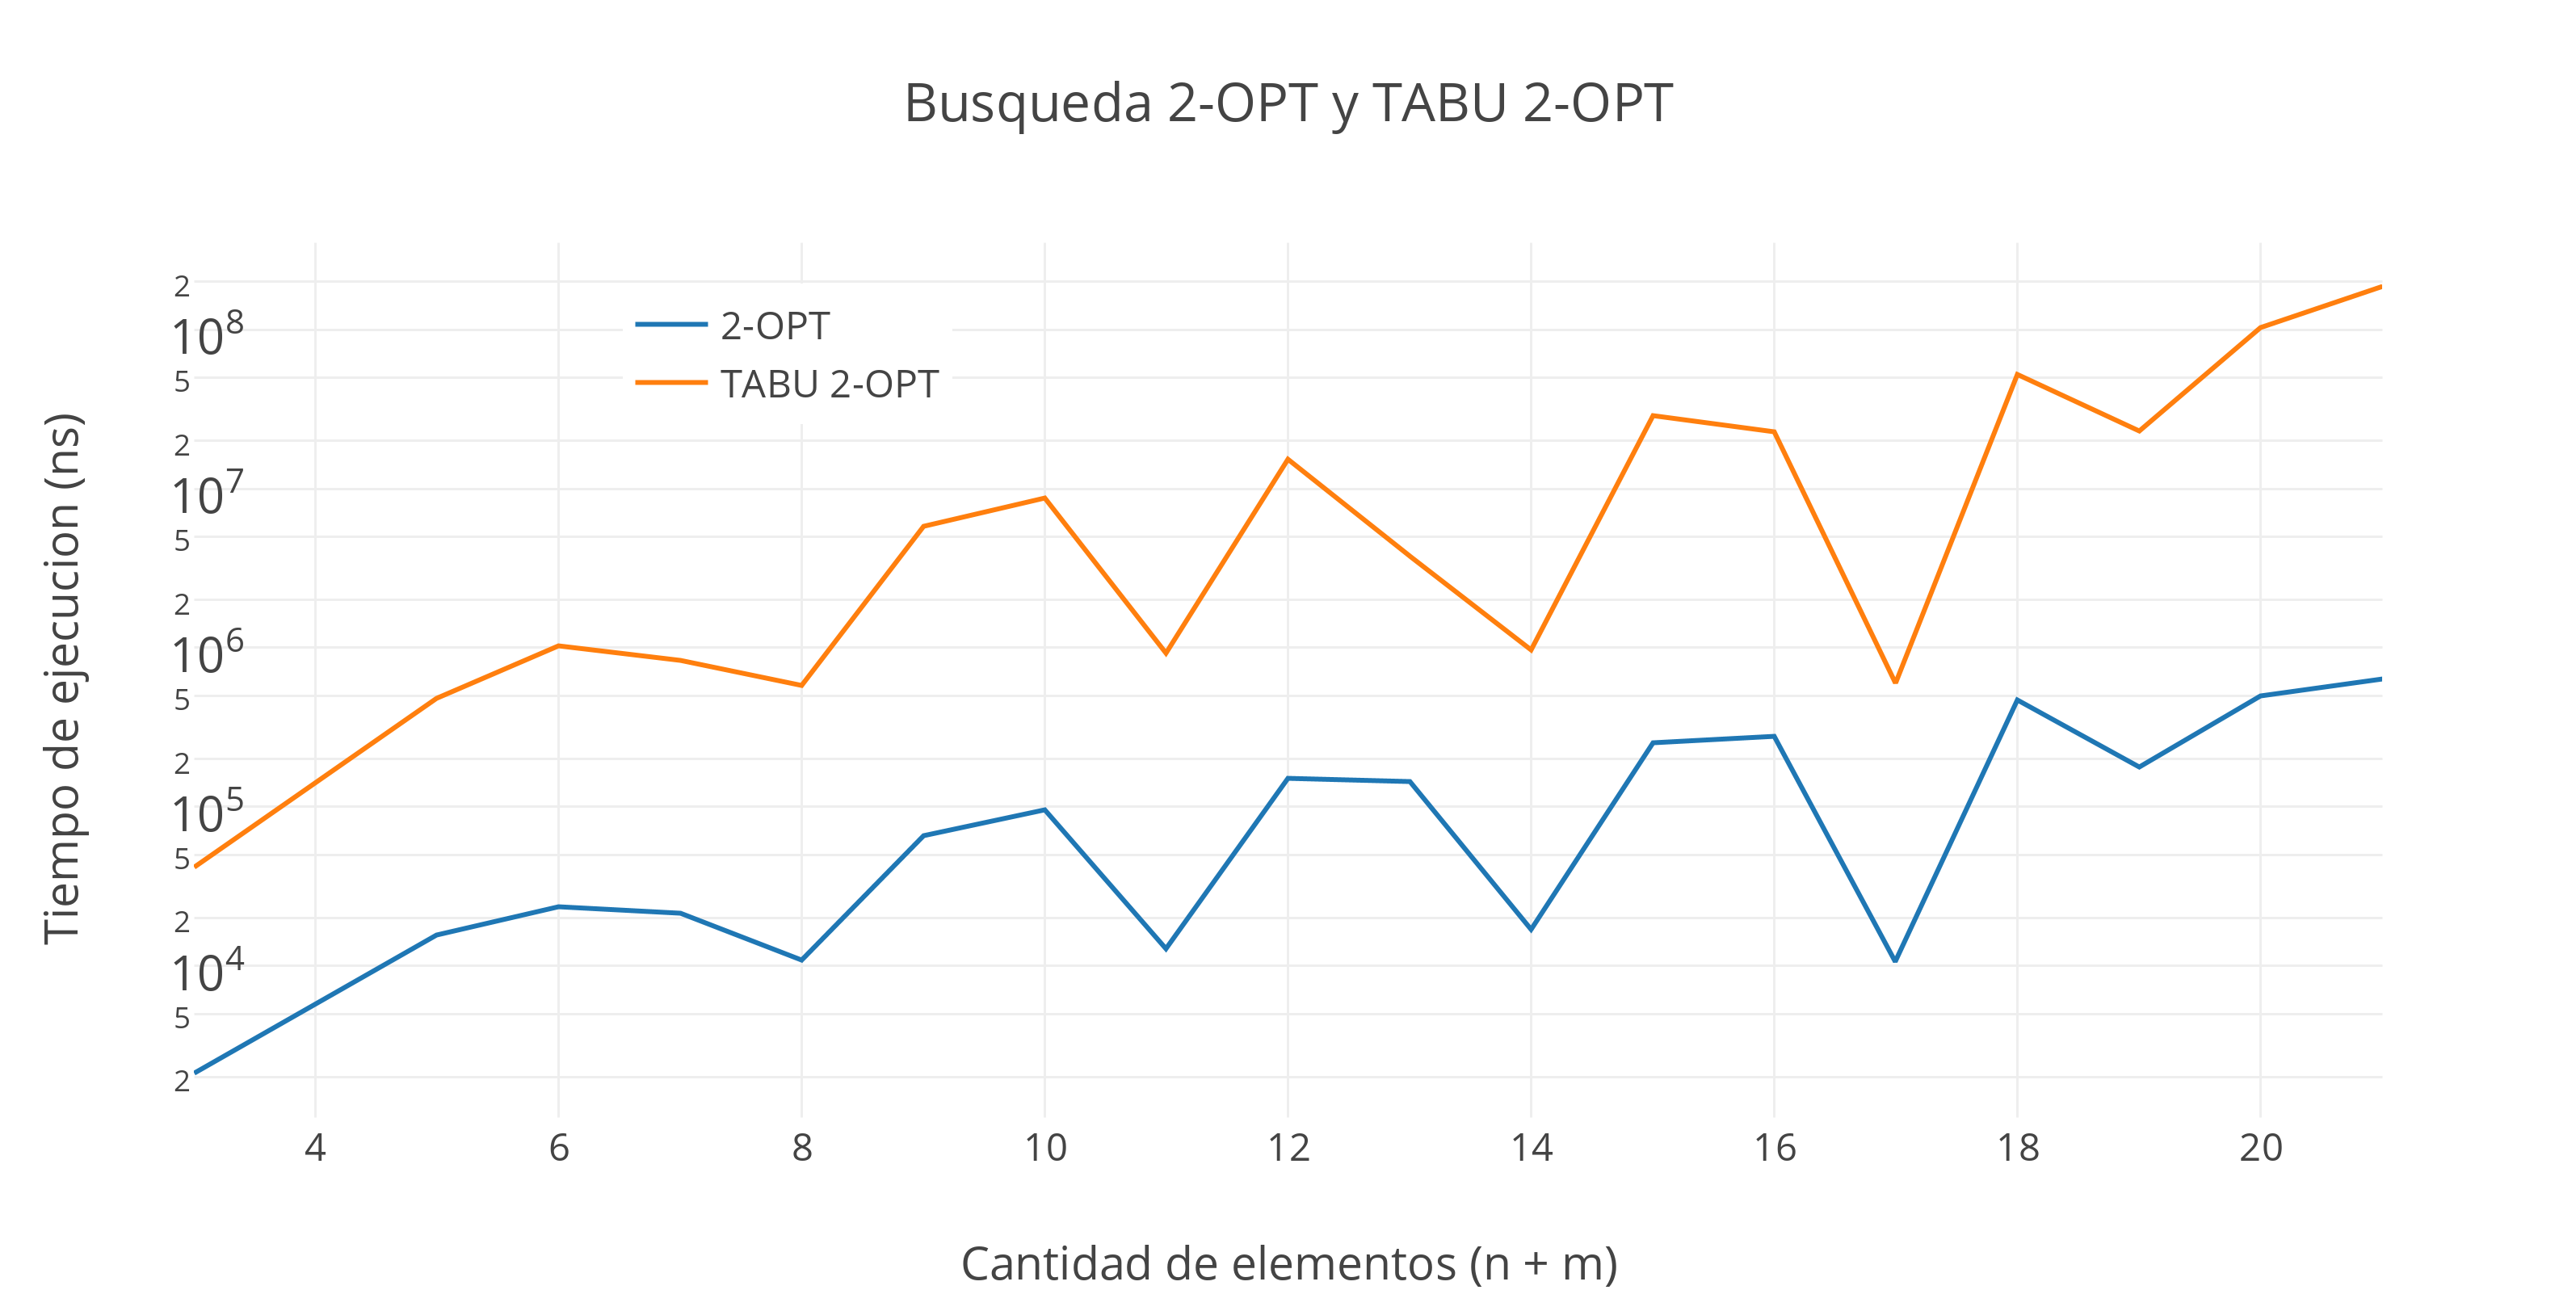
\includegraphics[scale=0.5]{./EJ4/medicionrandom2opt.png}\\
 {            \textit{Gráfico \ 4.8 - 2-OPT vs Tabu 2-OPT sobre Familia 6}}
  \end{center}
  \vspace*{0.3cm}


Luego, para 3-OPT:

\vspace*{0.3cm} \vspace*{0.3cm}
  \begin{center}
 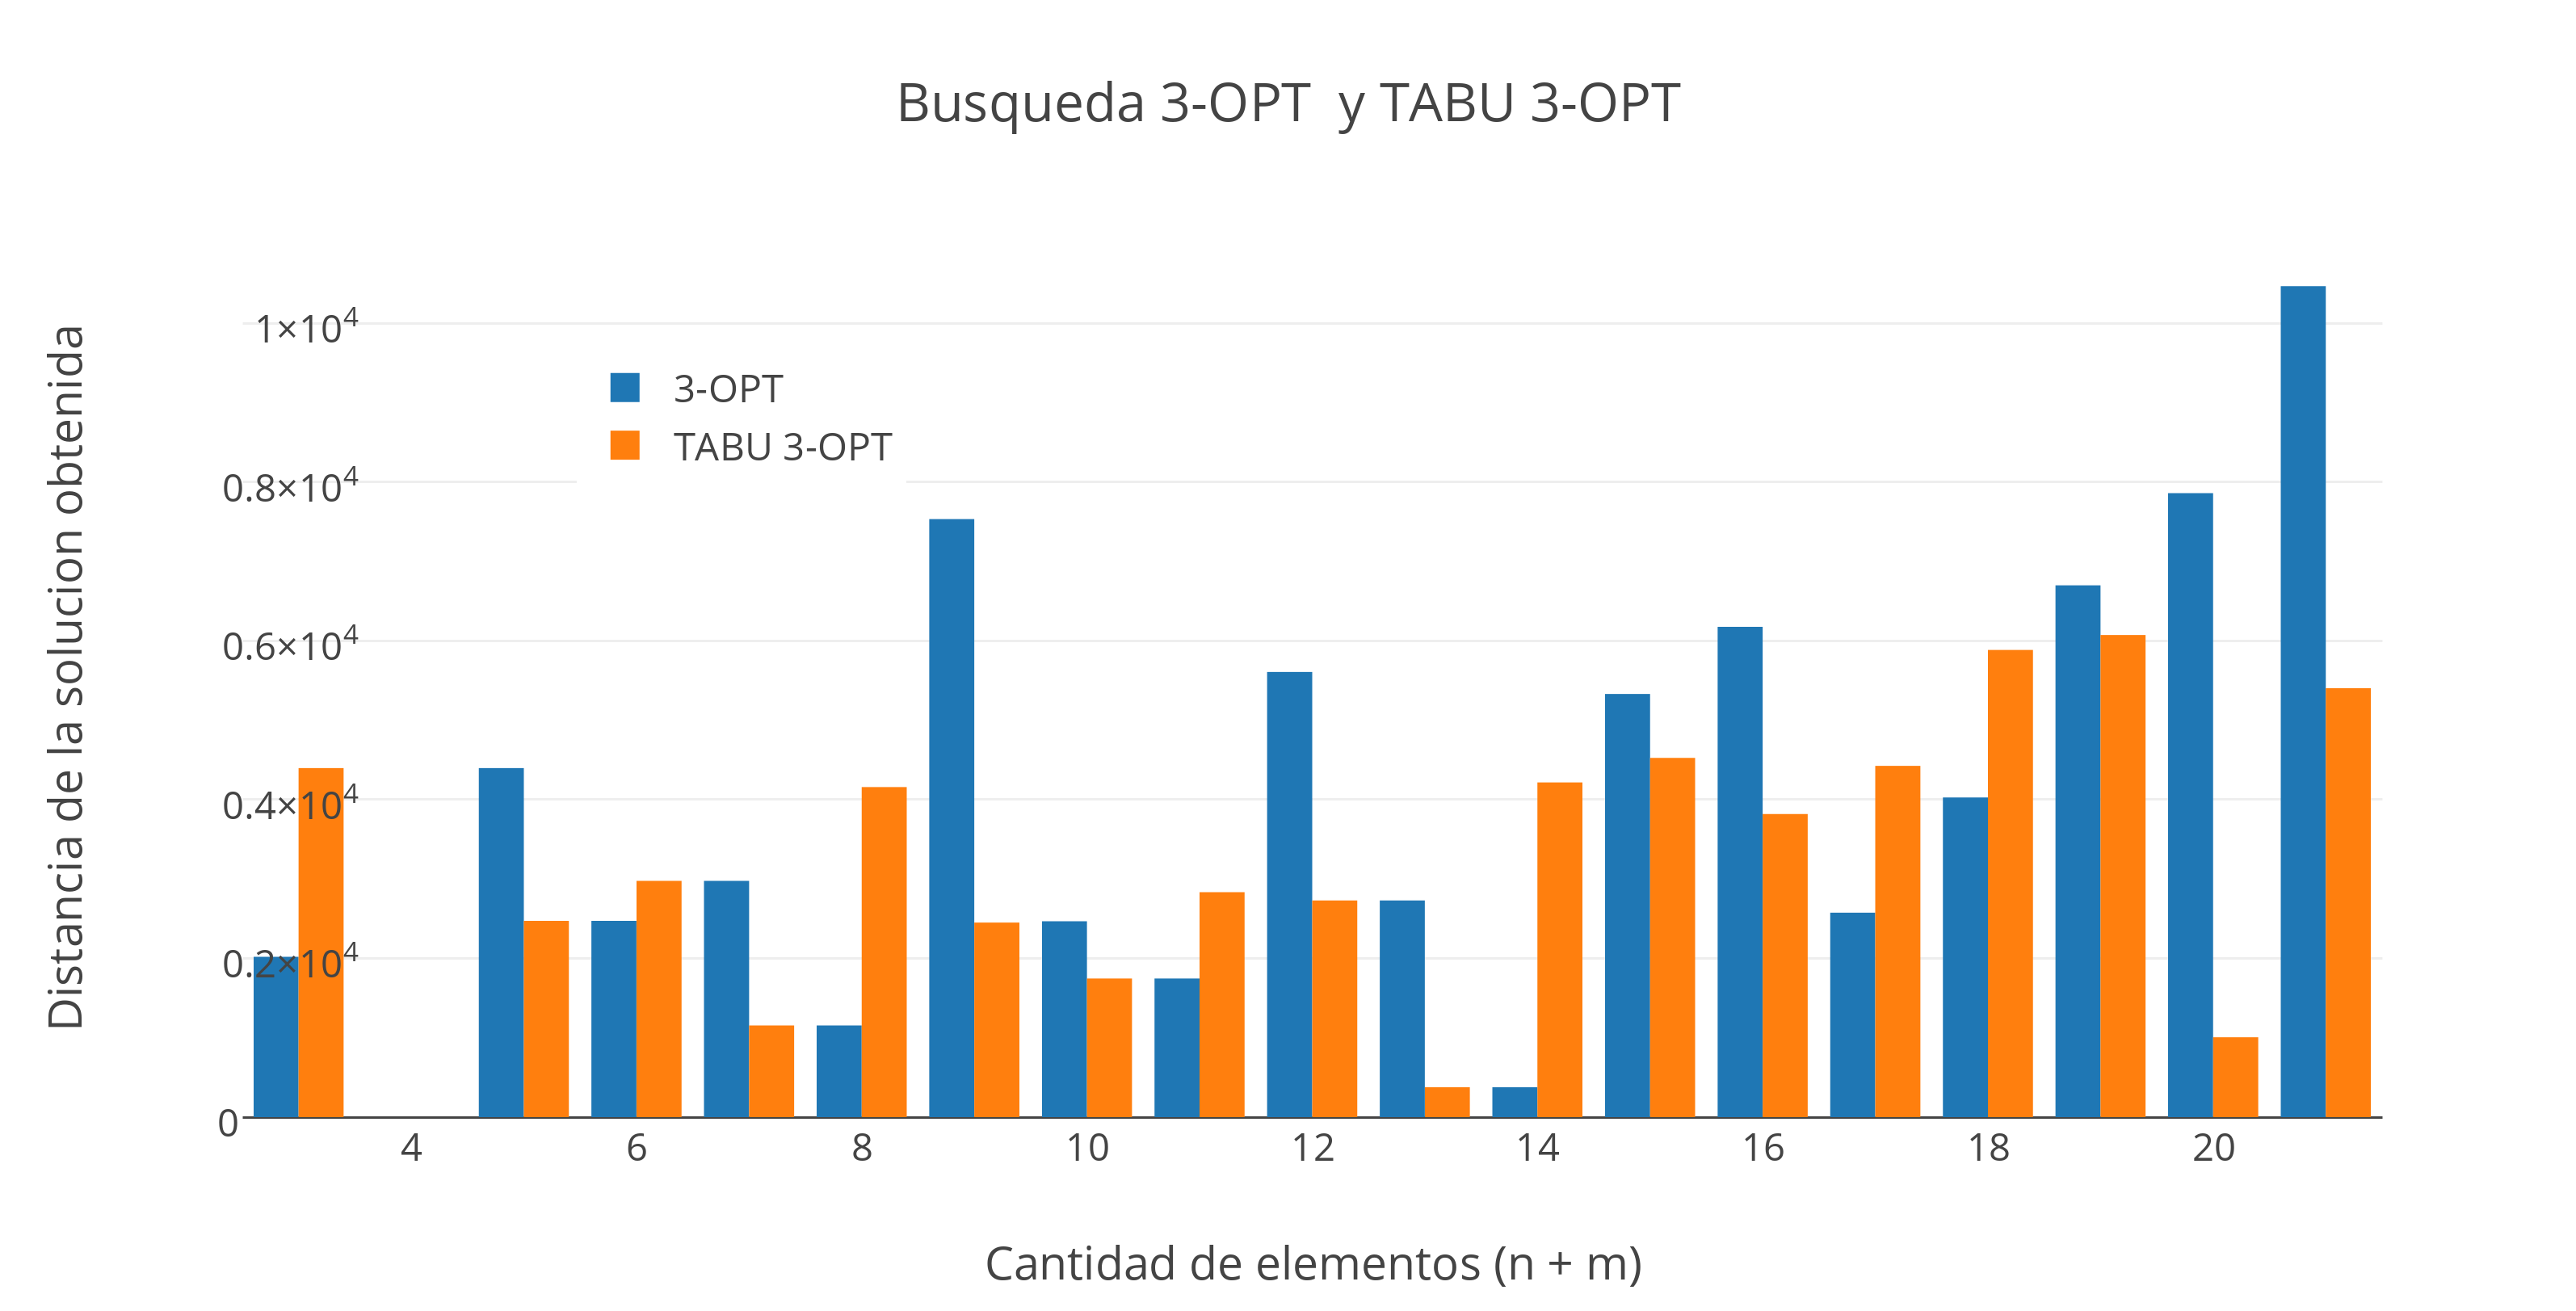
\includegraphics[scale=0.5]{./EJ4/comparativorandom3opt.png}\\
 {            \textit{Gráfico \ 4.9 - 3-OPT vs Tabu 3-OPT sobre Familia 6}}
  \end{center}
  \vspace*{0.3cm}

En cuanto a tiempo insumido vemos lo siguiente:

\vspace*{0.3cm} \vspace*{0.3cm}
  \begin{center}
 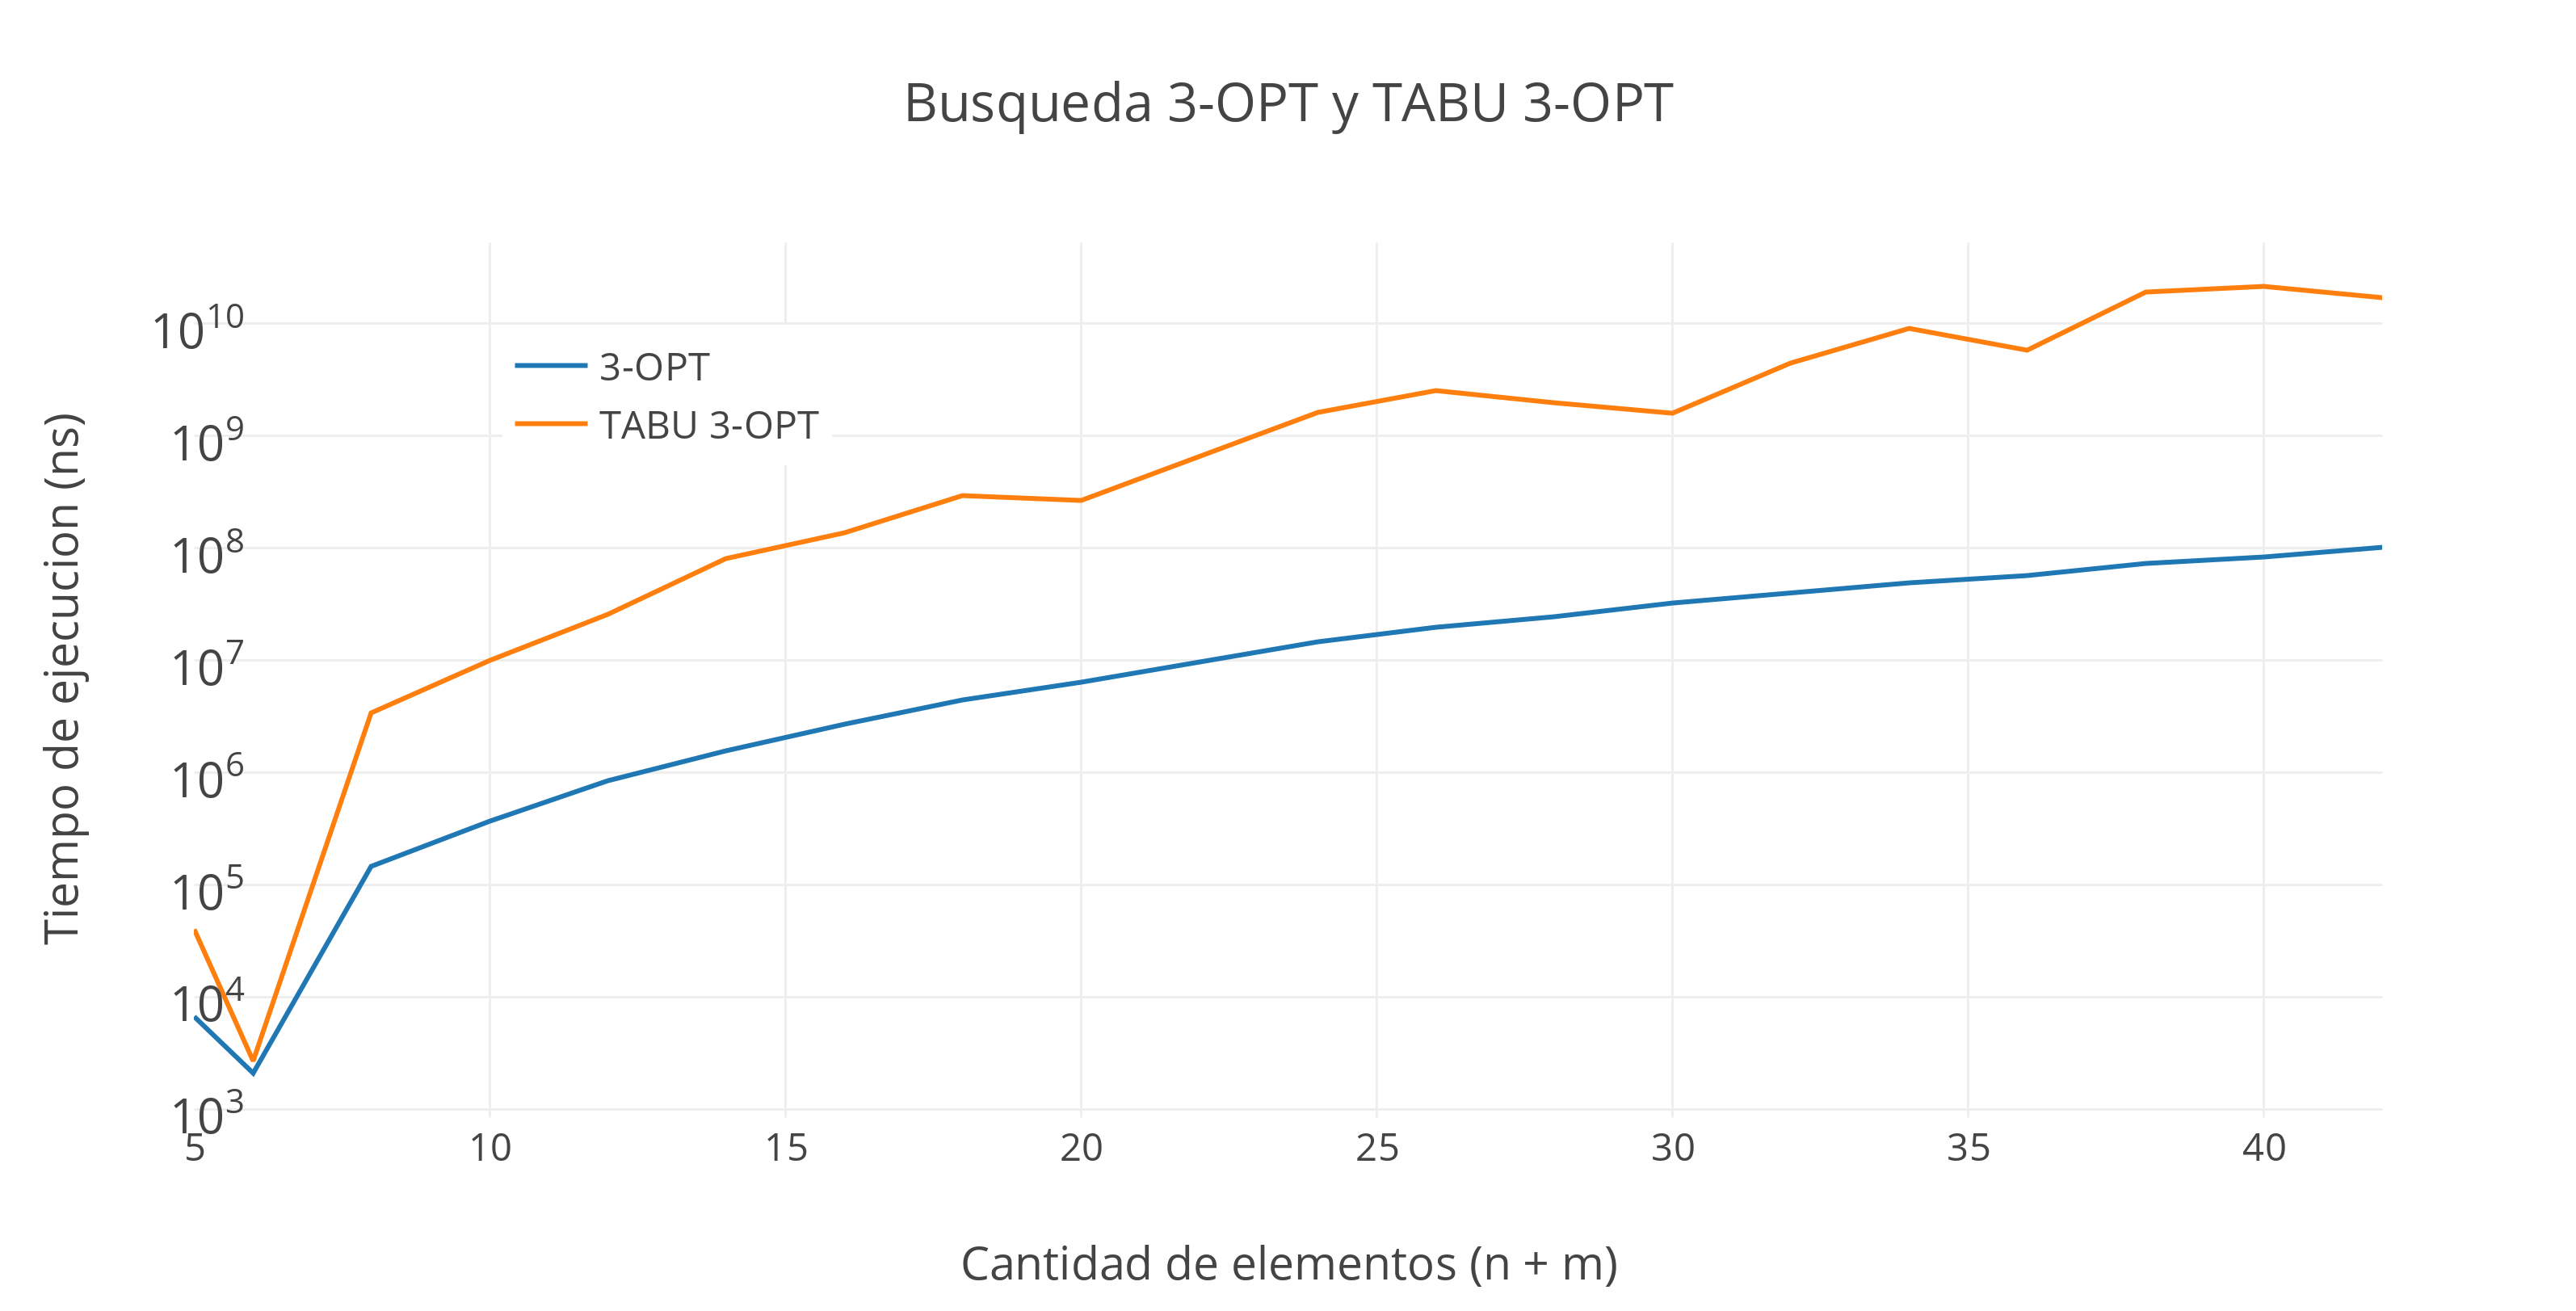
\includegraphics[scale=0.5]{./EJ4/medicionrandom3opt.png}\\
 {            \textit{Gráfico \ 4.10 - 3-OPT vs Tabu 3-OPT sobre Familia 6}}
  \end{center}
  \vspace*{0.3cm}
  
Para la comparación entre algoritmos tabu, se comparará conjuntamente el tiempo de ejecución con la calidad de la solución. Para esta última tendremos en cuenta que los algoritmos, de devolver un resultado, será válido: esto quiere decir que cuanto menor distancia recorran en las soluciones, mejor serán las mismas:

Las soluciones obtenidas fueron las siguientes:

\vspace*{0.3cm} \vspace*{0.3cm}
  \begin{center}
 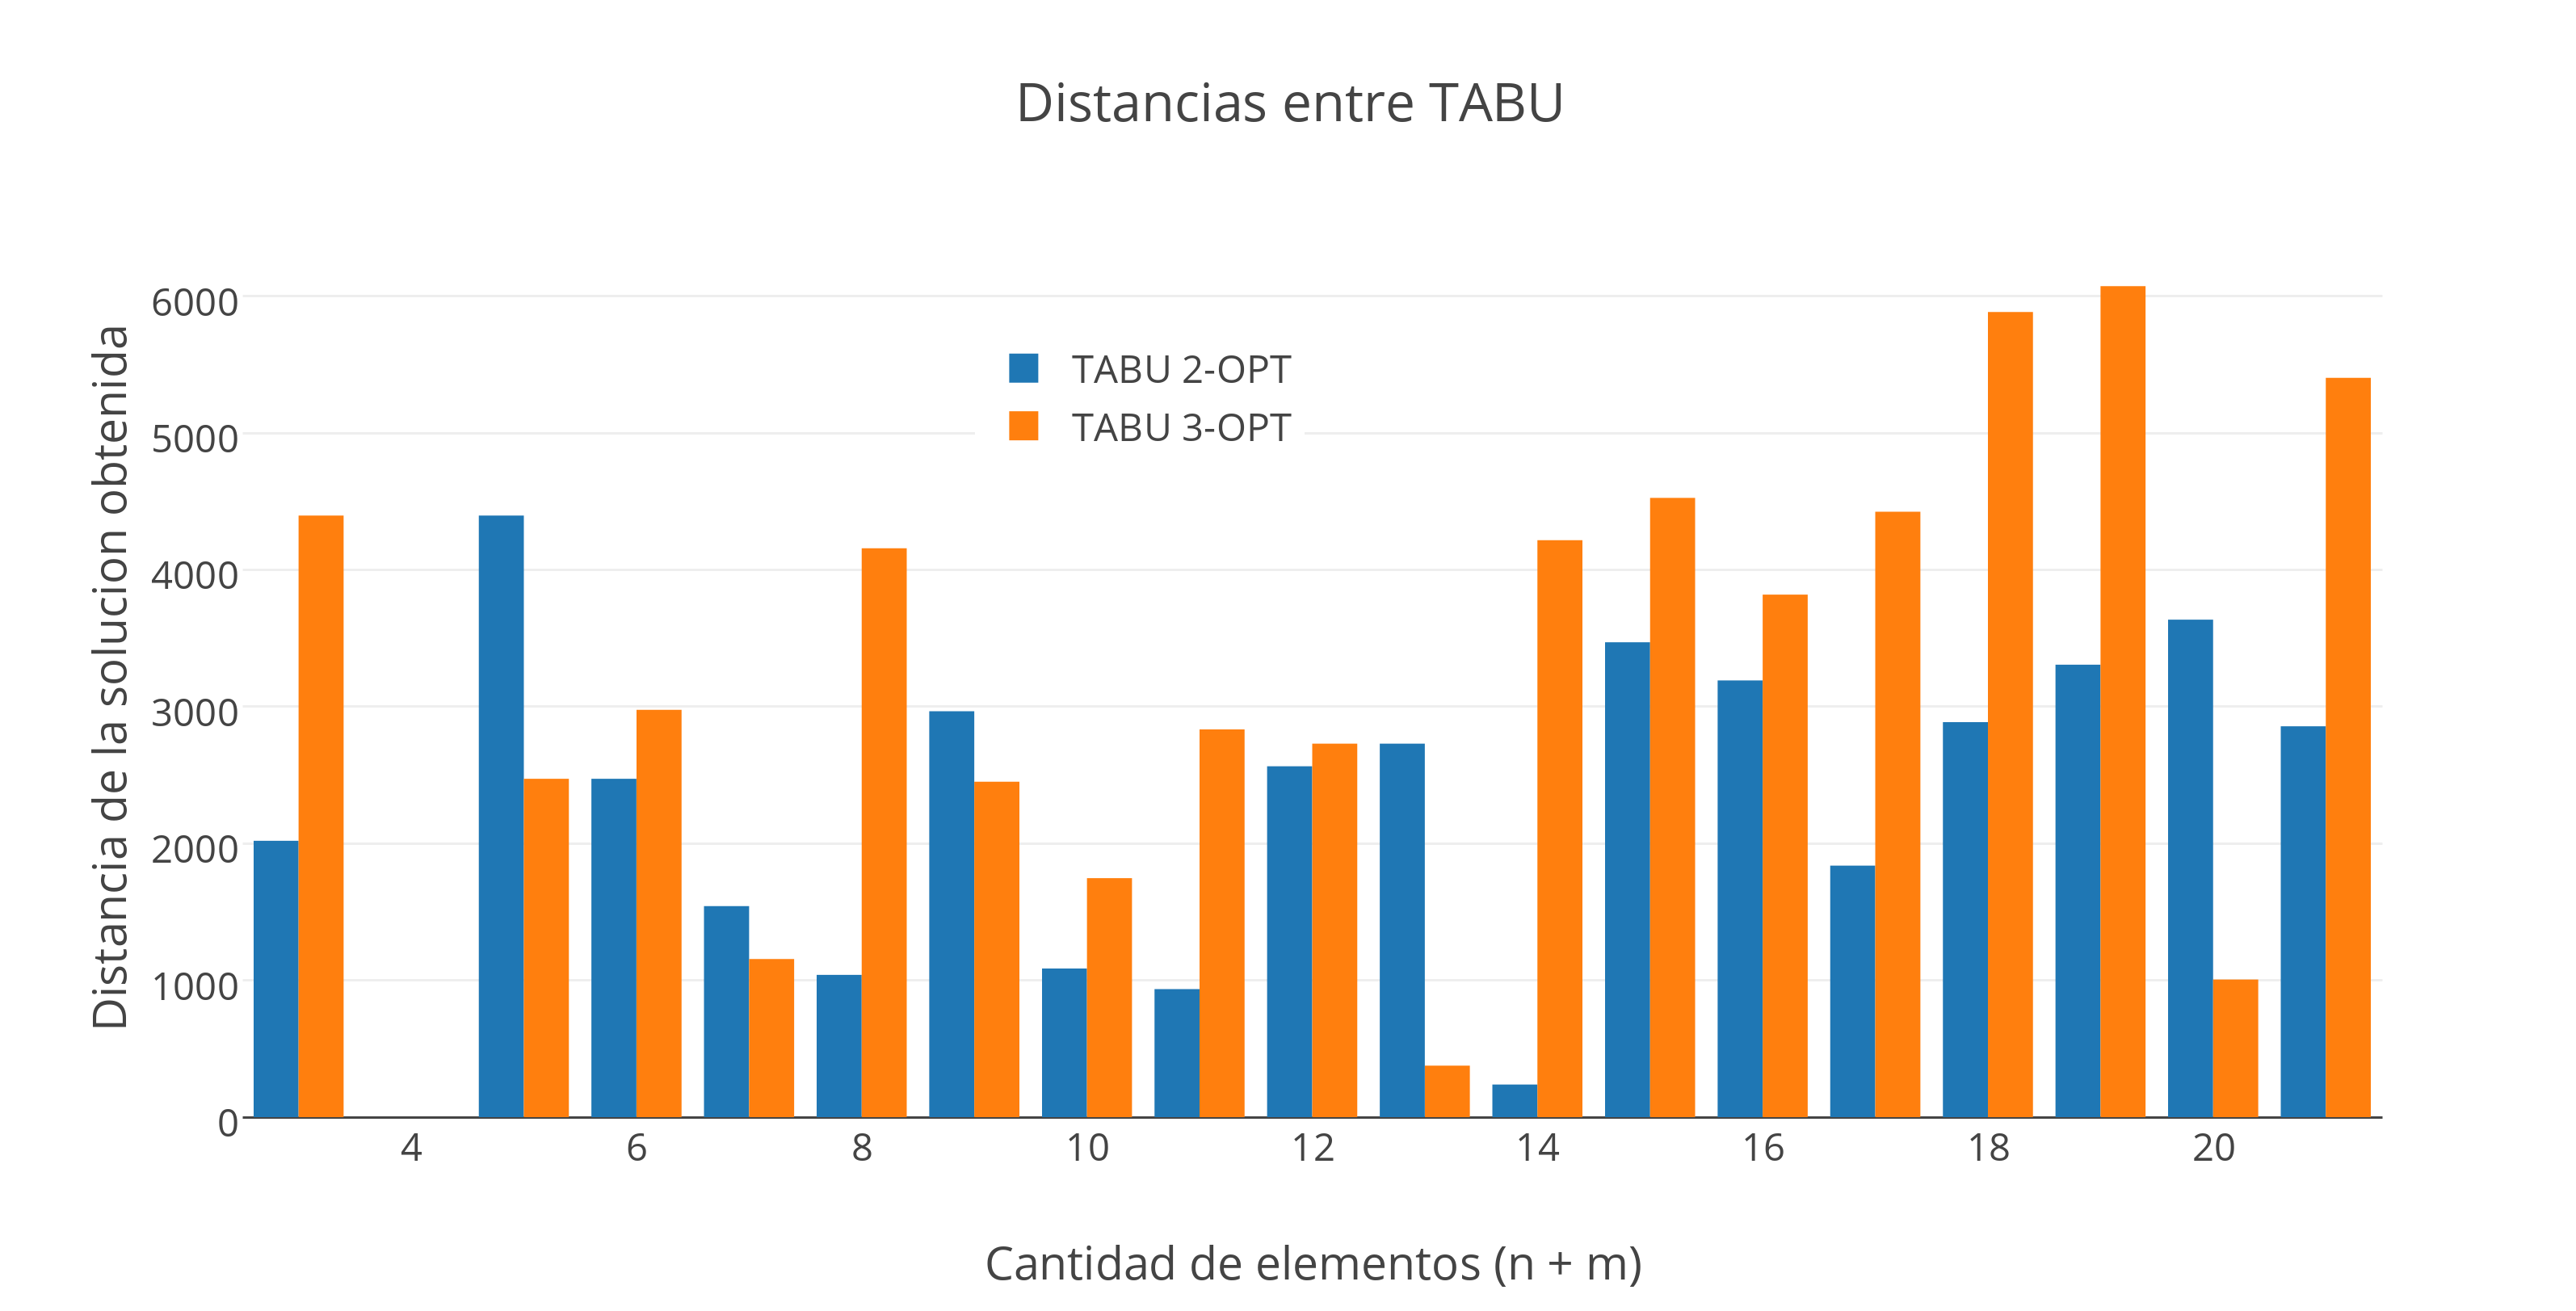
\includegraphics[scale=0.5]{./EJ4/comparativorandom.png}\\
 {            \textit{Gráfico \ 4.11 - Tabu 2-OPT vs Tabu 3-OPT sobre Familia 6}}
  \end{center}
  \vspace*{0.3cm}

En cuanto a tiempo insumido vemos lo siguiente:

\vspace*{0.3cm} \vspace*{0.3cm}
  \begin{center}
 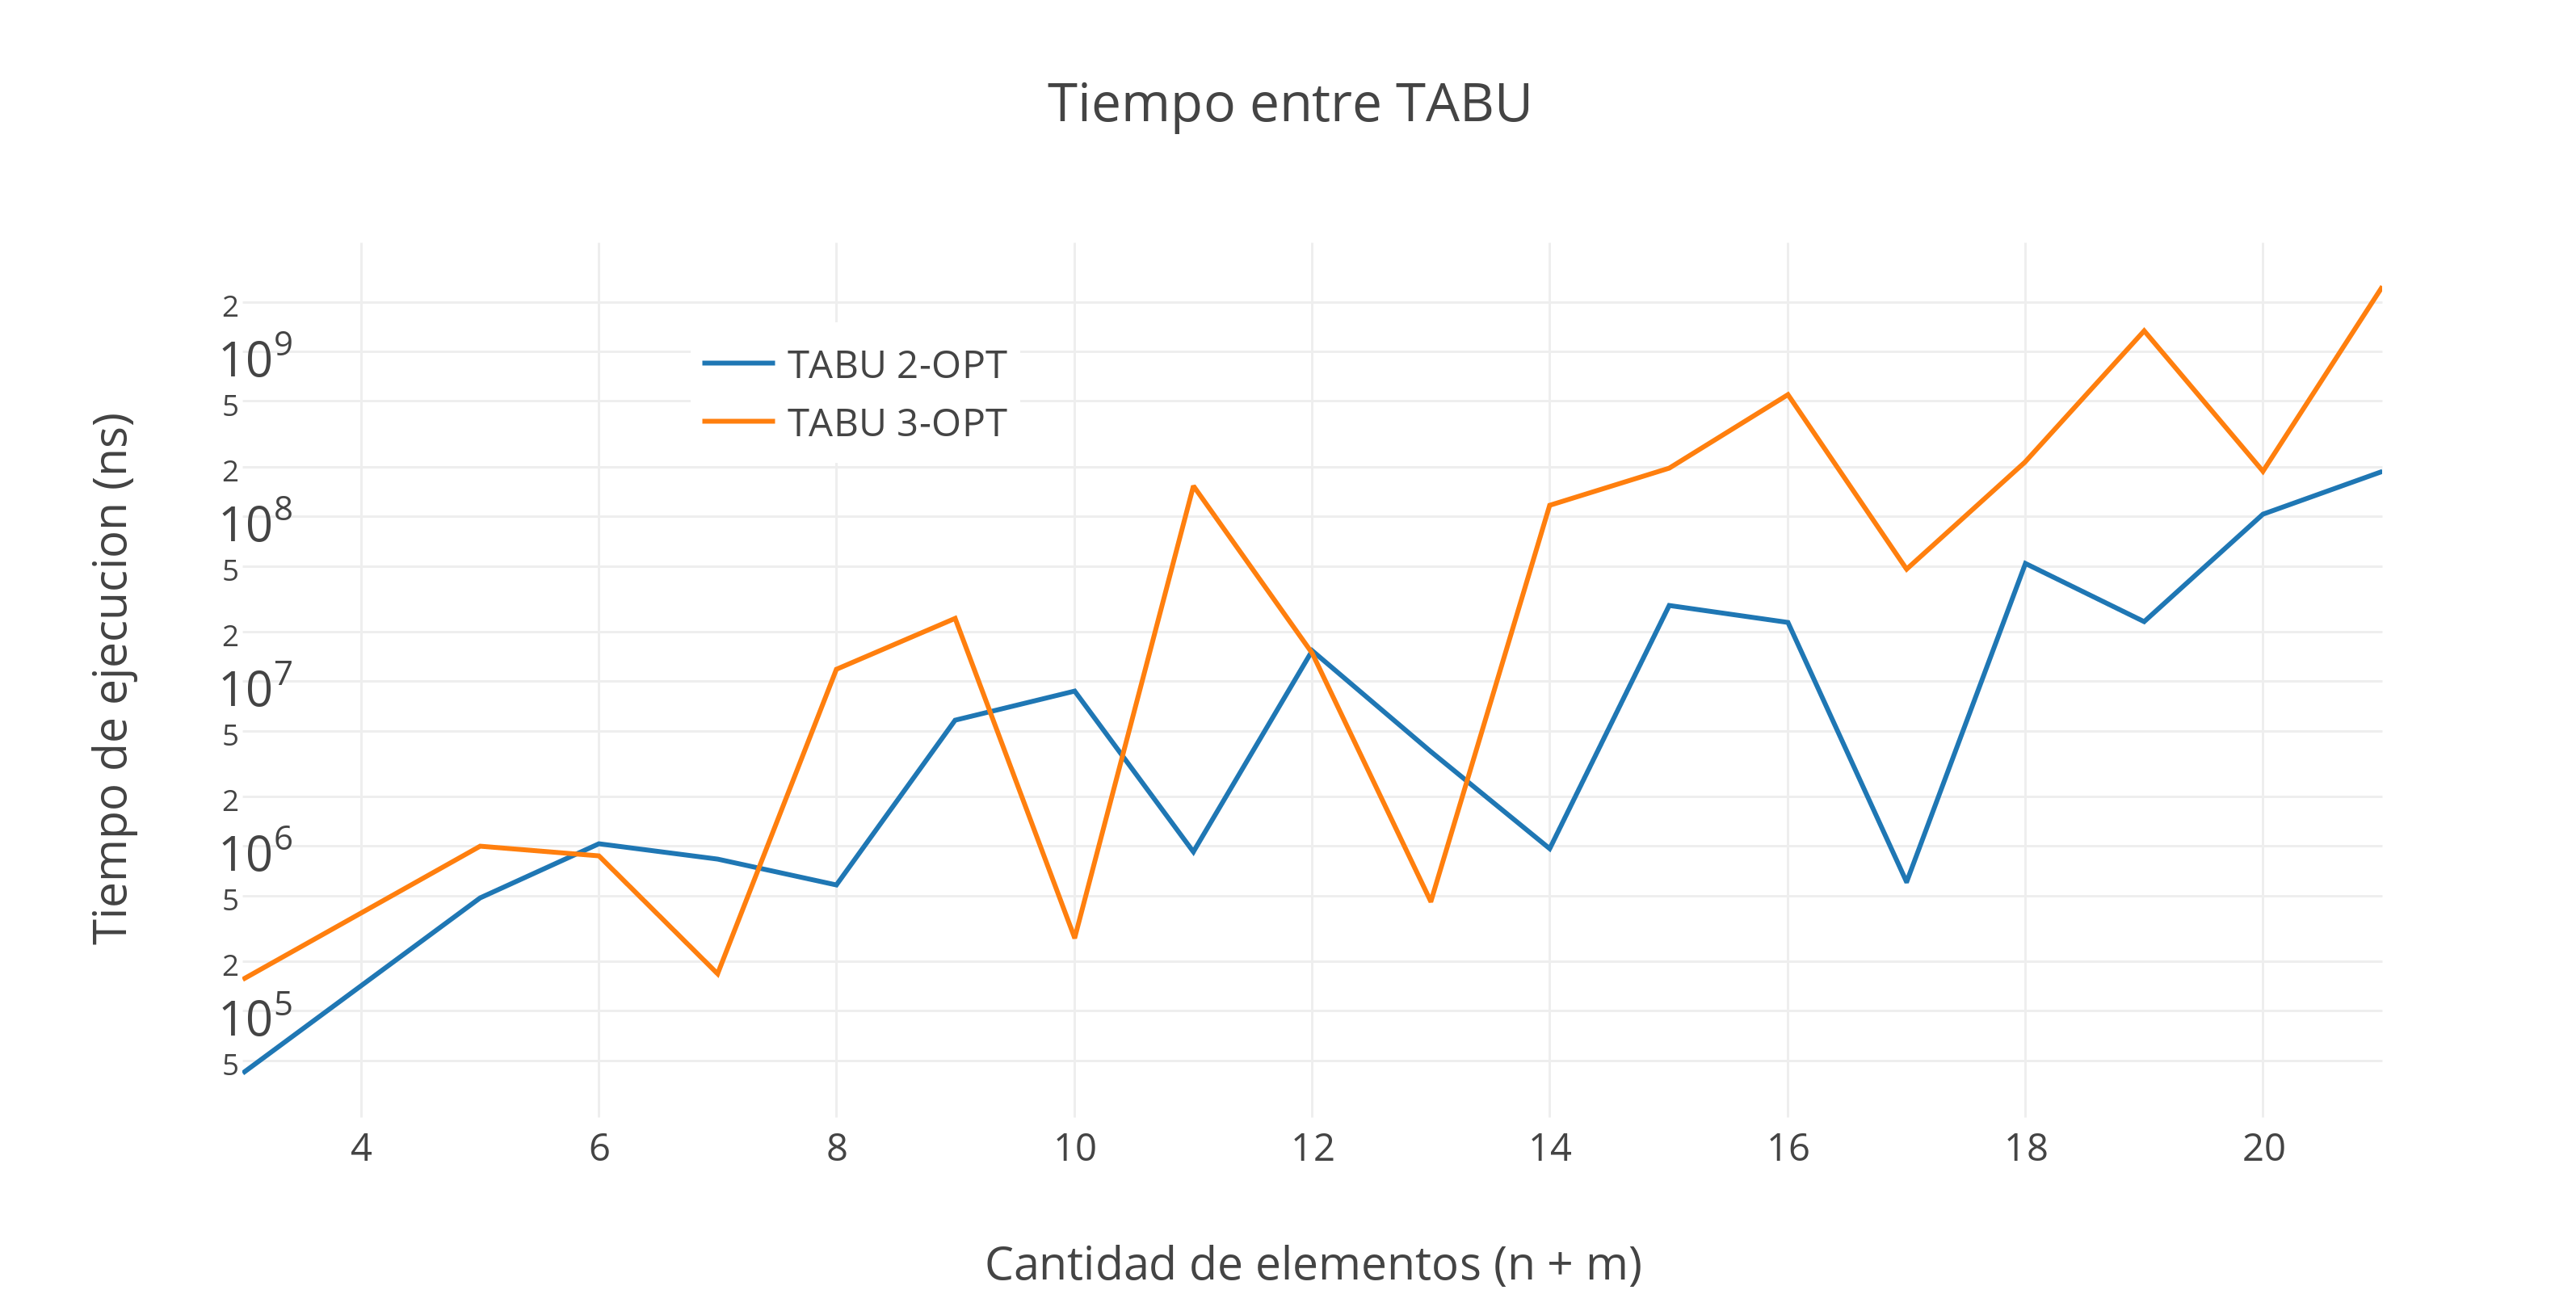
\includegraphics[scale=0.5]{./EJ4/medicionrandom.png}\\
 {            \textit{Gráfico \ 4.12 - Tabu 2-OPT vs Tabu 3-OPT sobre Familia 6}}
  \end{center}
  \vspace*{0.3cm}
  

Habiendo chequeado dichas mediciones de tiempo de los algoritmos, se pudo observar como 3-OPT presento una peor performance con las familias evaluadas. En relaci\'on a tiempo - calidad de soluci\'on el mejor termino siendo 2-OPT.

------> ACOMODAR
Las mejoras se producen:


\vspace*{0.3cm} \vspace*{0.3cm}
  \begin{center}
 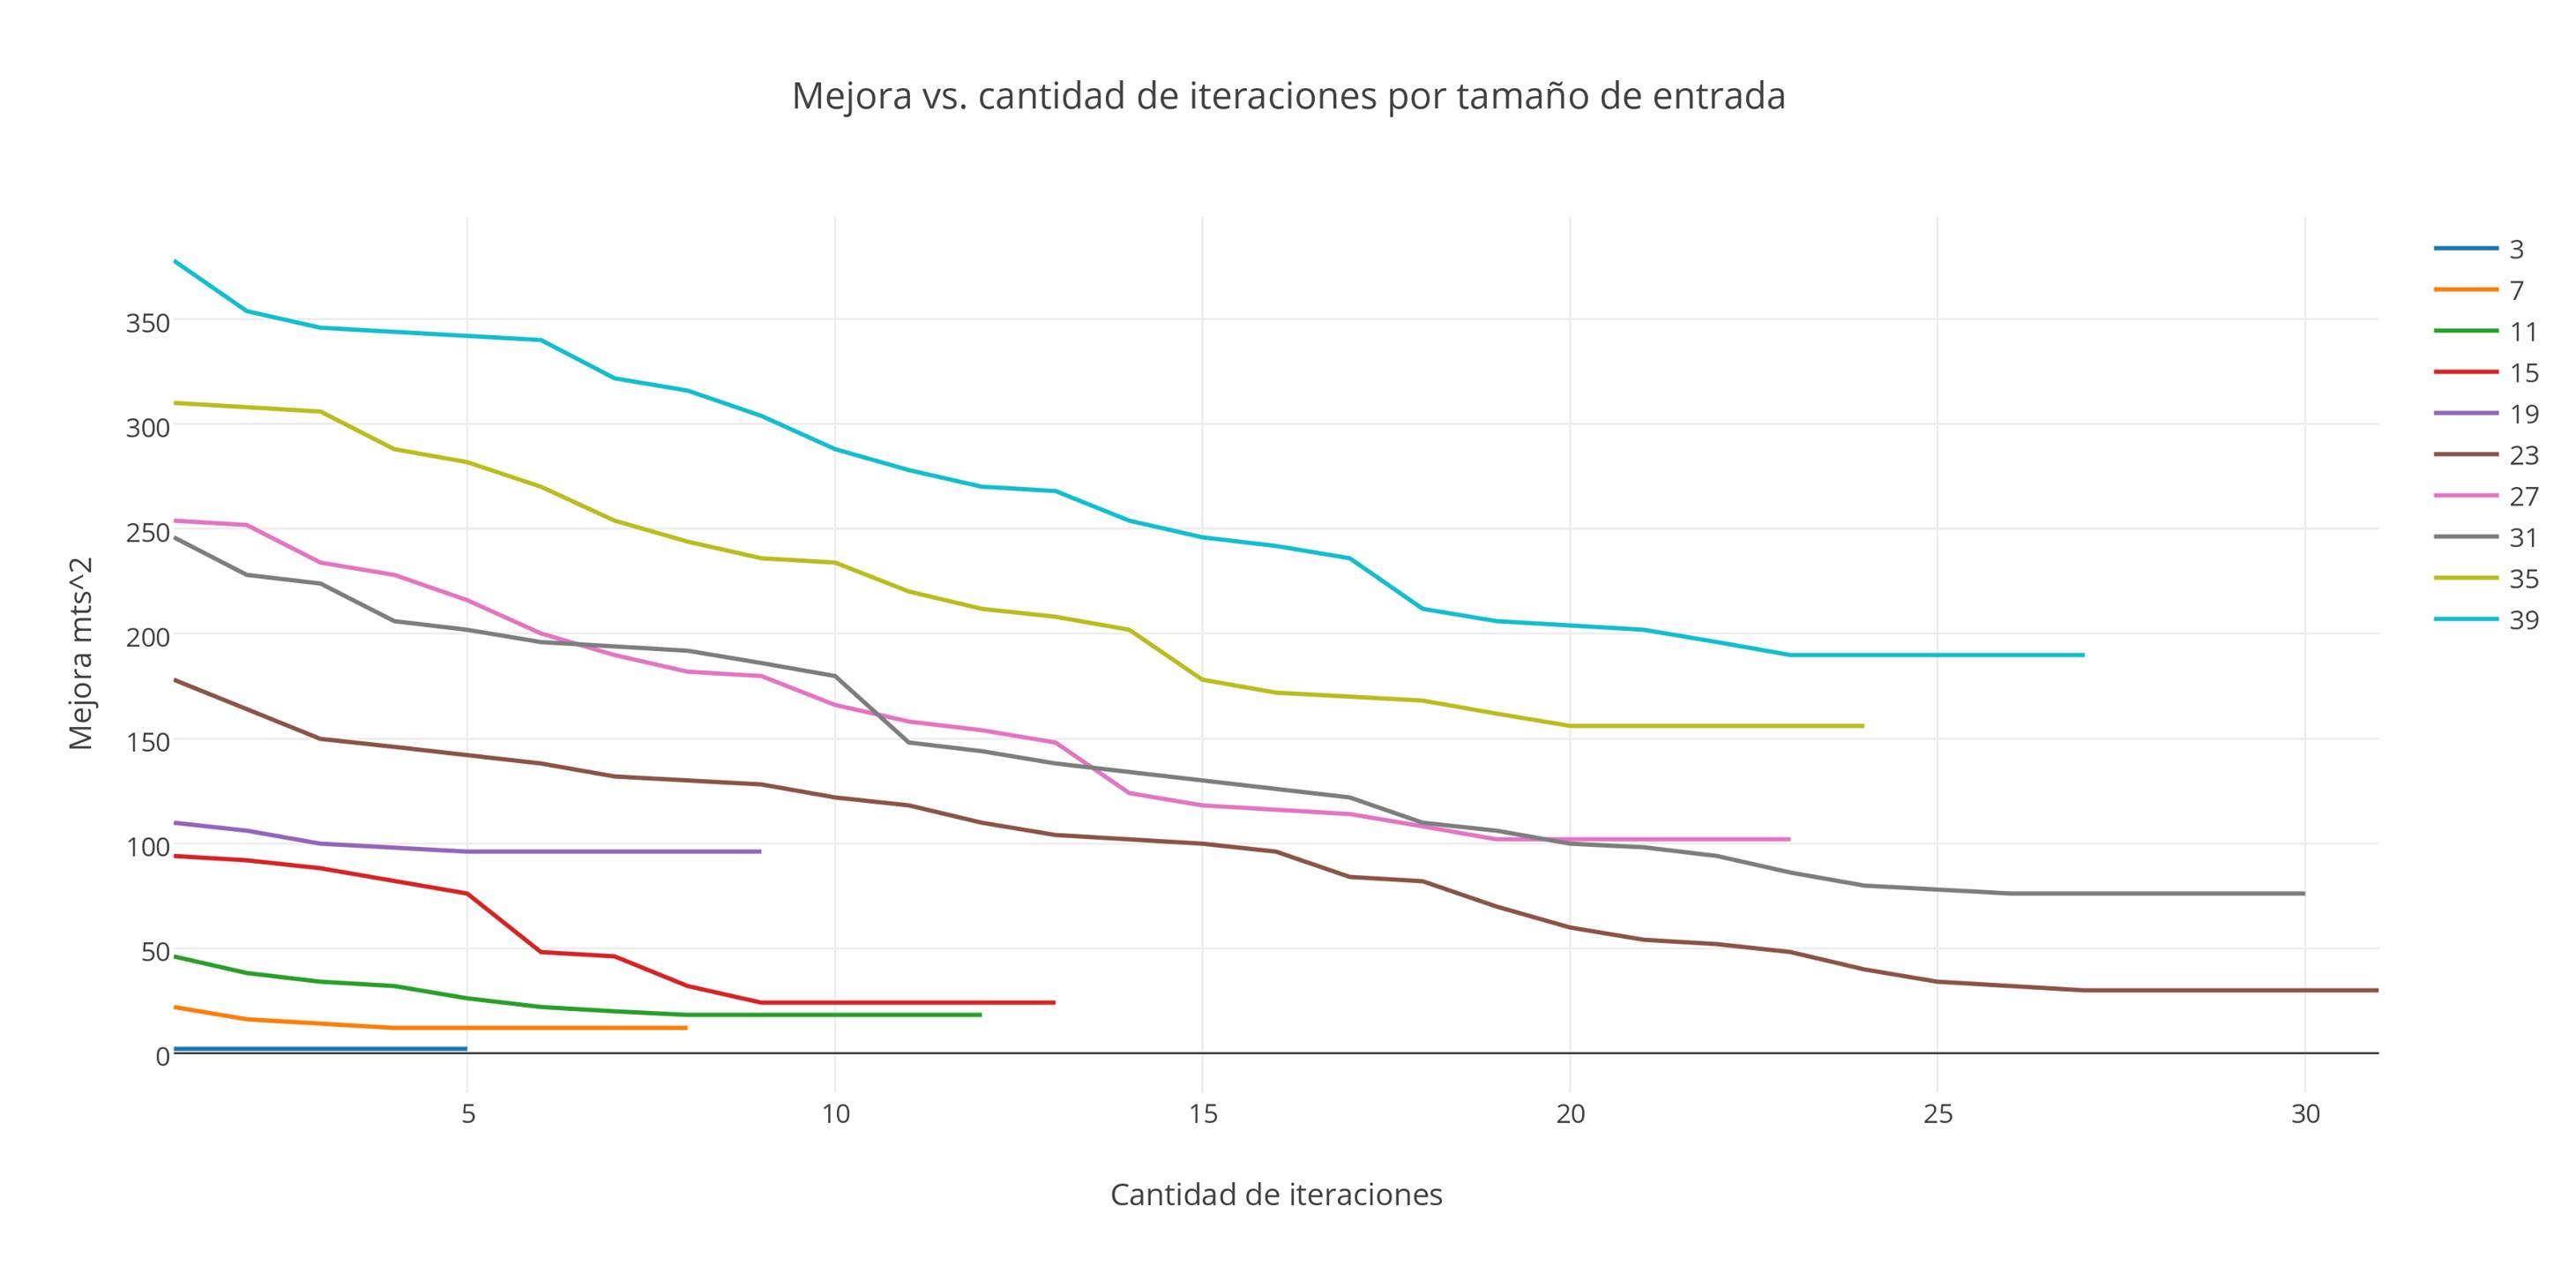
\includegraphics[scale=0.5]{./EJ4/mejora.png}\\
 {            \textit{Gráfico \ 4.12 - Tabu 2-OPT vs Tabu 3-OPT sobre Familia 6}}
  \end{center}
  \vspace*{0.3cm}
  
  \vspace*{0.3cm} \vspace*{0.3cm}
  \begin{center}
 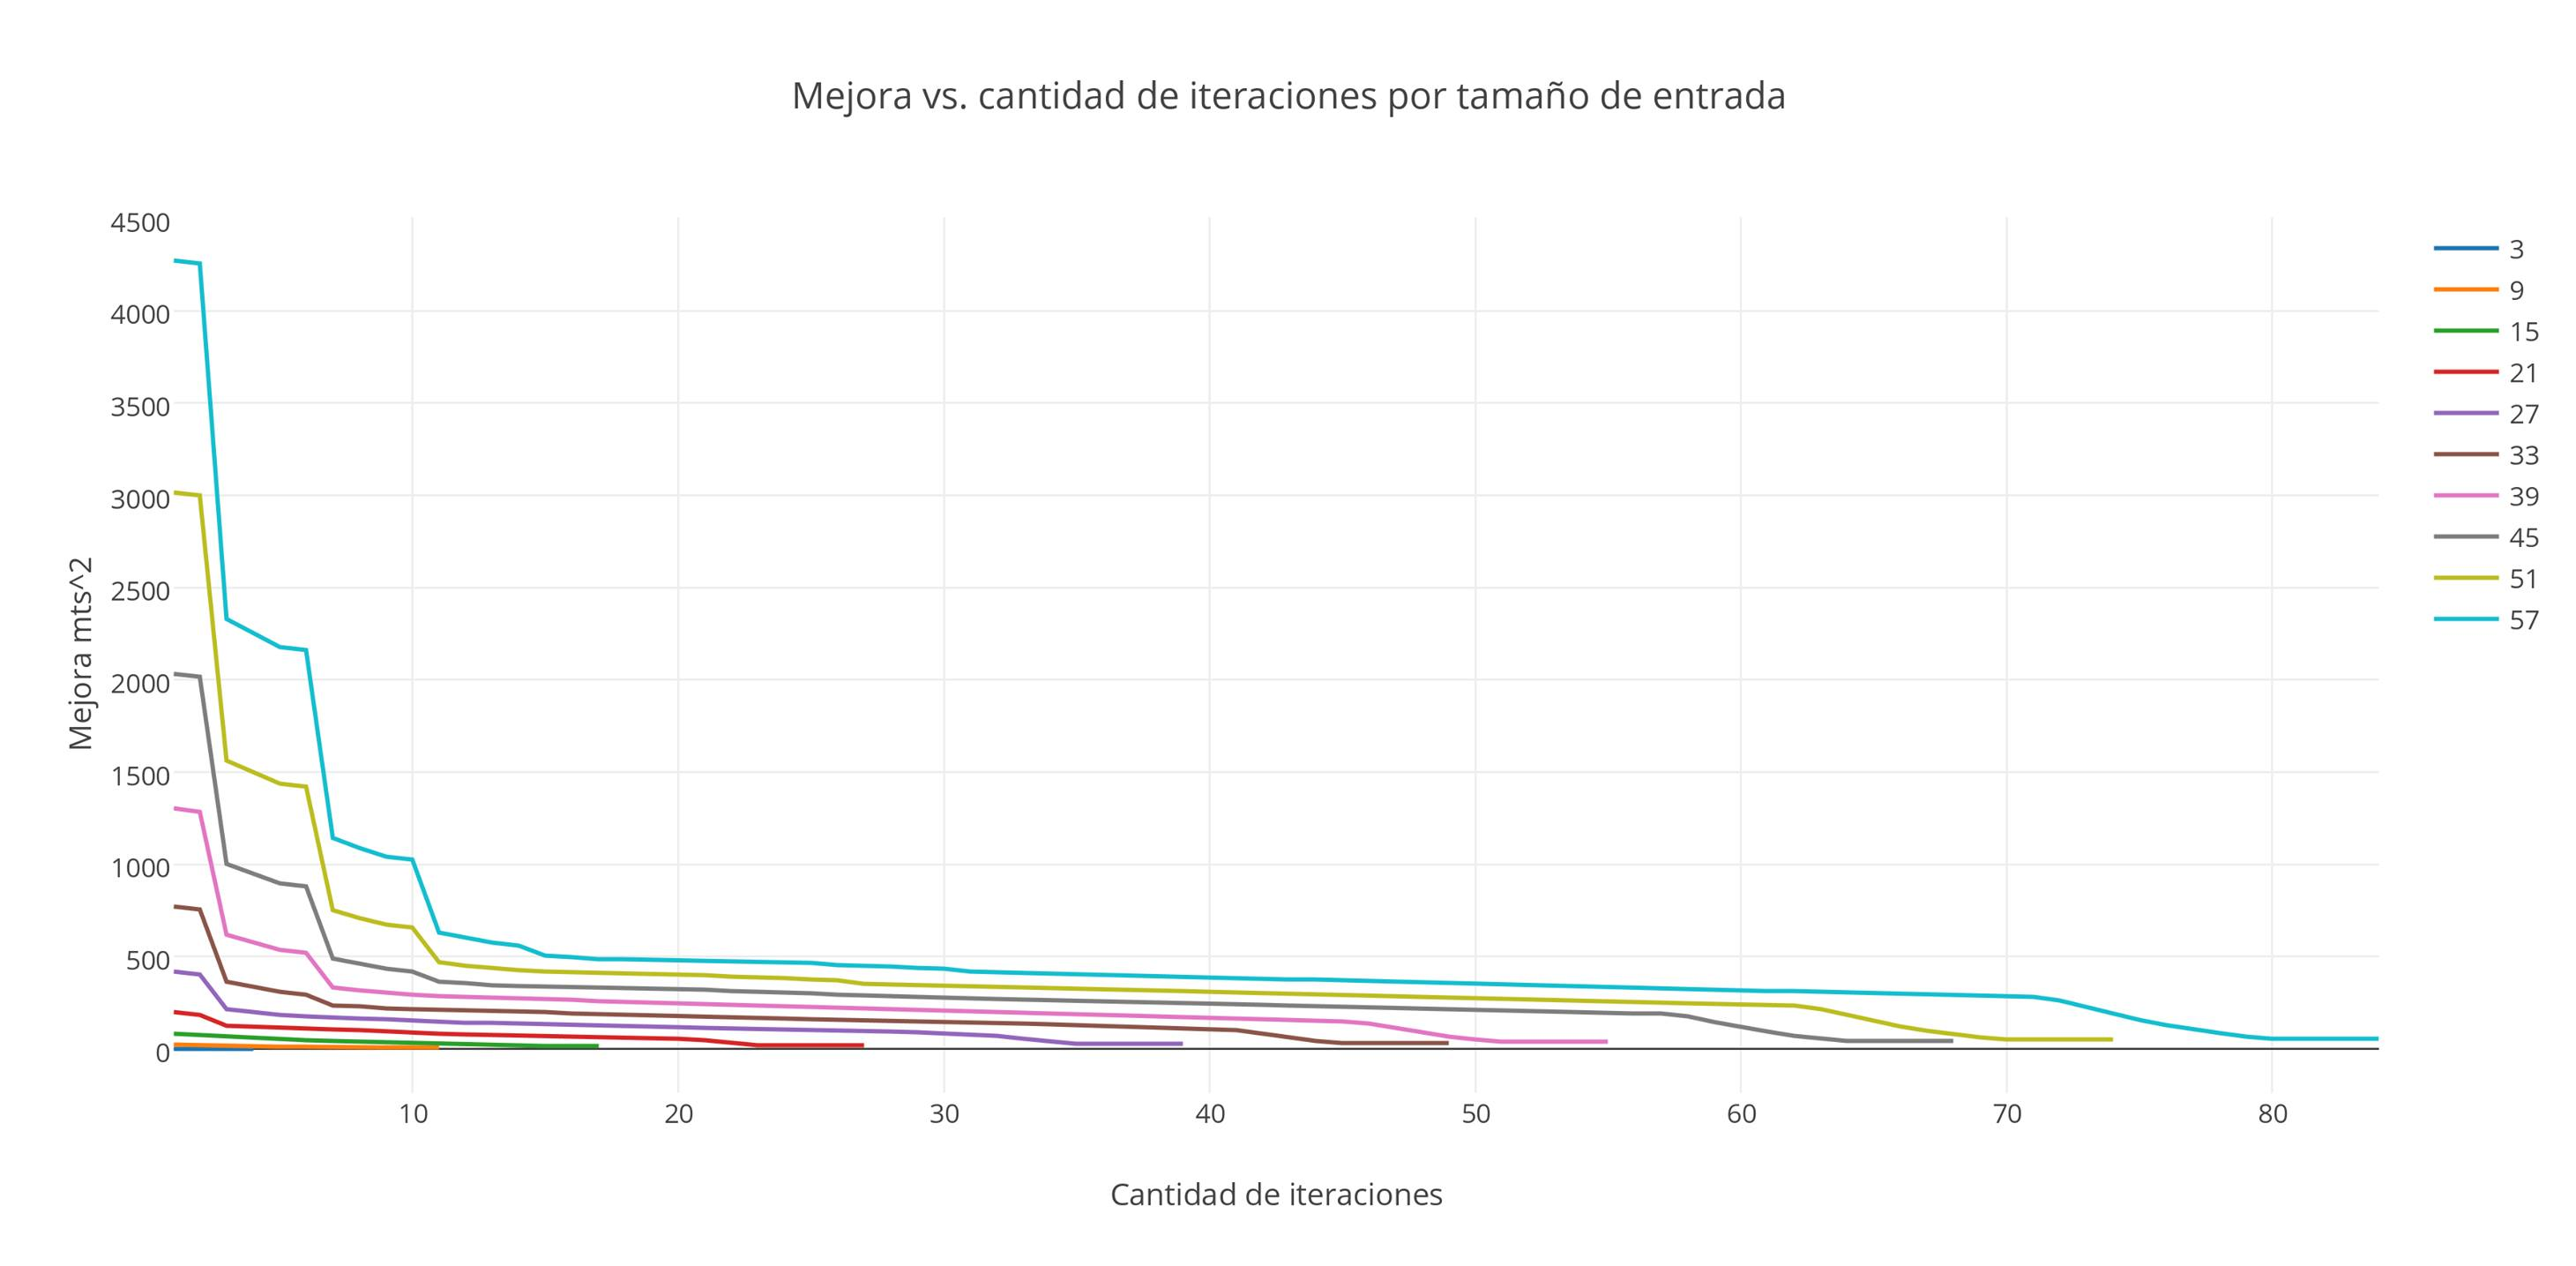
\includegraphics[scale=0.5]{./EJ4/mejora1.png}\\
 {            \textit{Gráfico \ 4.12 - Tabu 2-OPT vs Tabu 3-OPT sobre Familia 6}}
  \end{center}
  \vspace*{0.3cm}
  
  \vspace*{0.3cm} \vspace*{0.3cm}
  \begin{center}
 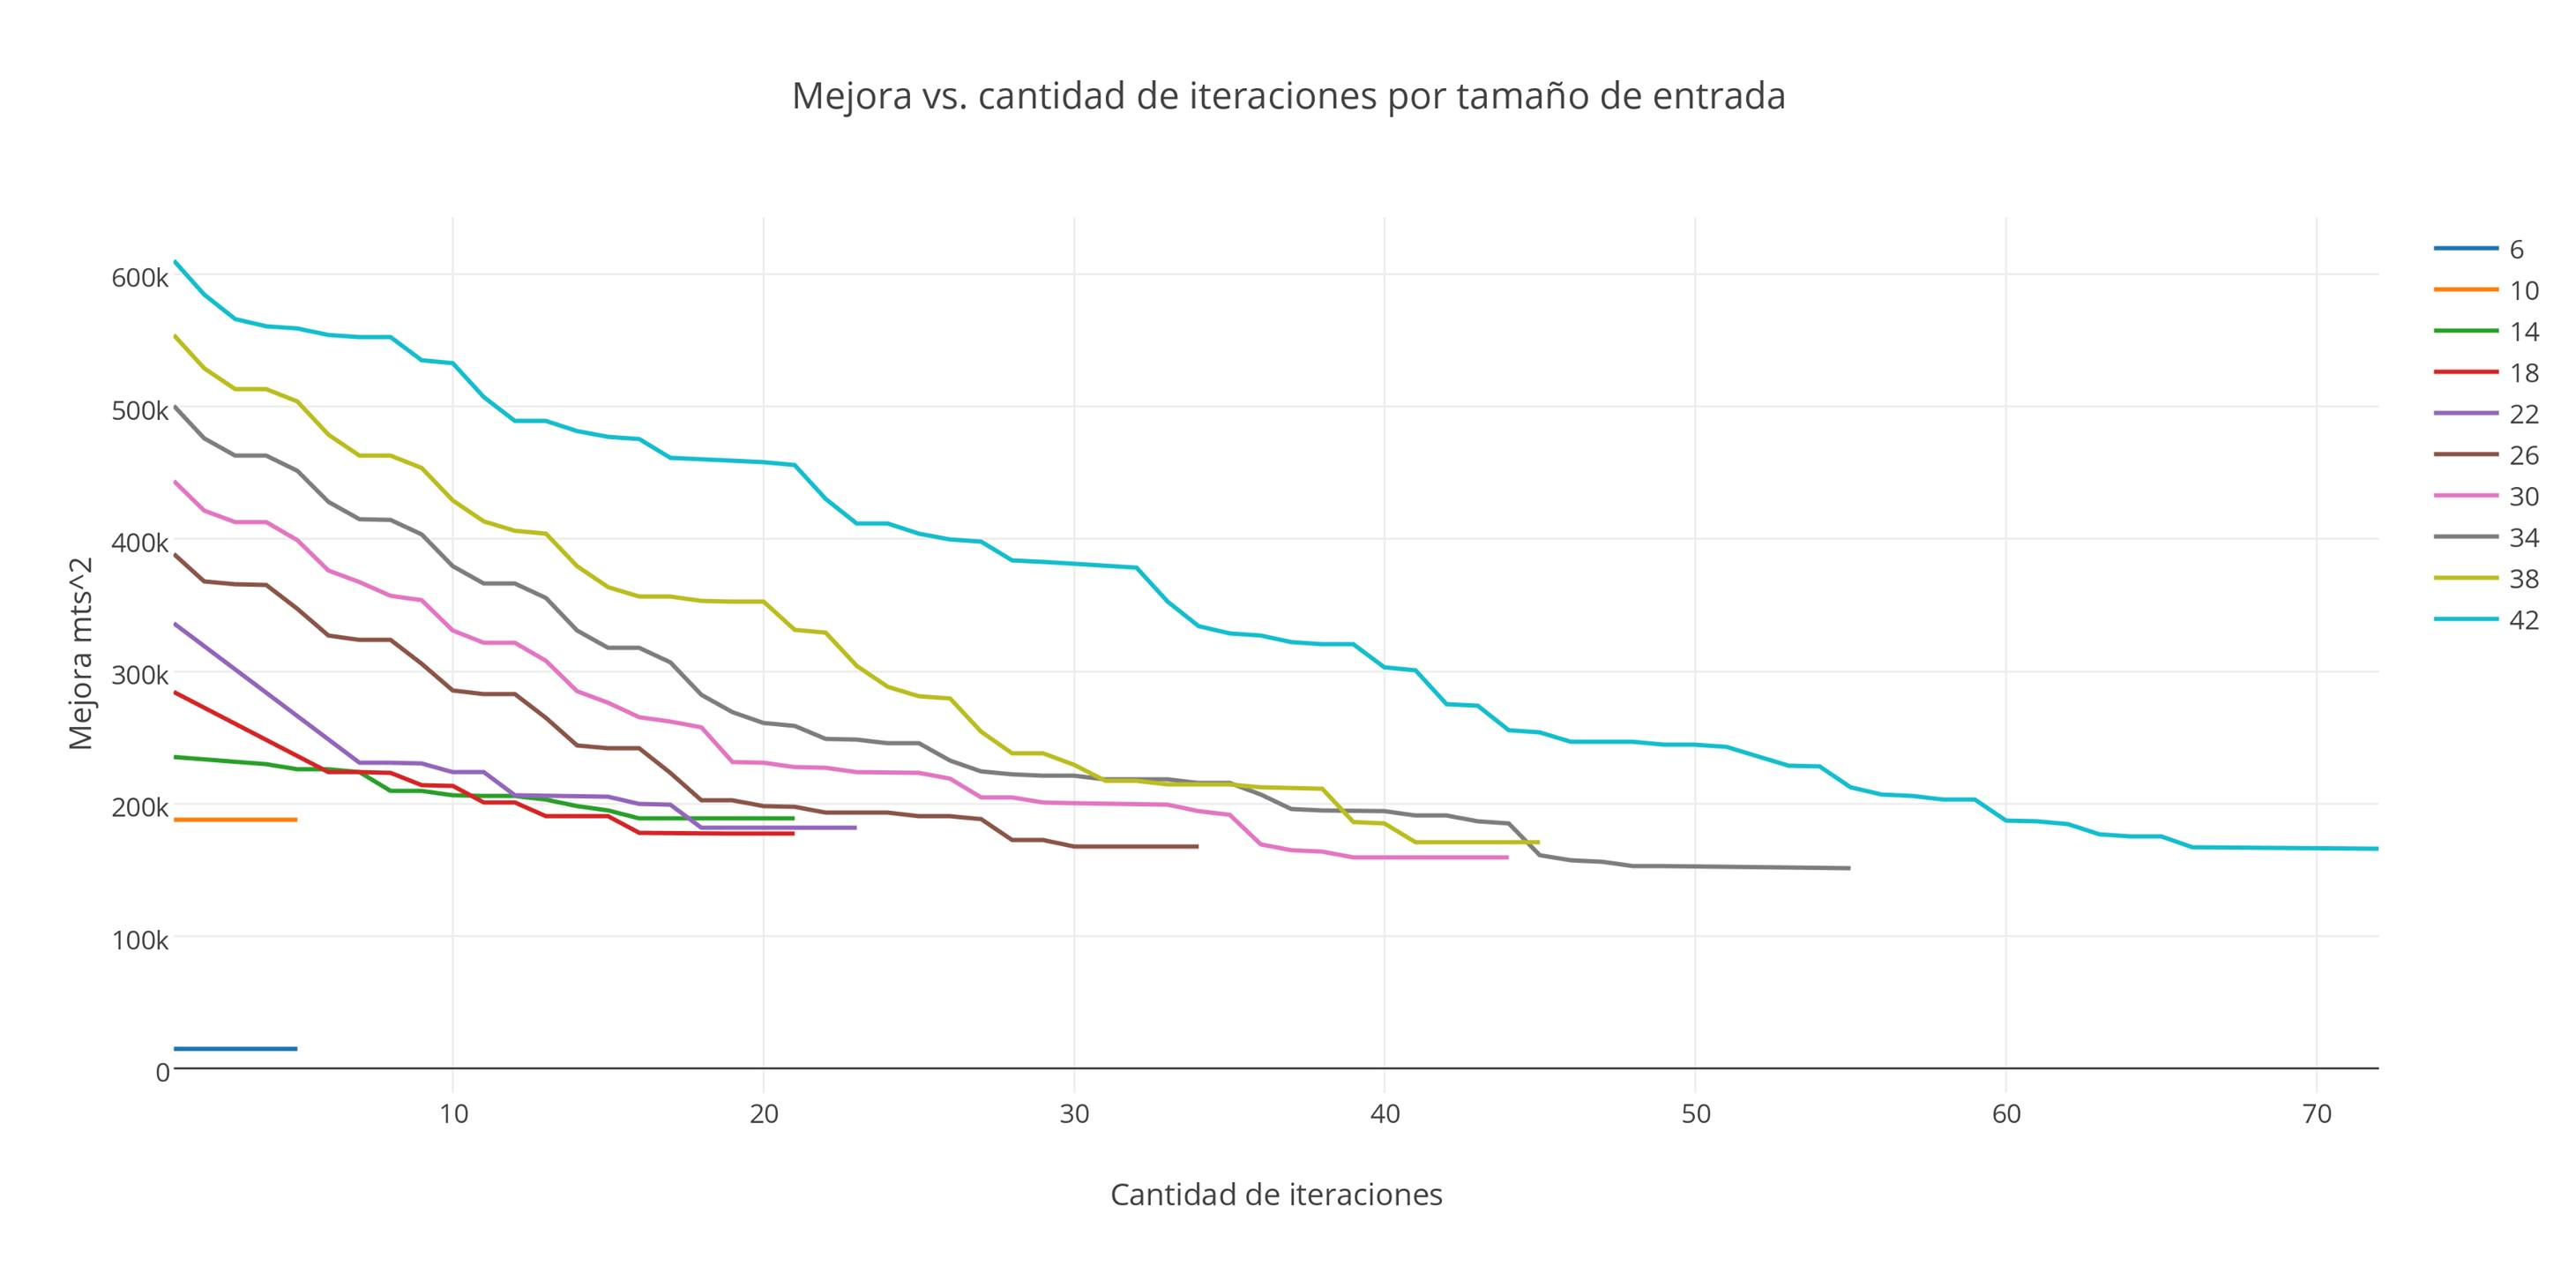
\includegraphics[scale=0.5]{./EJ4/mejora2.png}\\
 {            \textit{Gráfico \ 4.12 - Tabu 2-OPT vs Tabu 3-OPT sobre Familia 6}}
  \end{center}
  \vspace*{0.3cm}
  